\section{Résultats}
\label{sec:resultats}

Cette section présente l'ensemble des résultats empiriques produits par les
scripts R et Python. Toutes les figures sont issues de
\texttt{results/figures/} et tous les tableaux de \texttt{results/tables/}.

\subsection{Analyse exploratoire des données (EDA)}

\subsubsection{Statistiques descriptives}
Le tableau~\ref{tab:desc} résume les trois séries. La charge (\texttt{Load})
est la plus stable (écart-type \(\approx 10\,015\)~MW, quasi-symétrique :
skewness \(\approx 0\)) et présente une kurtosis négative (\(-1{,}10\)),
indice d'une distribution en plateau typique d'un cycle journalier
régulier. \texttt{Wind} et \texttt{Solar} sont fortement asymétriques
(skewness \(1{,}14\) et \(1{,}54\)) et bornées à gauche (\(0\) pour le solaire
la nuit, minimum \(135\)~MW pour l'éolien), ce qui traduit des distributions à
queue droite.

\begin{table}[H]
\centering
\caption{Statistiques descriptives (MW) des trois séries.
Source : \texttt{descriptive\_statistics\_py.csv}.}
\label{tab:desc}
\small
\begin{tabular}{lrrrrrrrrr}
\toprule
Variable & Moyenne & Écart-type & Min & Q1 & Médiane & Q3 & Max & Skew & Kurt. \\
\midrule
\texttt{Load}  & 55\,492 & 10\,015 & 31\,307 & 47\,106 & 55\,092 & 64\,309 & 77\,549 & $-0{,}01$ & $-1{,}10$ \\
\texttt{Wind}  & 11\,552 & 9\,076 & 135 & 4\,506 & 9\,015 & 16\,114 & 46\,064 & 1{,}14 & 0{,}76 \\
\texttt{Solar} & 4\,566 & 6\,940 & 0 & 0 & 173 & 7\,342 & 32\,947 & 1{,}54 & 1{,}38 \\
\bottomrule
\end{tabular}
\end{table}

\subsubsection{Évolution temporelle et vue d'ensemble}
La figure~\ref{fig:ts_overview} donne une vue d'ensemble des trois séries sur
les \(50\,400\) heures, complétée par les figures~\ref{fig:load_ts},
\ref{fig:wind_ts} et~\ref{fig:solar_ts}. On y lit une saisonnalité annuelle
nette (creux de charge en août, pic hivernal), un profil solaire
parfaitement nul la nuit, et un éolien très volatil sans cycle annuel marqué.

\begin{figure}[H]
\centering
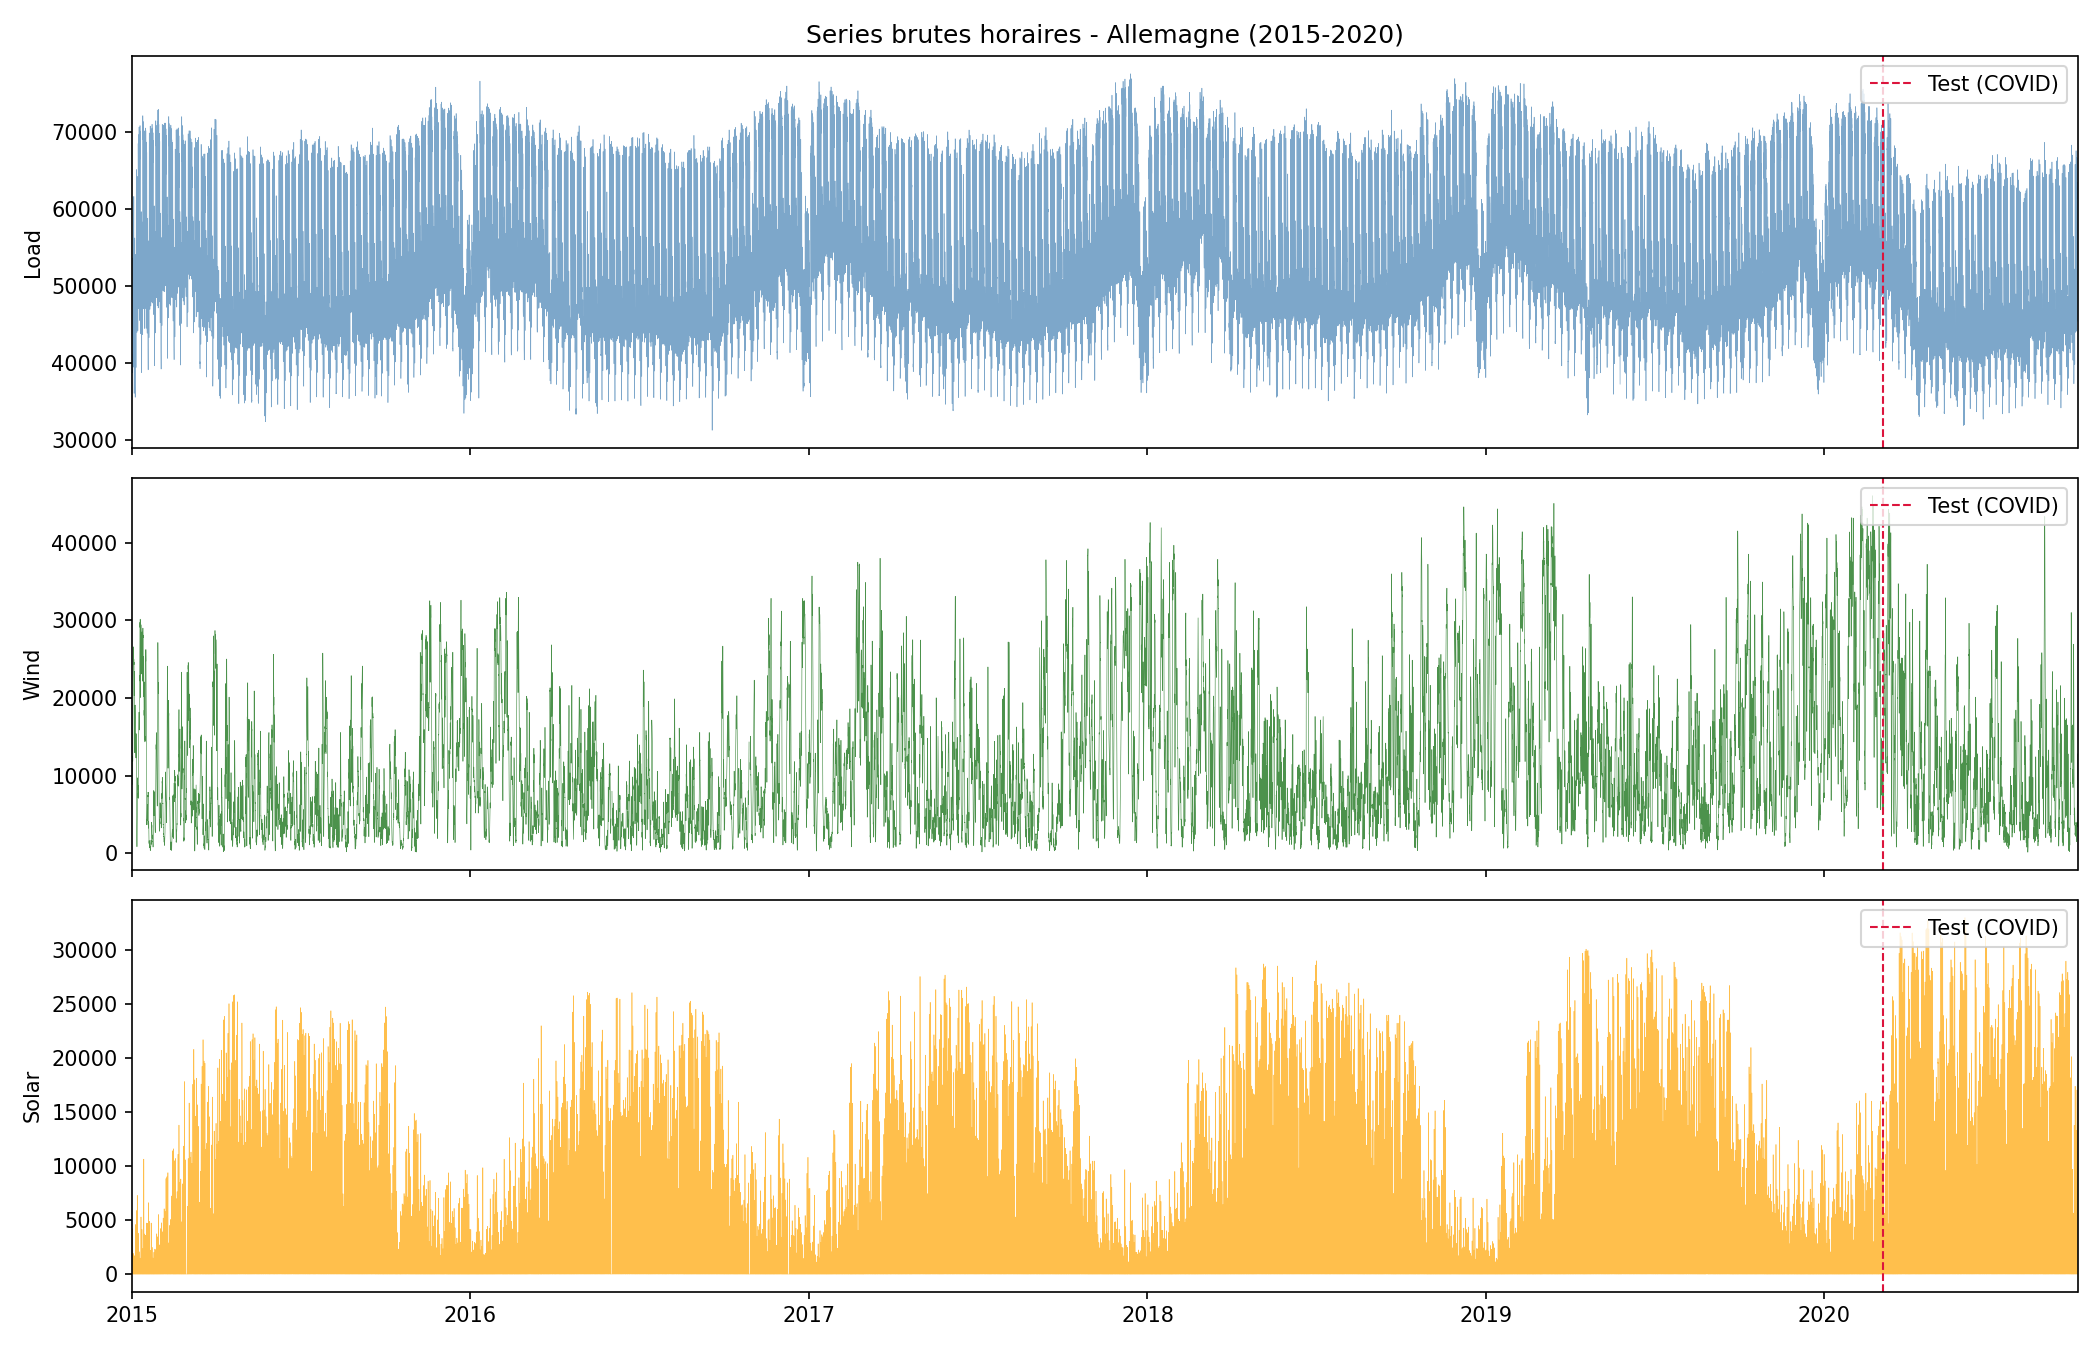
\includegraphics[width=0.95\textwidth]{py_ts_overview.png}
\caption{Vue d'ensemble des trois séries horaires (2015--2020).}
\label{fig:ts_overview}
\end{figure}

\begin{figure}[H]
\centering
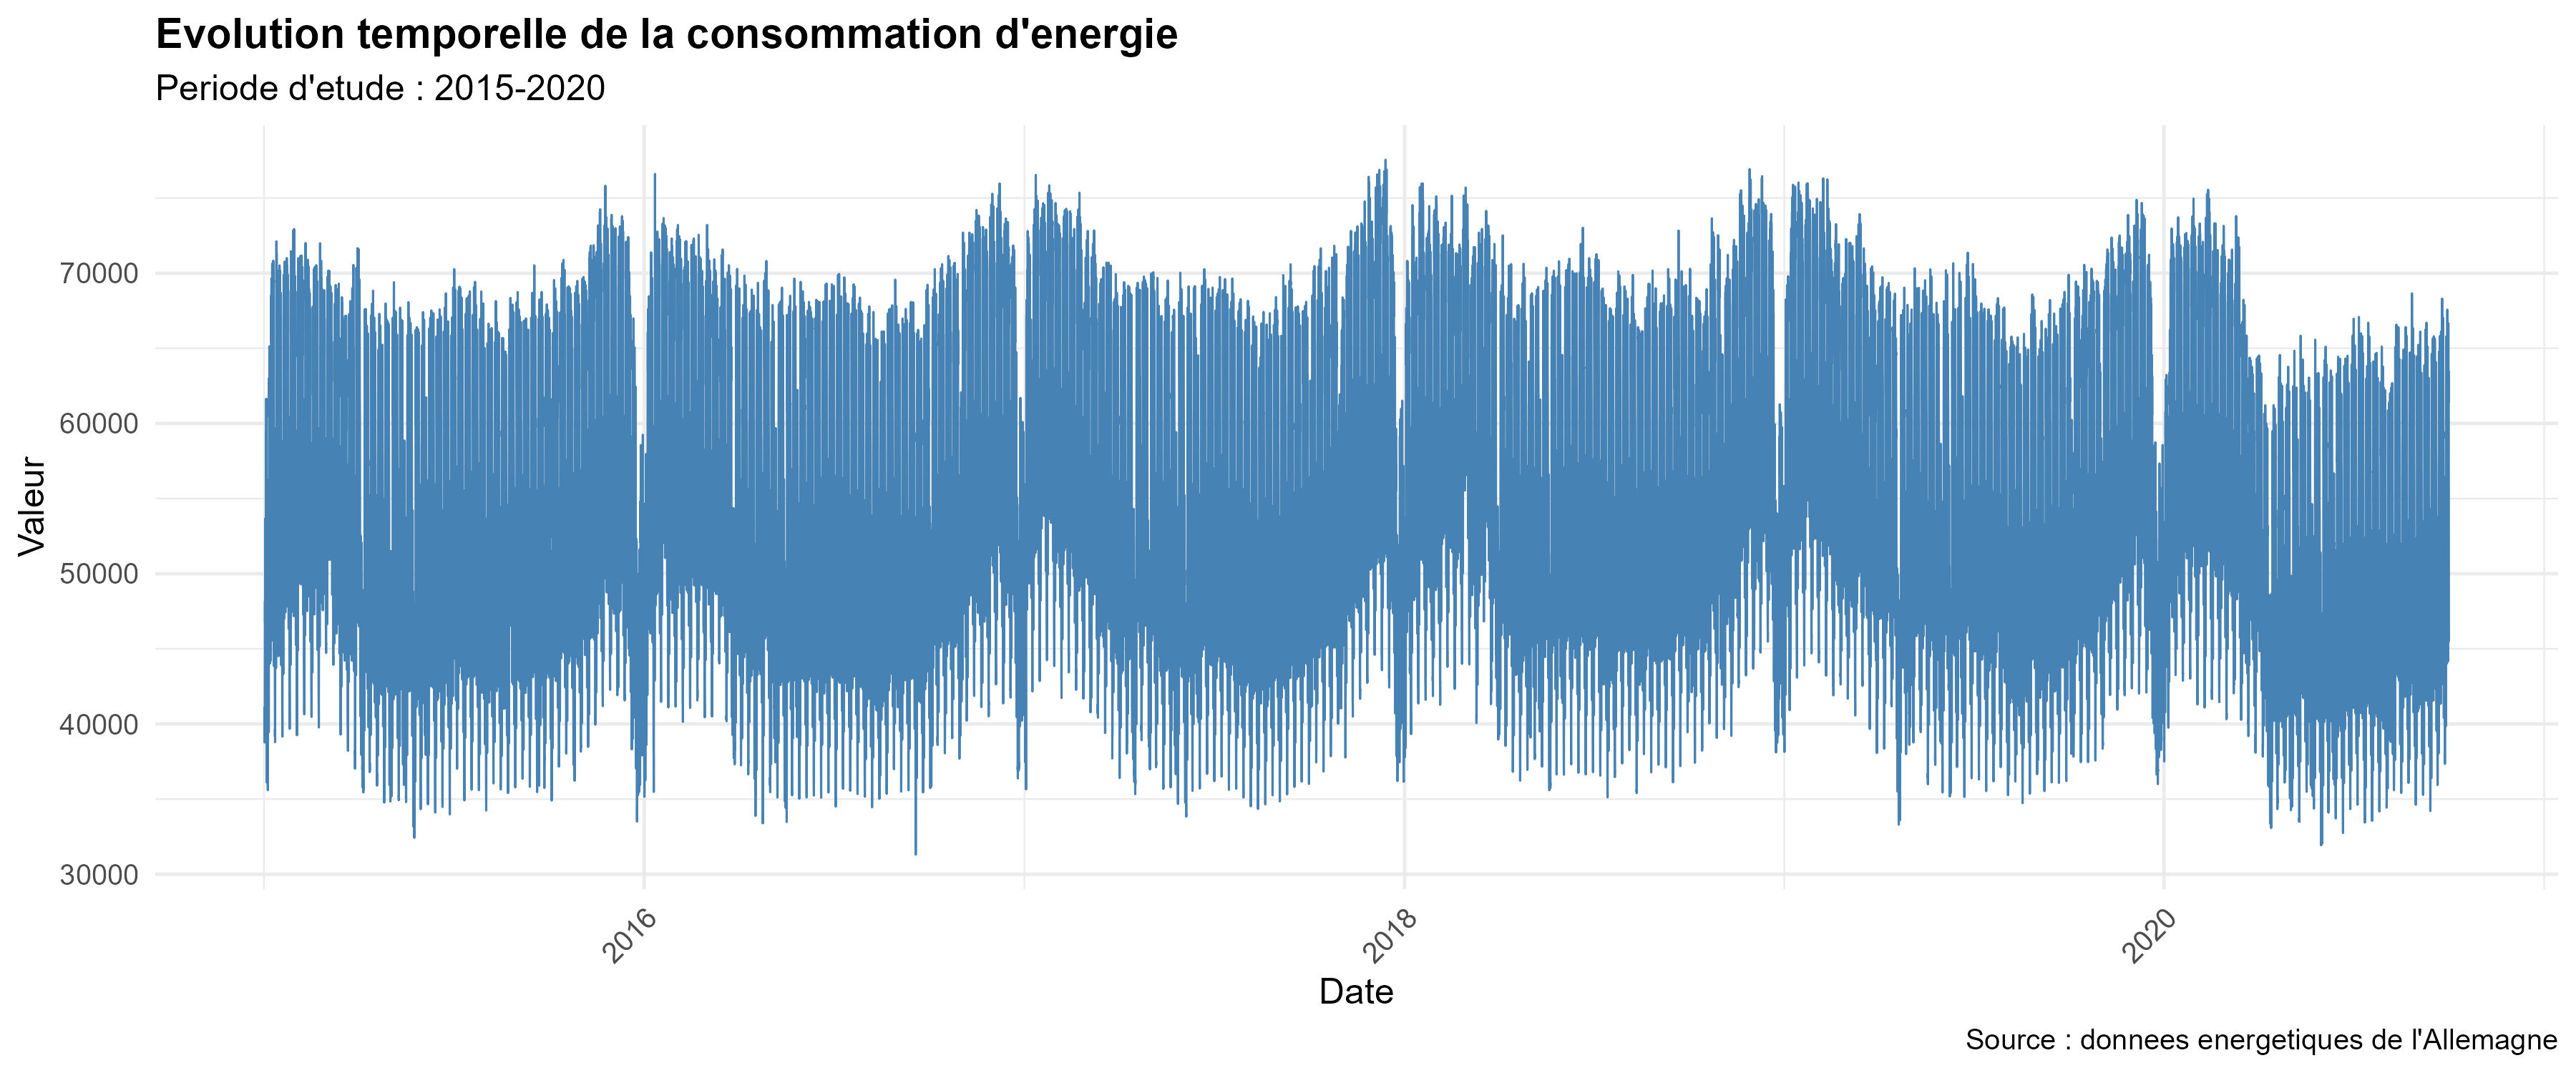
\includegraphics[width=0.9\textwidth]{Load_time_series.png}
\caption{Évolution temporelle de la consommation (\texttt{Load}).}
\label{fig:load_ts}
\end{figure}

\begin{figure}[H]
\centering
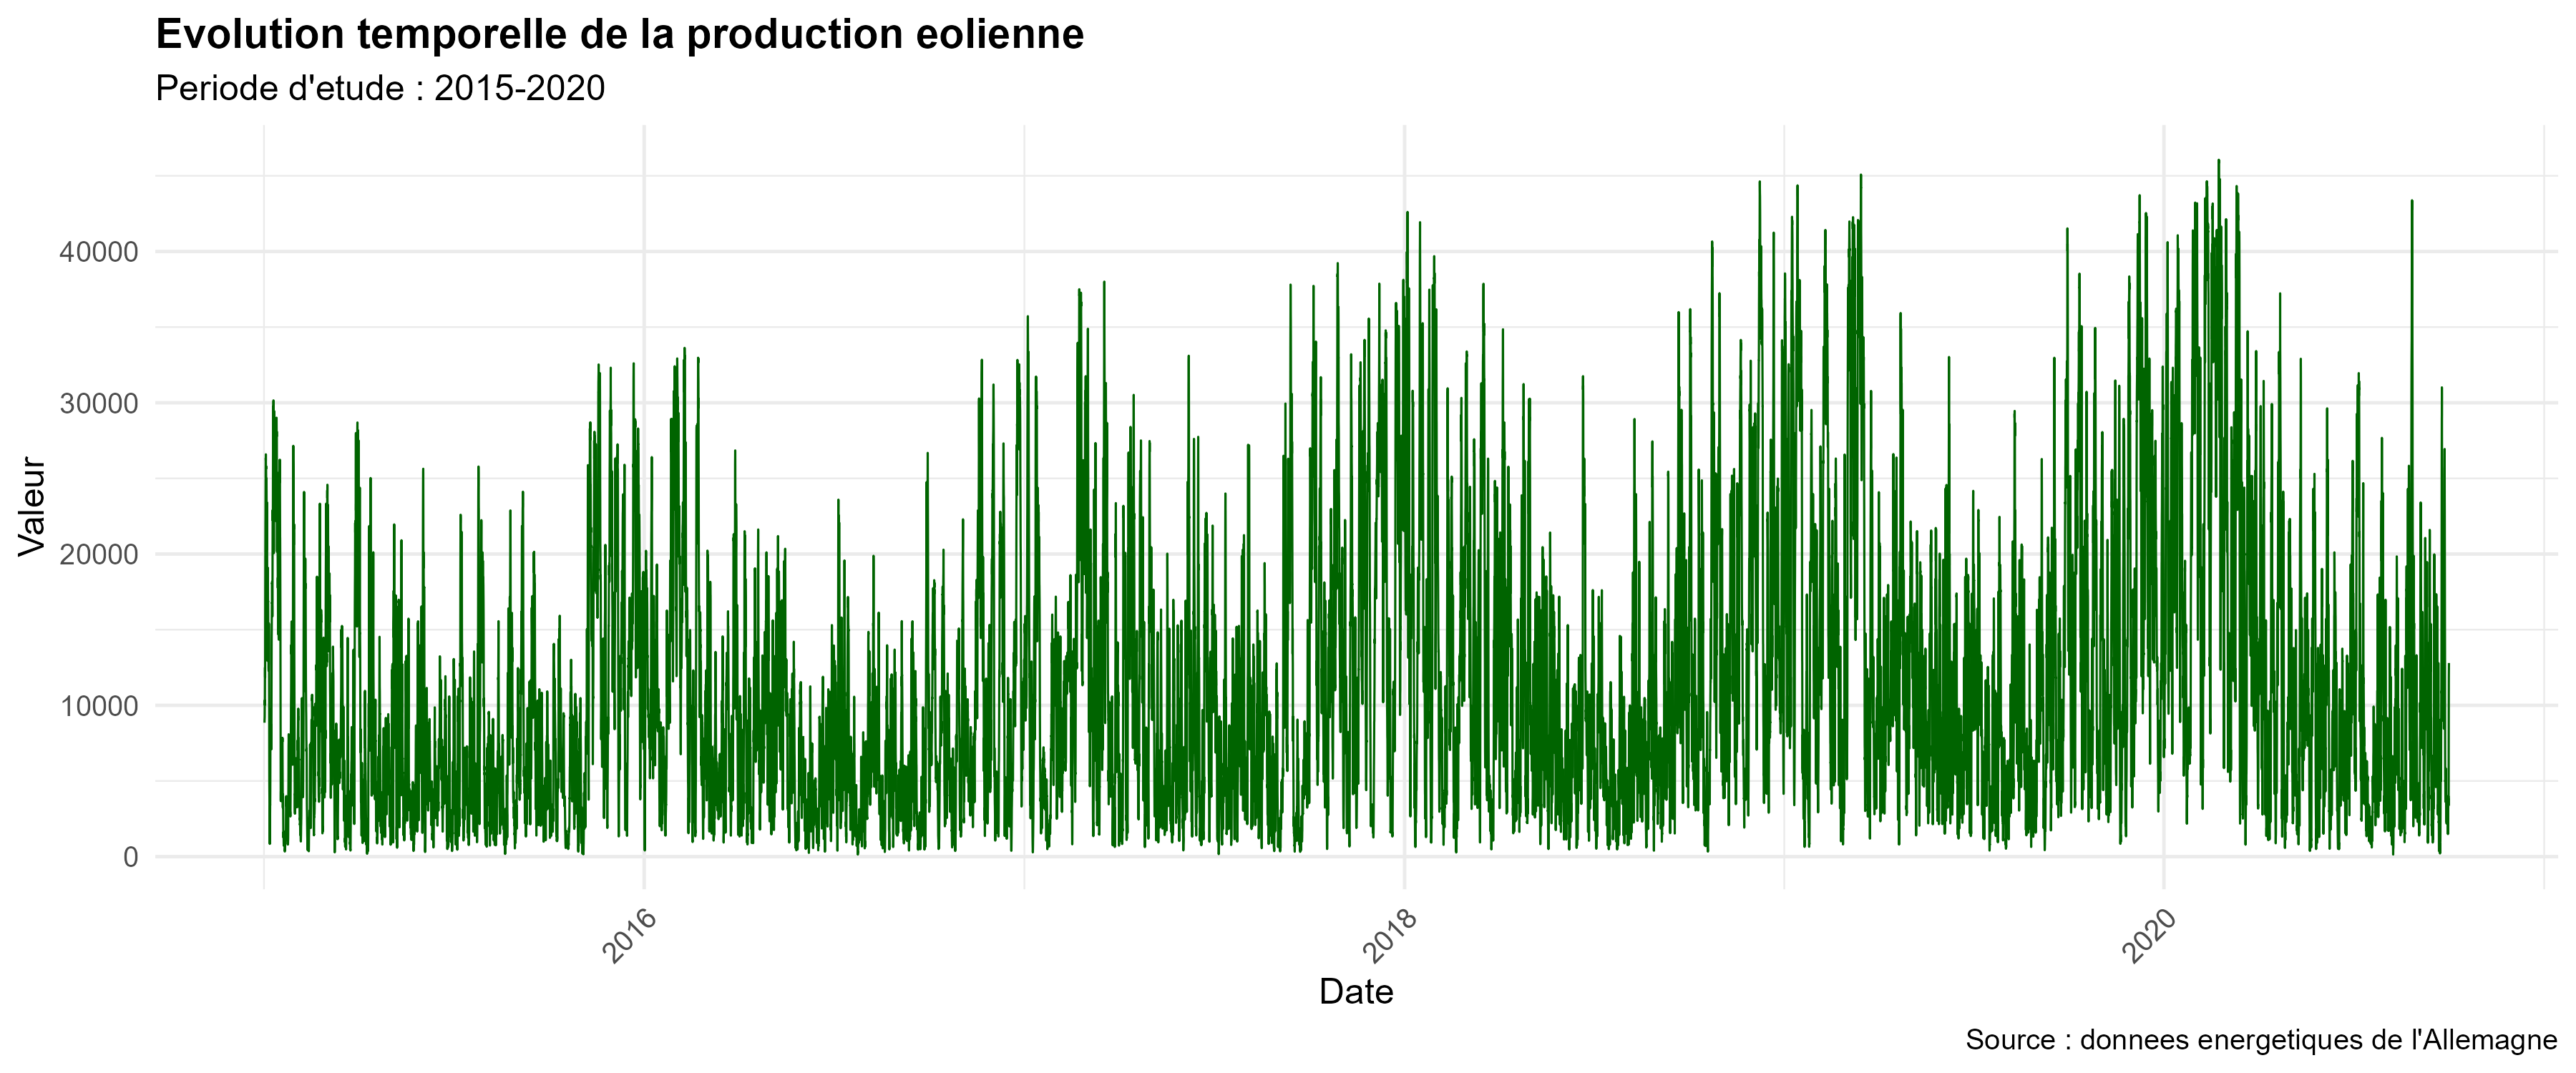
\includegraphics[width=0.9\textwidth]{Wind_time_series.png}
\caption{Évolution temporelle de la production éolienne (\texttt{Wind}).}
\label{fig:wind_ts}
\end{figure}

\begin{figure}[H]
\centering
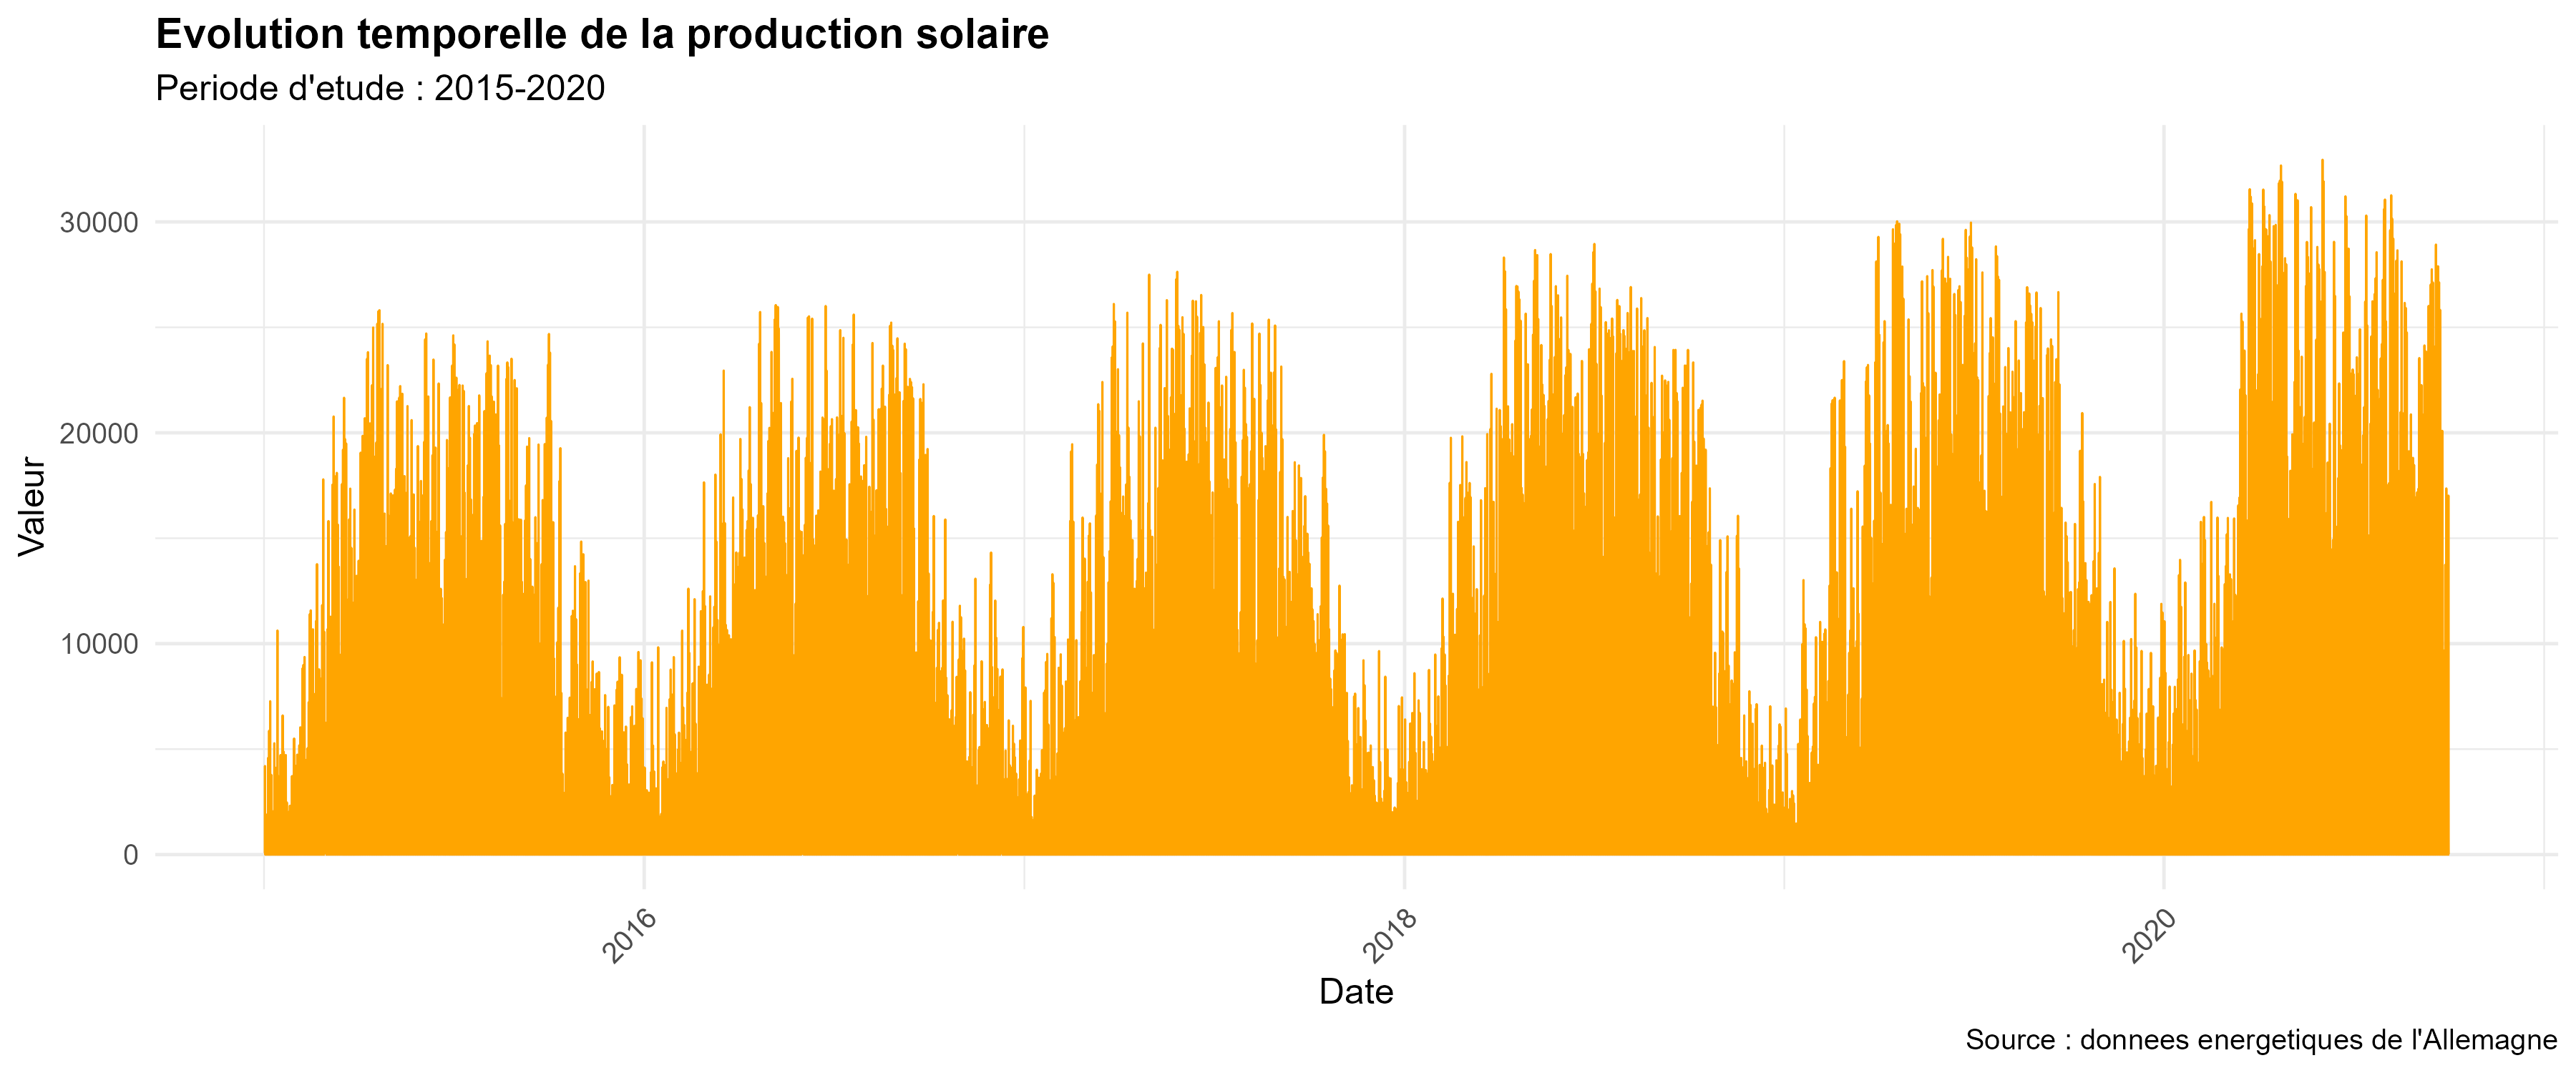
\includegraphics[width=0.9\textwidth]{Solar_time_series.png}
\caption{Évolution temporelle de la production solaire (\texttt{Solar}).}
\label{fig:solar_ts}
\end{figure}

\subsubsection{Profils saisonniers}
Le profil horaire (figure~\ref{fig:hourly}) montre un double pic de charge
(\(\approx 9\)~h et \(19\)~h) et un solaire en cloche centré sur
\(11\)--\(12\)~h. Le profil hebdomadaire (figure~\ref{fig:weekly}) révèle une
baisse de la charge le week-end, alors que la production renouvelable est
indépendante du jour de la semaine. Le profil mensuel (figure~\ref{fig:monthly})
oppose un éolien hivernal (max en décembre) à un solaire estival (max en
juin--juillet). L'évolution annuelle (figure~\ref{fig:yearly}) permet enfin de
suivre ces tendances de fond.

\begin{figure}[H]
\centering
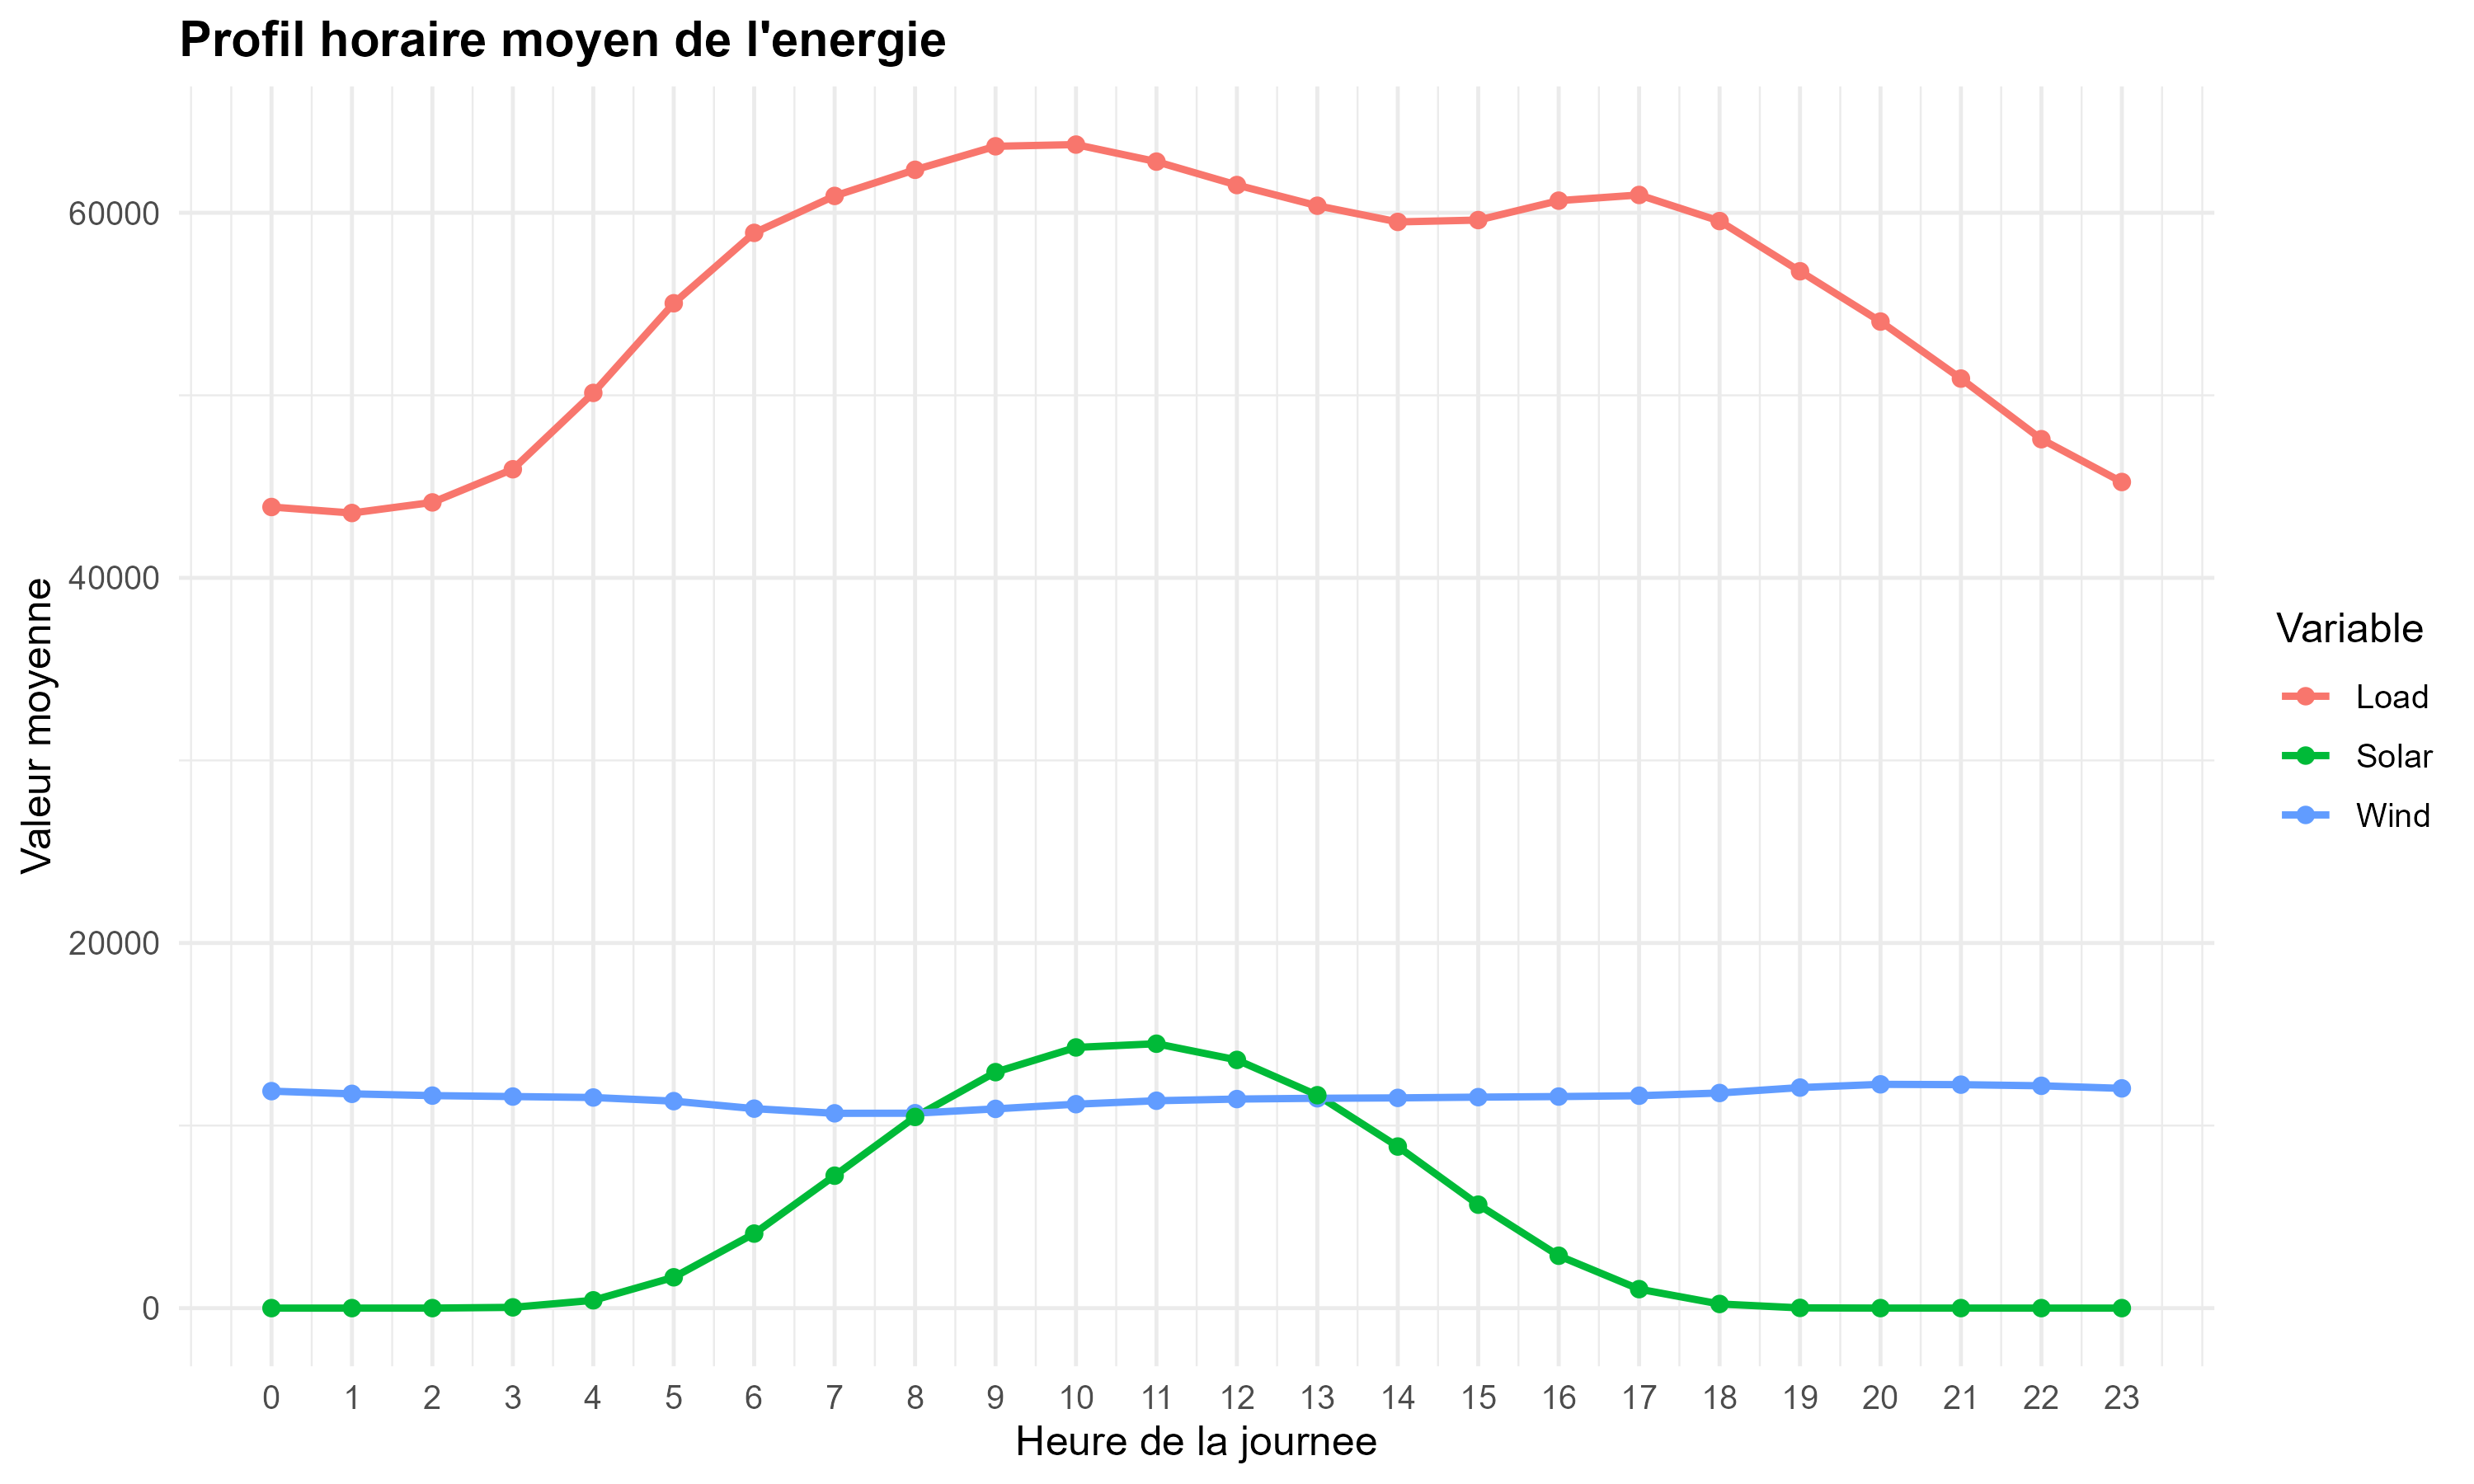
\includegraphics[width=0.85\textwidth]{hourly_profiles.png}
\caption{Profil horaire moyen des trois séries.}
\label{fig:hourly}
\end{figure}

\begin{figure}[H]
\centering
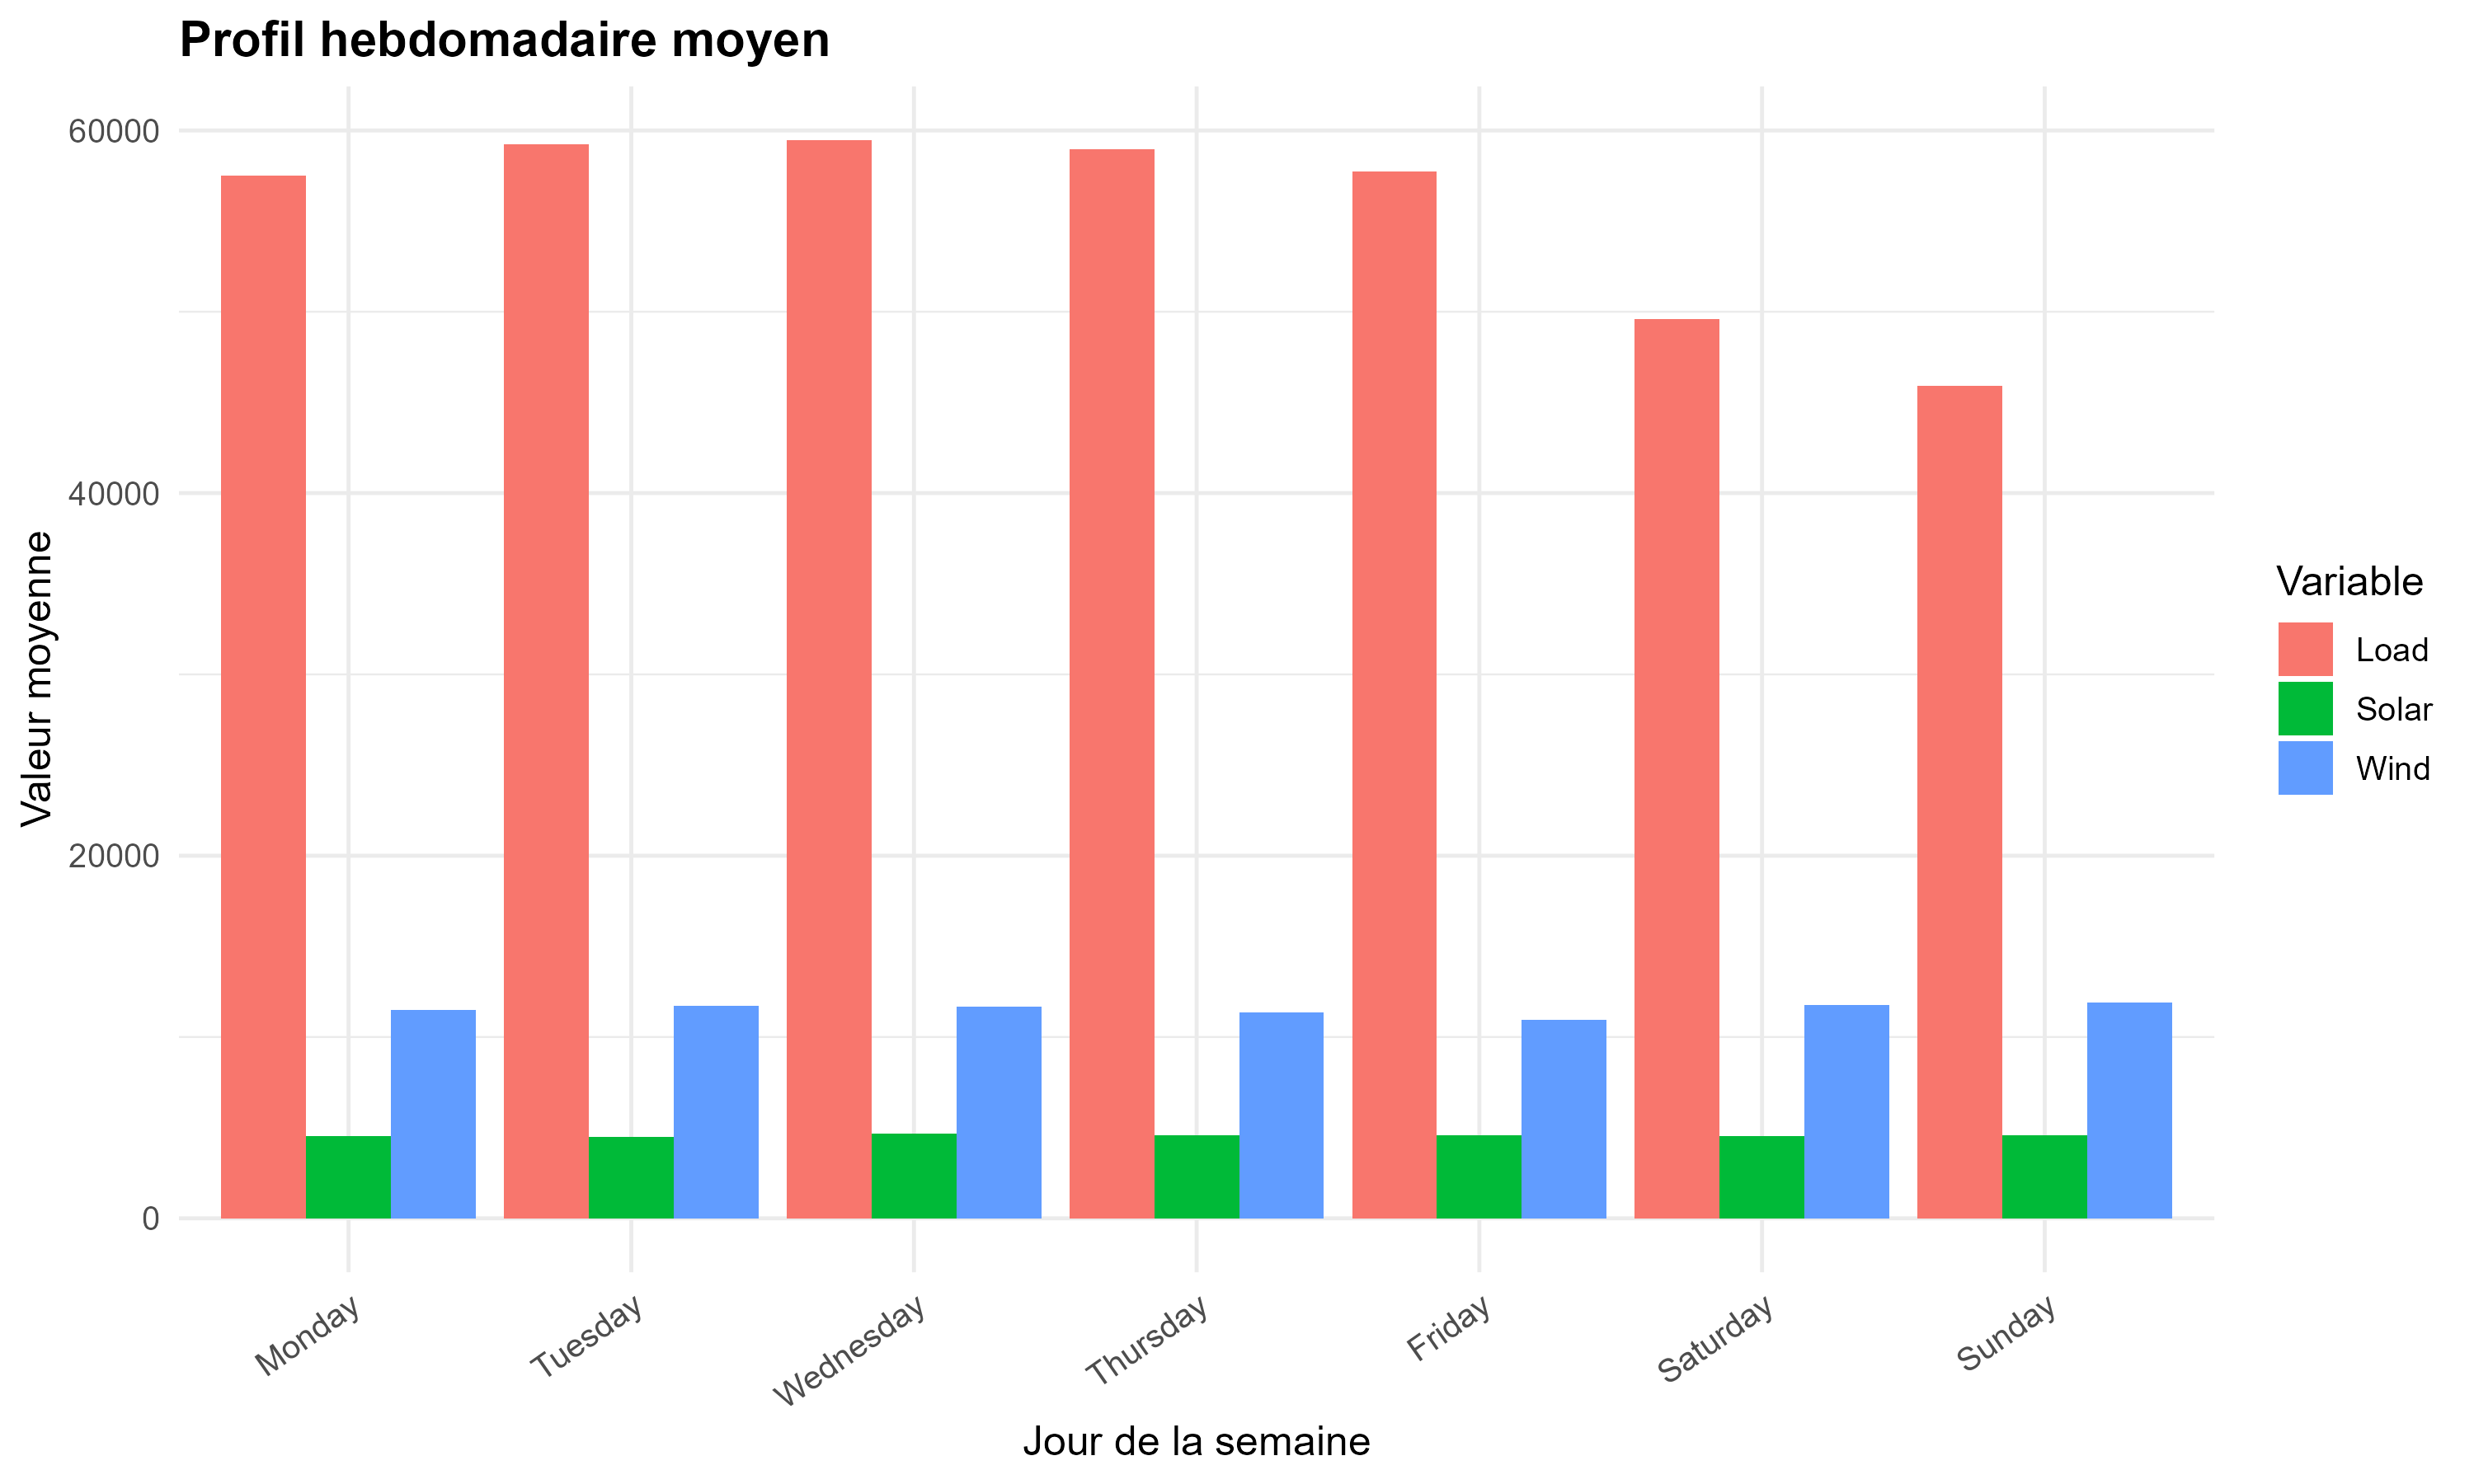
\includegraphics[width=0.85\textwidth]{weekly_profiles.png}
\caption{Profil hebdomadaire moyen.}
\label{fig:weekly}
\end{figure}

\begin{figure}[H]
\centering
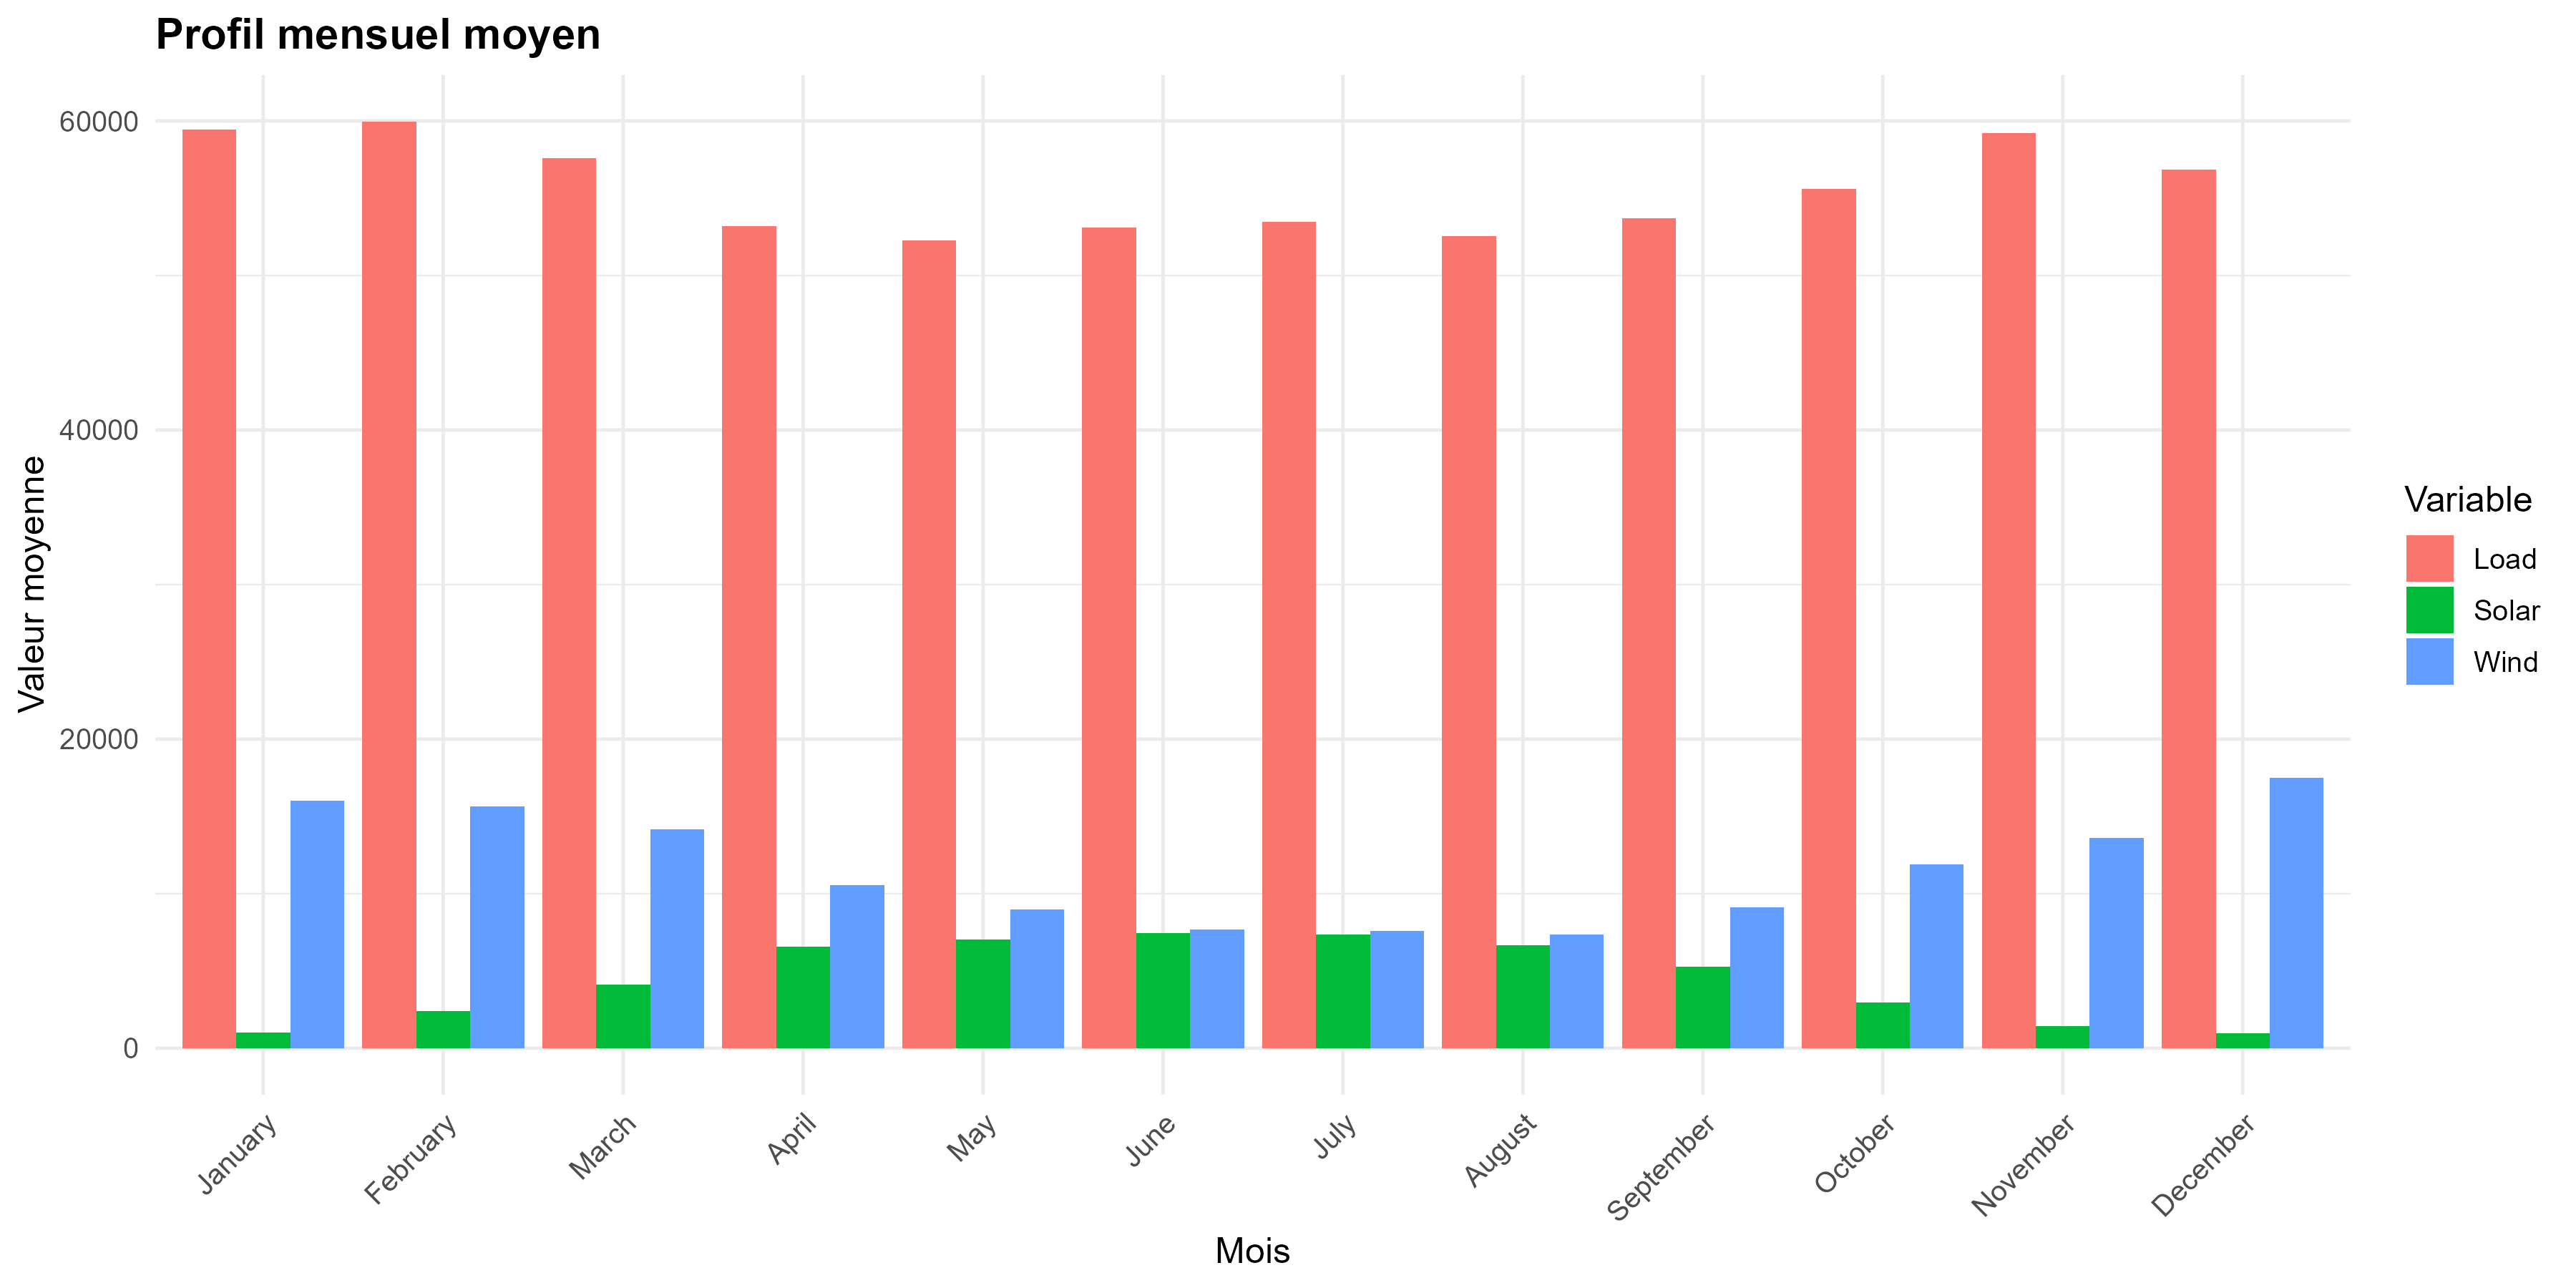
\includegraphics[width=0.9\textwidth]{monthly_profiles.png}
\caption{Profil mensuel moyen.}
\label{fig:monthly}
\end{figure}

\begin{figure}[H]
\centering
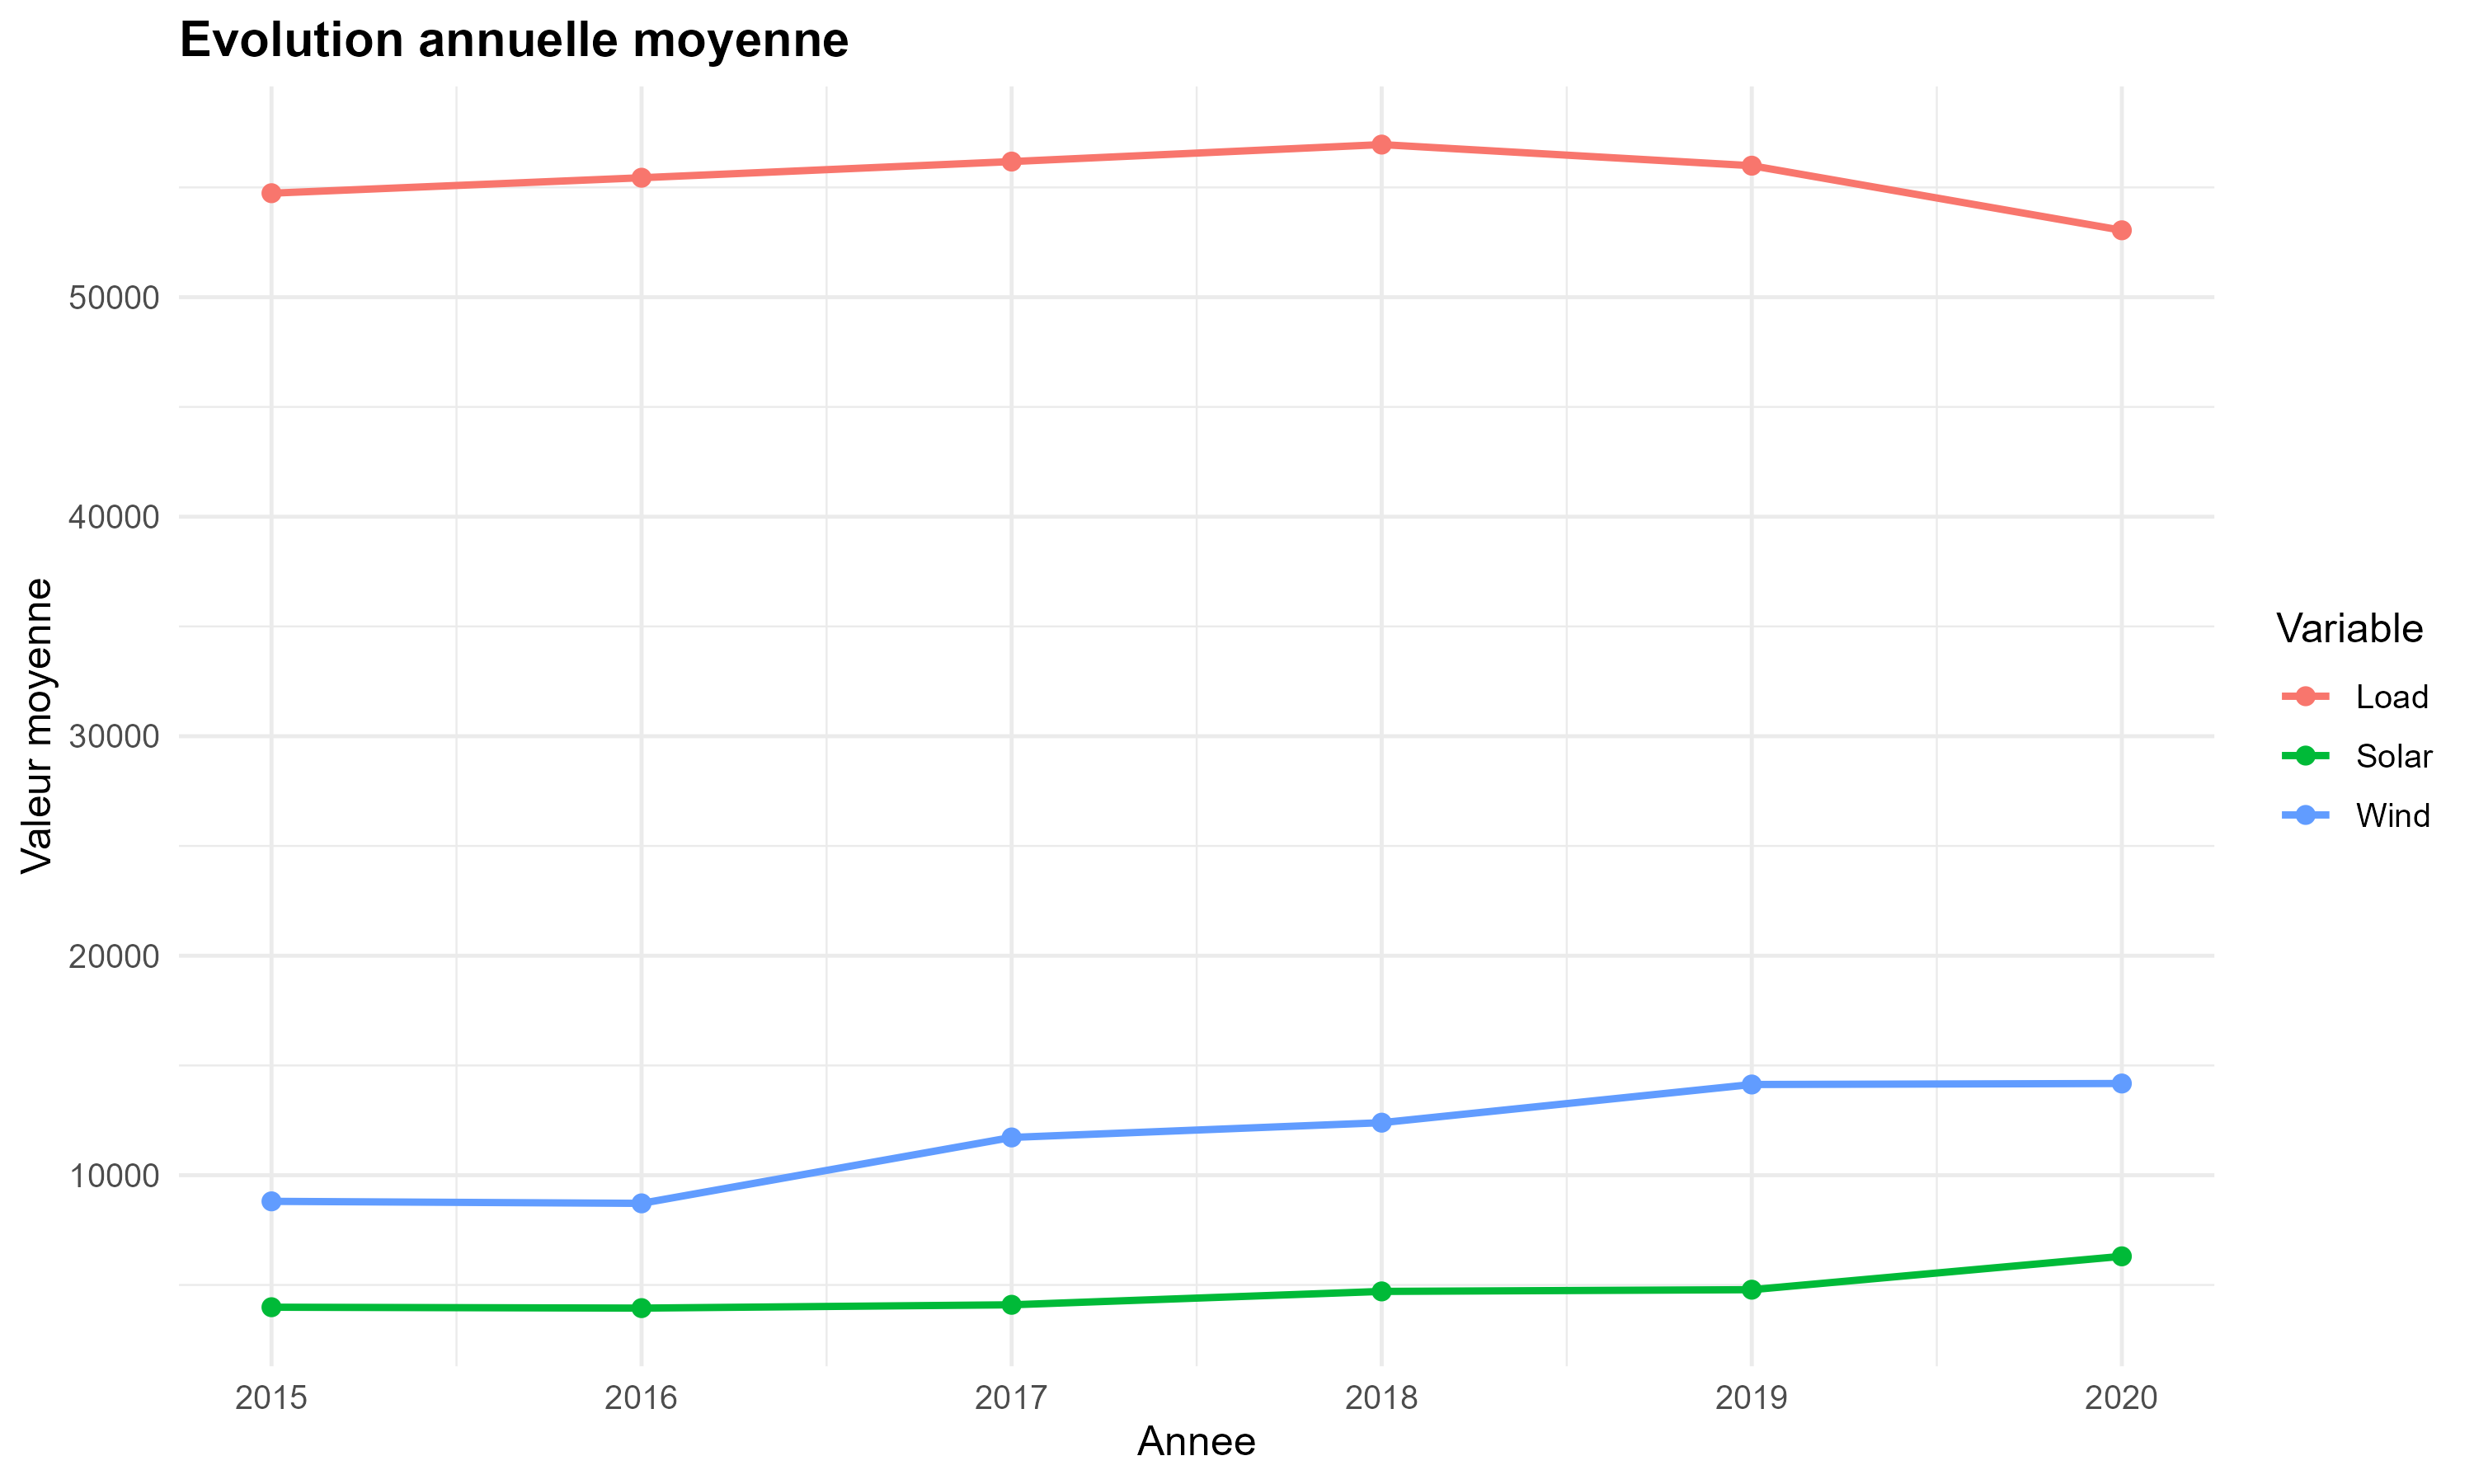
\includegraphics[width=0.8\textwidth]{yearly_profiles.png}
\caption{Évolution annuelle moyenne.}
\label{fig:yearly}
\end{figure}

\begin{figure}[H]
\centering
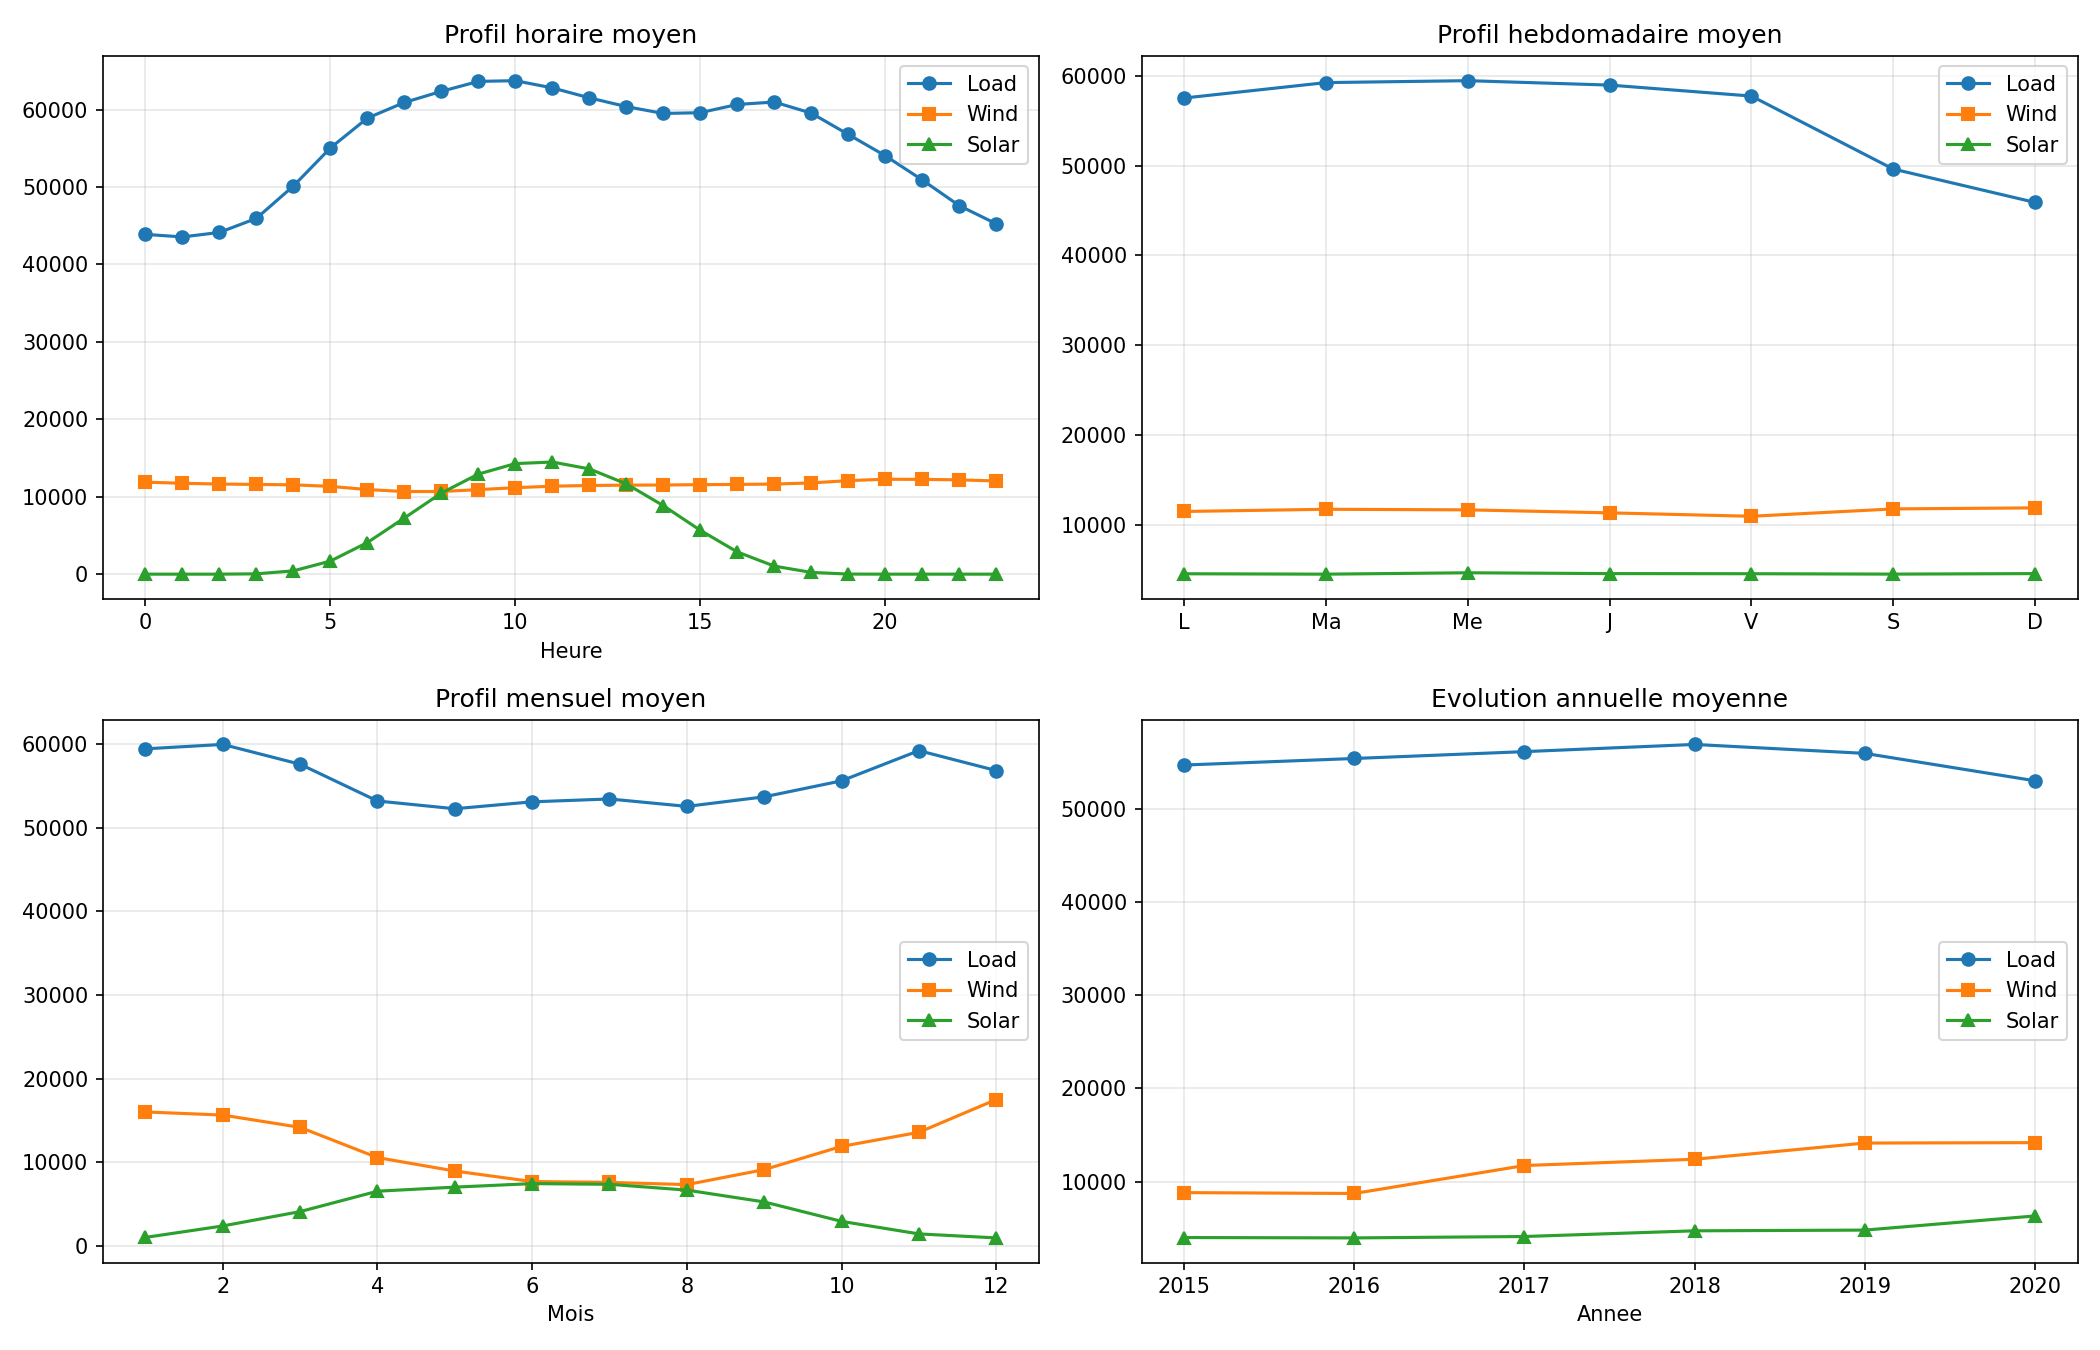
\includegraphics[width=0.9\textwidth]{py_seasonal_profiles.png}
\caption{Profils saisonniers (calcul Python).}
\label{fig:seasonal}
\end{figure}

\begin{figure}[H]
\centering
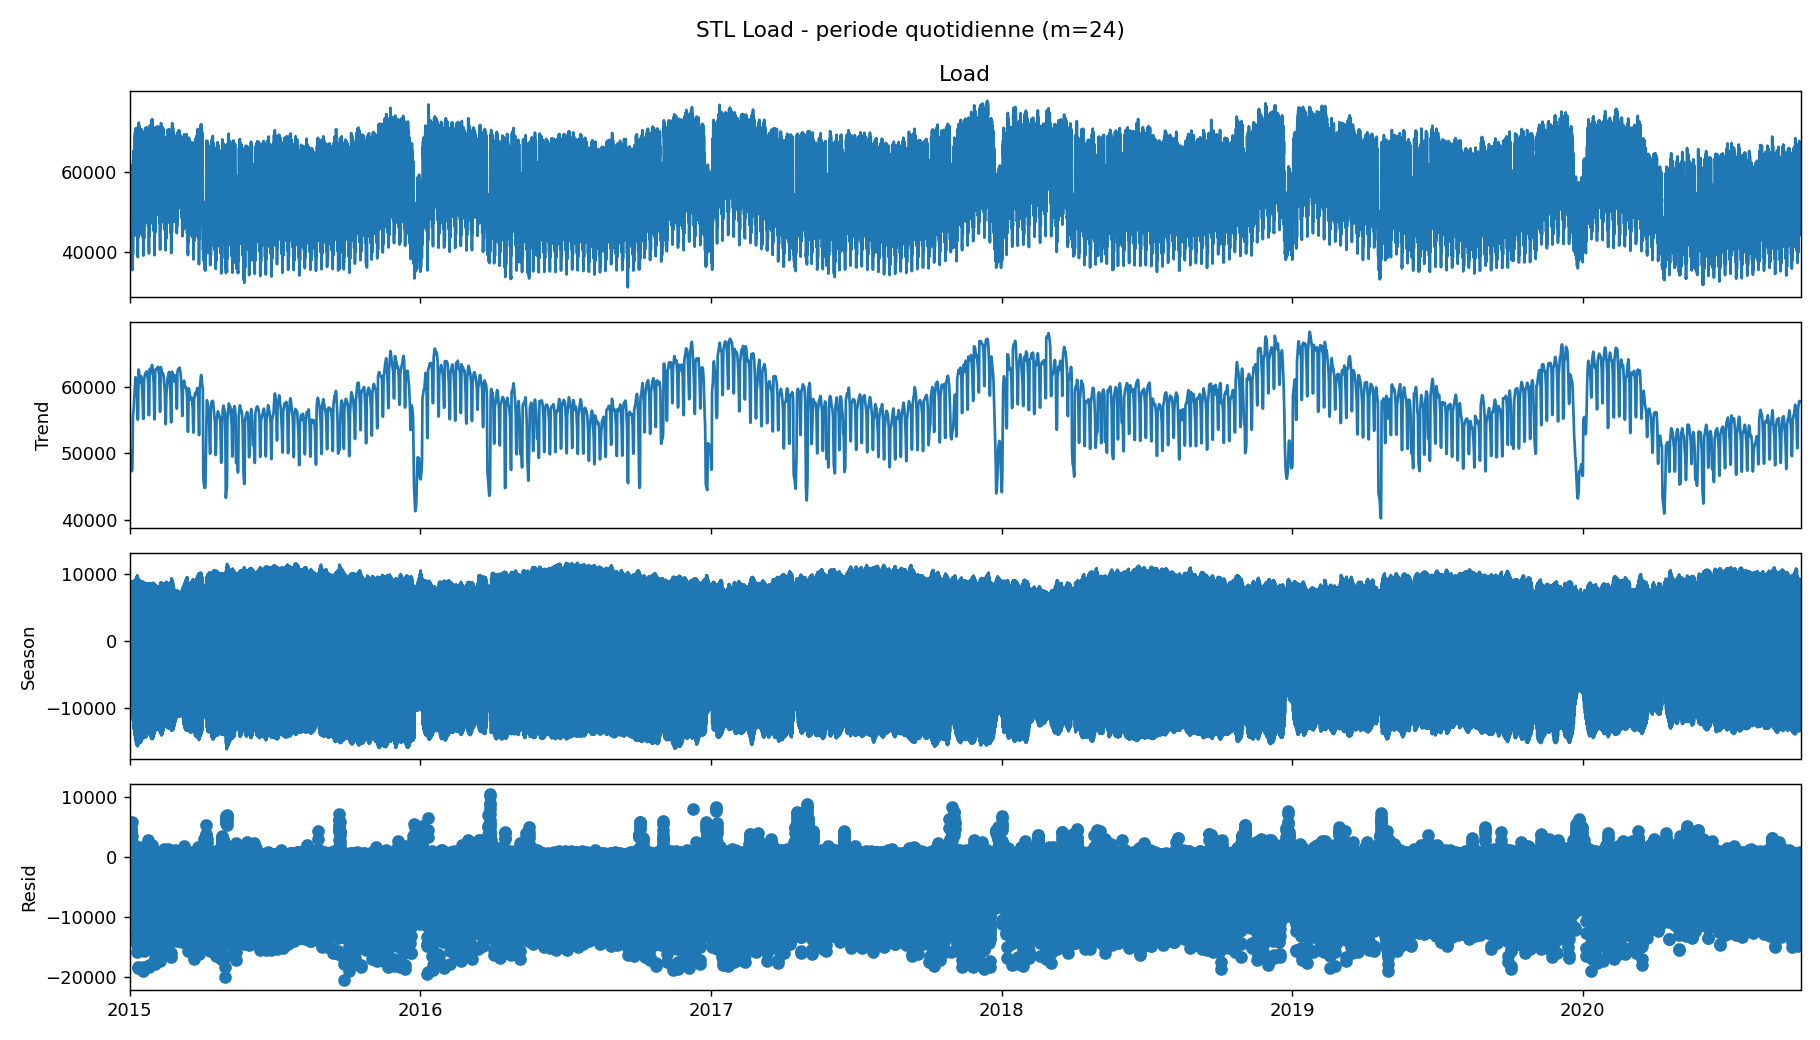
\includegraphics[width=0.75\textwidth]{py_stl_load_daily.png}
\caption{Décomposition STL de la charge (cycle journalier).}
\label{fig:stl_daily}
\end{figure}

\begin{figure}[H]
\centering
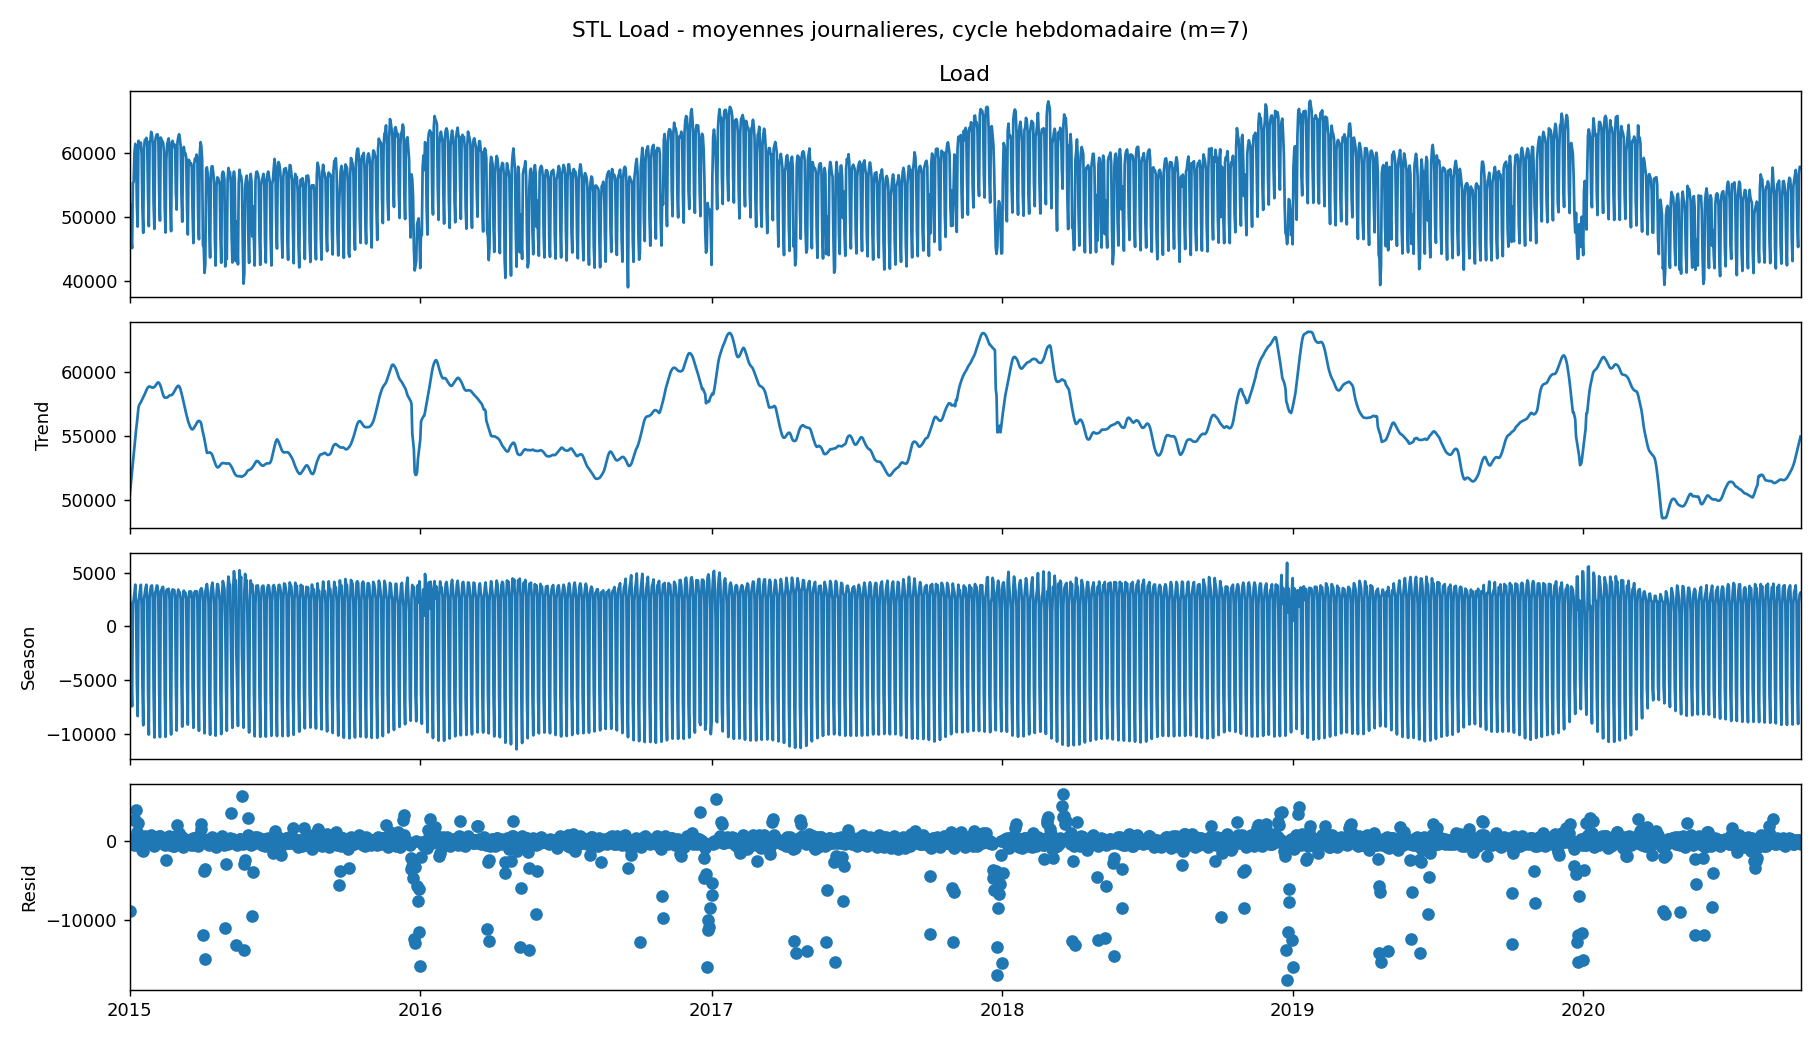
\includegraphics[width=0.75\textwidth]{py_stl_load_weekly.png}
\caption{Décomposition STL de la charge (cycle hebdomadaire).}
\label{fig:stl_weekly}
\end{figure}

\subsubsection{Valeurs manquantes et valeurs atypiques}
Les valeurs manquantes (figure~\ref{fig:missing_r} et~\ref{fig:missing_py})
sont rares et éparses. Le tableau~\ref{tab:outliers} montre que la règle IQR
globale ne détecte aucun point, tandis que la MAD roulante sur \(24\)~h
identifie \(761\) points atypiques (\(1{,}51\,\%\)) --- principalement des
épisodes éoliens extrêmes, illustrés par la figure~\ref{fig:outliers}.

\begin{figure}[H]
\centering
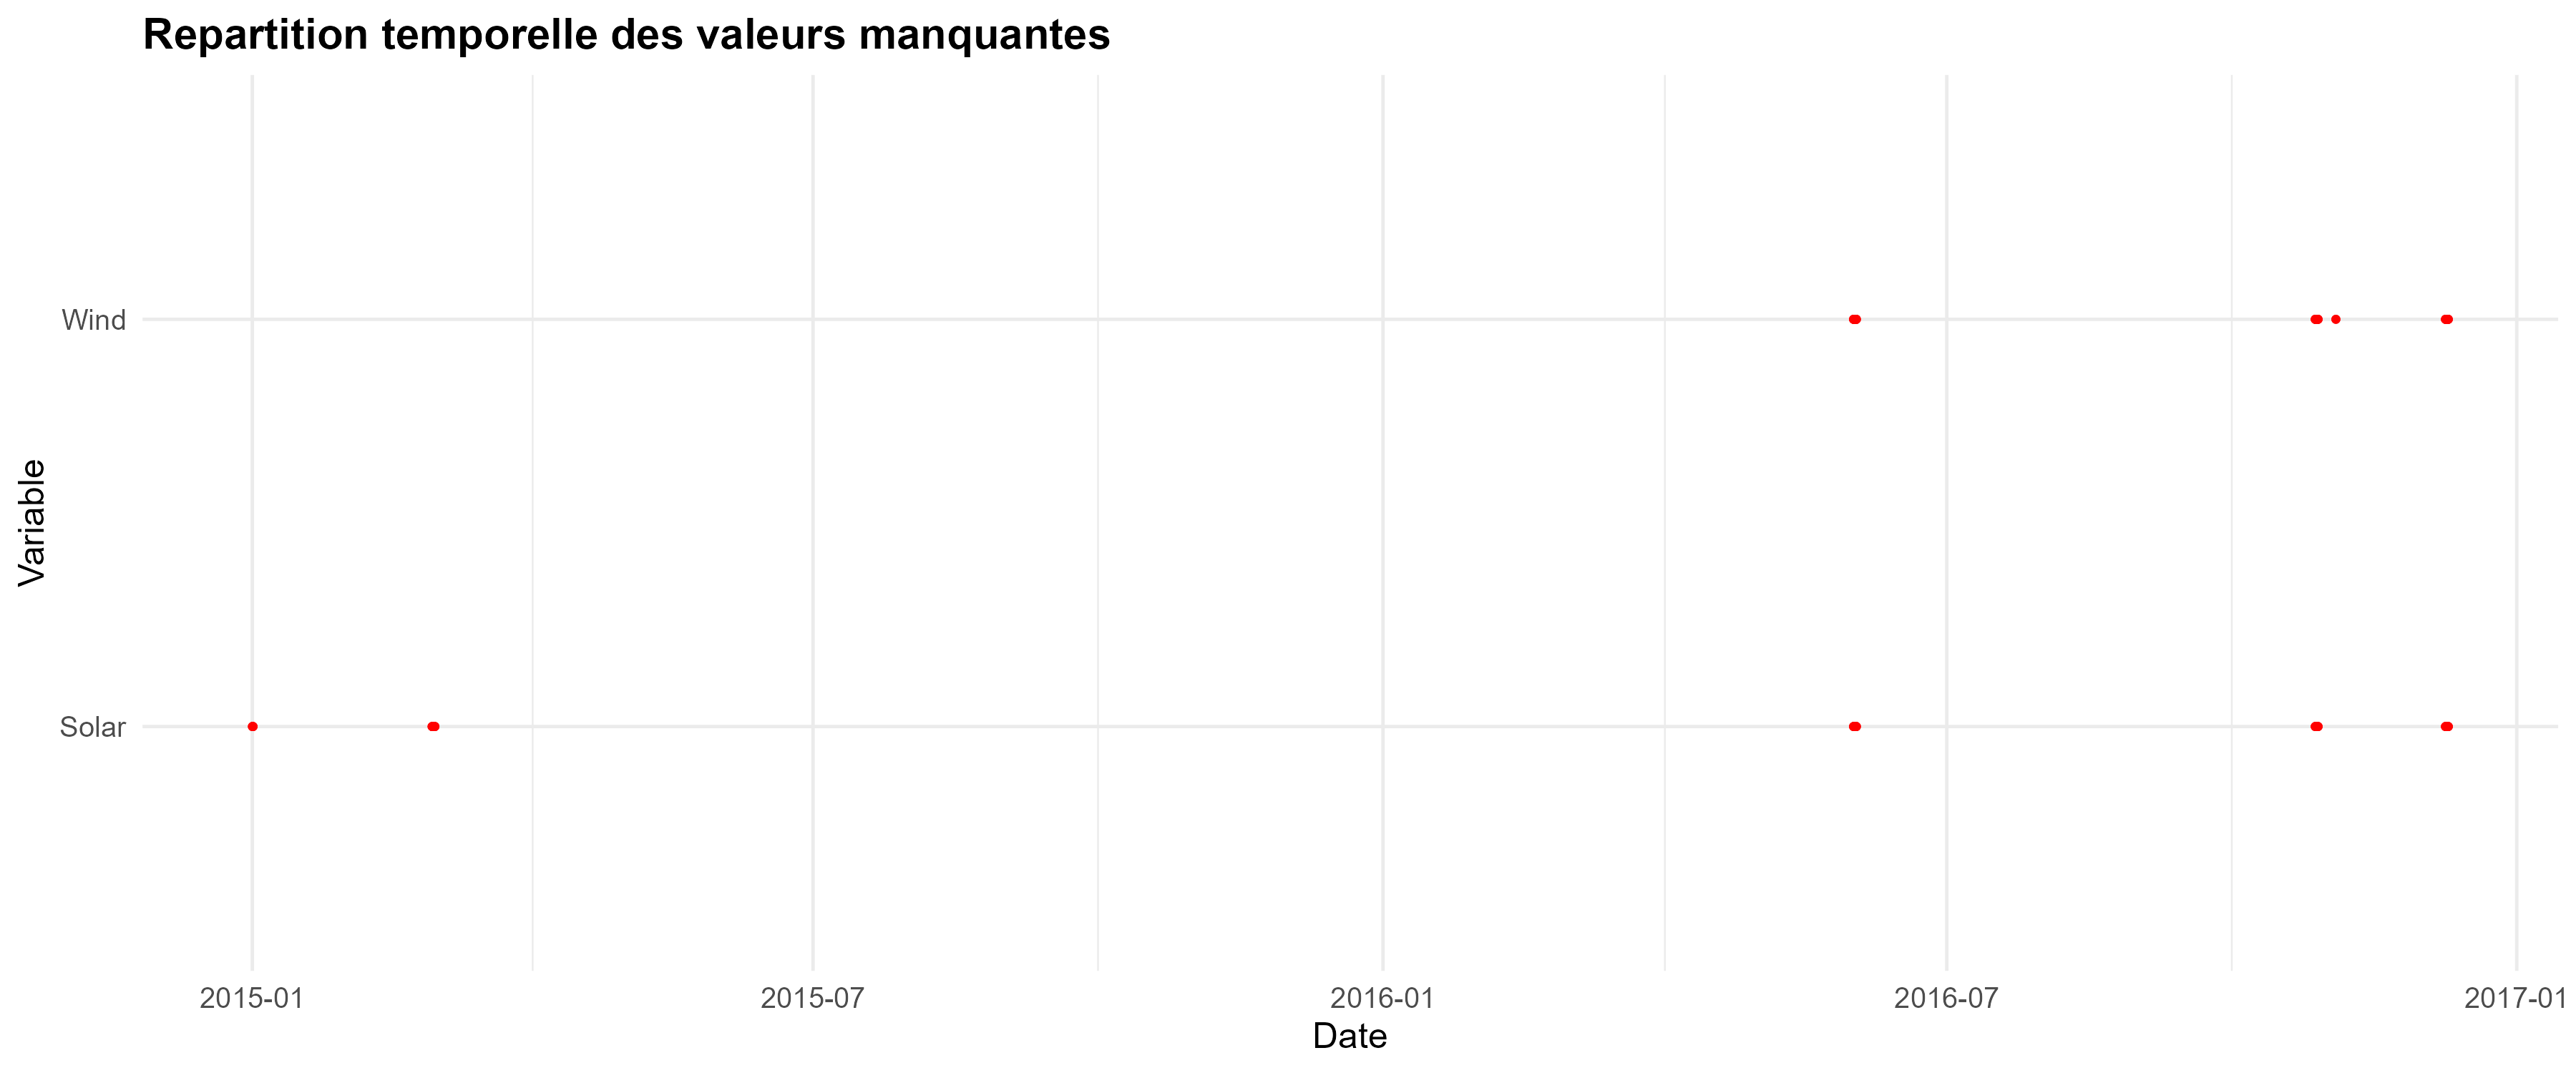
\includegraphics[width=0.9\textwidth]{missing_values.png}
\caption{Répartition temporelle des valeurs manquantes (R).}
\label{fig:missing_r}
\end{figure}

\begin{figure}[H]
\centering
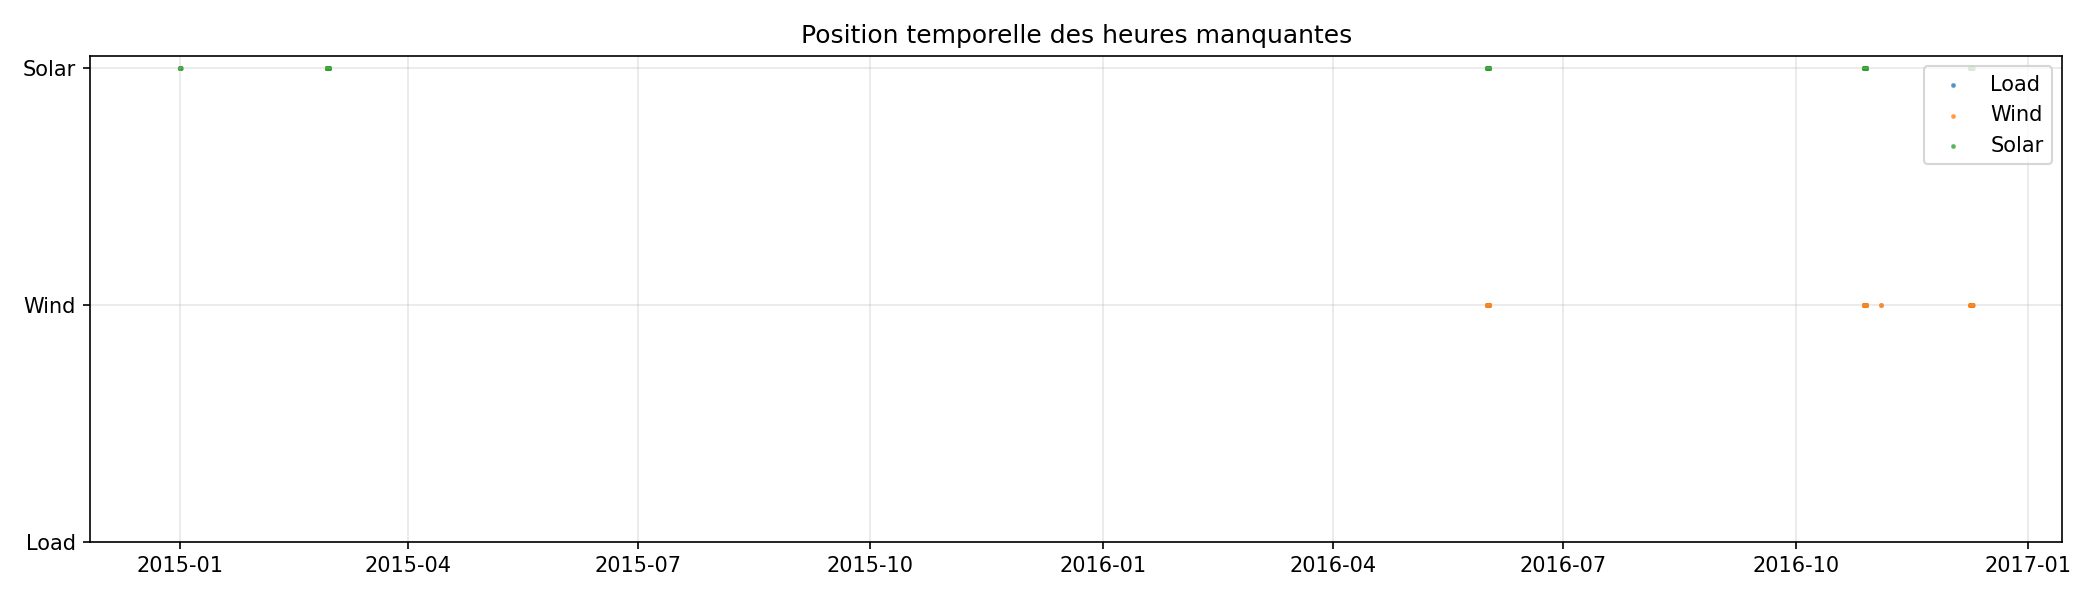
\includegraphics[width=0.9\textwidth]{py_missing.png}
\caption{Répartition temporelle des valeurs manquantes (Python).}
\label{fig:missing_py}
\end{figure}

\begin{table}[H]
\centering
\caption{Détection d'observations atypiques. Source : \texttt{outliers\_summary.csv}.}
\label{tab:outliers}
\begin{tabular}{lrr}
\toprule
Méthode & Nombre d'outliers & Part (\%) \\
\midrule
IQR global & 0 & 0{,}00 \\
MAD roulante 24~h & 761 & 1{,}51 \\
\bottomrule
\end{tabular}
\end{table}

\begin{figure}[H]
\centering
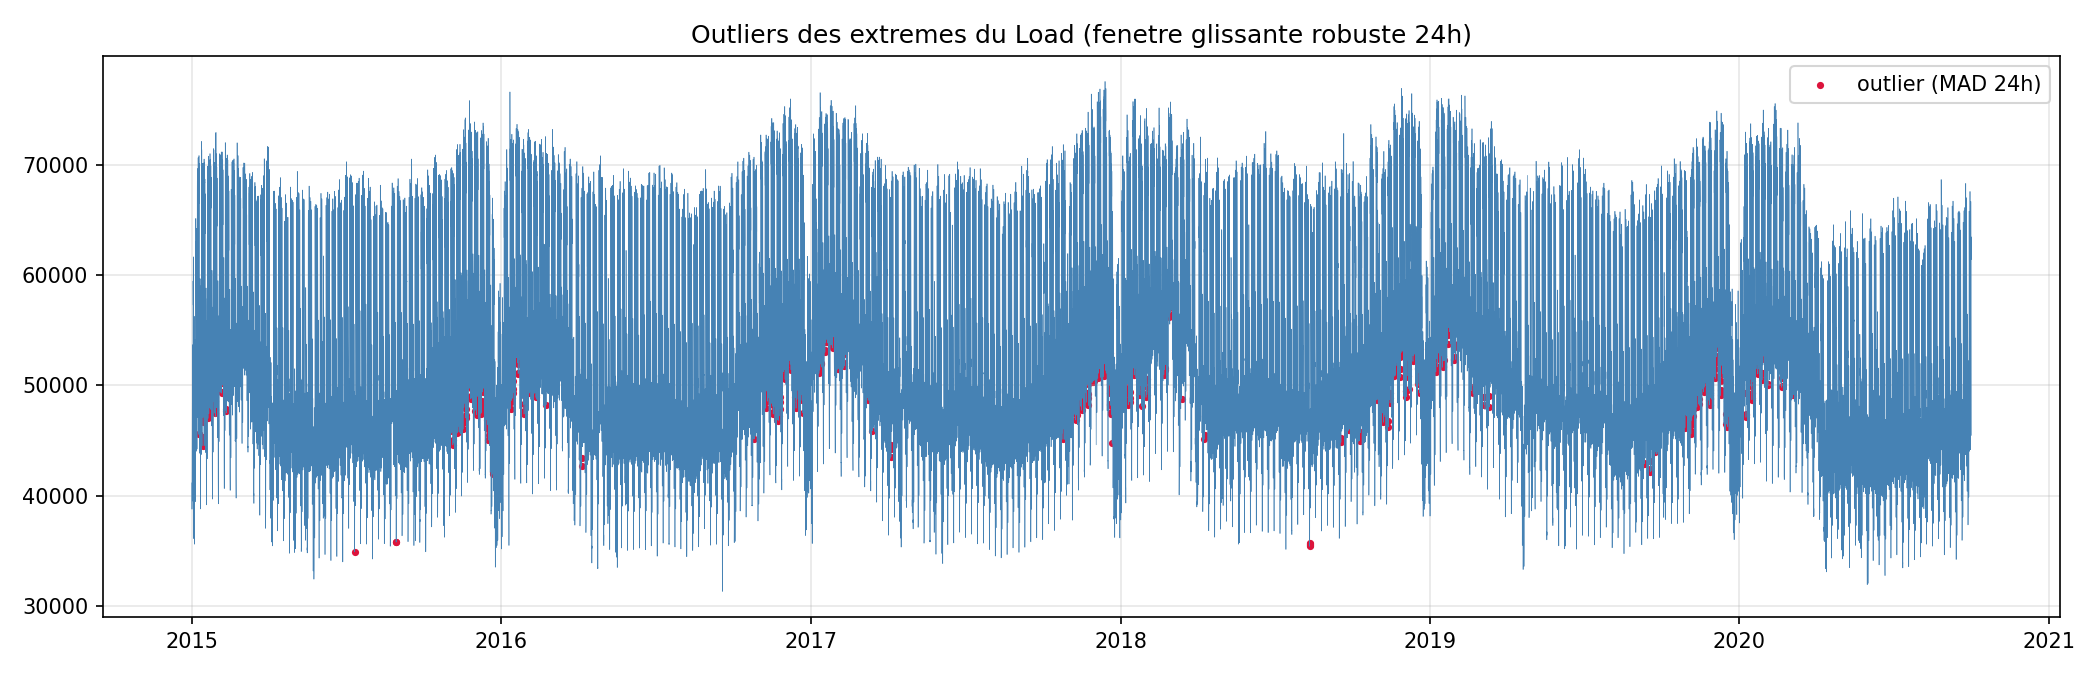
\includegraphics[width=0.85\textwidth]{py_outliers_load.png}
\caption{Détection d'outliers sur la charge (MAD roulante).}
\label{fig:outliers}
\end{figure}

\subsubsection{Stationnarité}
Le tableau~\ref{tab:stationnarite} (résultat R) montre que les séries brutes
sont jugées non stationnaires (ADF rejette la racine unitaire mais KPSS rejette
la stationnarité : les deux tests divergent). En différence première
(\(d=1\)), ADF et KPSS s'accordent : les séries sont \textbf{stationnaires}.
Ceci justifie l'usage de \(d=1\) dans les modèles ARIMA et de \(D1\) dans le
VAR/GARCH. Les conclusions sont identiques côté Python
(\texttt{stationarity\_tests.csv}).

\begin{table}[H]
\centering
\caption{Tests de stationnarité ADF / KPSS (R). Source : \texttt{R\_stationarity\_tests.csv}.}
\label{tab:stationnarite}
\small
\begin{tabular}{llrrrrl}
\toprule
Variable & Transf. & ADF stat & ADF p & KPSS stat & KPSS p & Stationnaire ? \\
\midrule
\texttt{Load}  & brute & $-24{,}75$ & 0{,}01 & 2{,}497 & 0{,}01 & Non \\
\texttt{Load}  & $d1$  & $-42{,}49$ & 0{,}01 & 0{,}0007 & 0{,}10 & Oui \\
\texttt{Wind}  & brute & $-18{,}68$ & 0{,}01 & 17{,}363 & 0{,}01 & Non \\
\texttt{Wind}  & $d1$  & $-44{,}68$ & 0{,}01 & 0{,}0005 & 0{,}10 & Oui \\
\texttt{Solar} & brute & $-11{,}69$ & 0{,}01 & 10{,}792 & 0{,}01 & Non \\
\texttt{Solar} & $d1$  & $-46{,}02$ & 0{,}01 & 0{,}0004 & 0{,}10 & Oui \\
\bottomrule
\end{tabular}
\end{table}

\subsubsection{Corrélogrammes ACF / PACF}
Les figures~\ref{fig:acf_load_raw} à~\ref{fig:acf_solar_d1} présentent les
ACF/PACF (R puis Python). Les séries brutes affichent une décroissance lente
et des rebonds marqués à \(24\) et \(168\) (saisonnalité quotidienne et
hebdomadaire). Après différenciation, les autocorrélations restent
significatives aux retards saisonniers, motivant la composante saisonnière
\((1,1,1)_{24}\).

\begin{figure}[H]
\centering
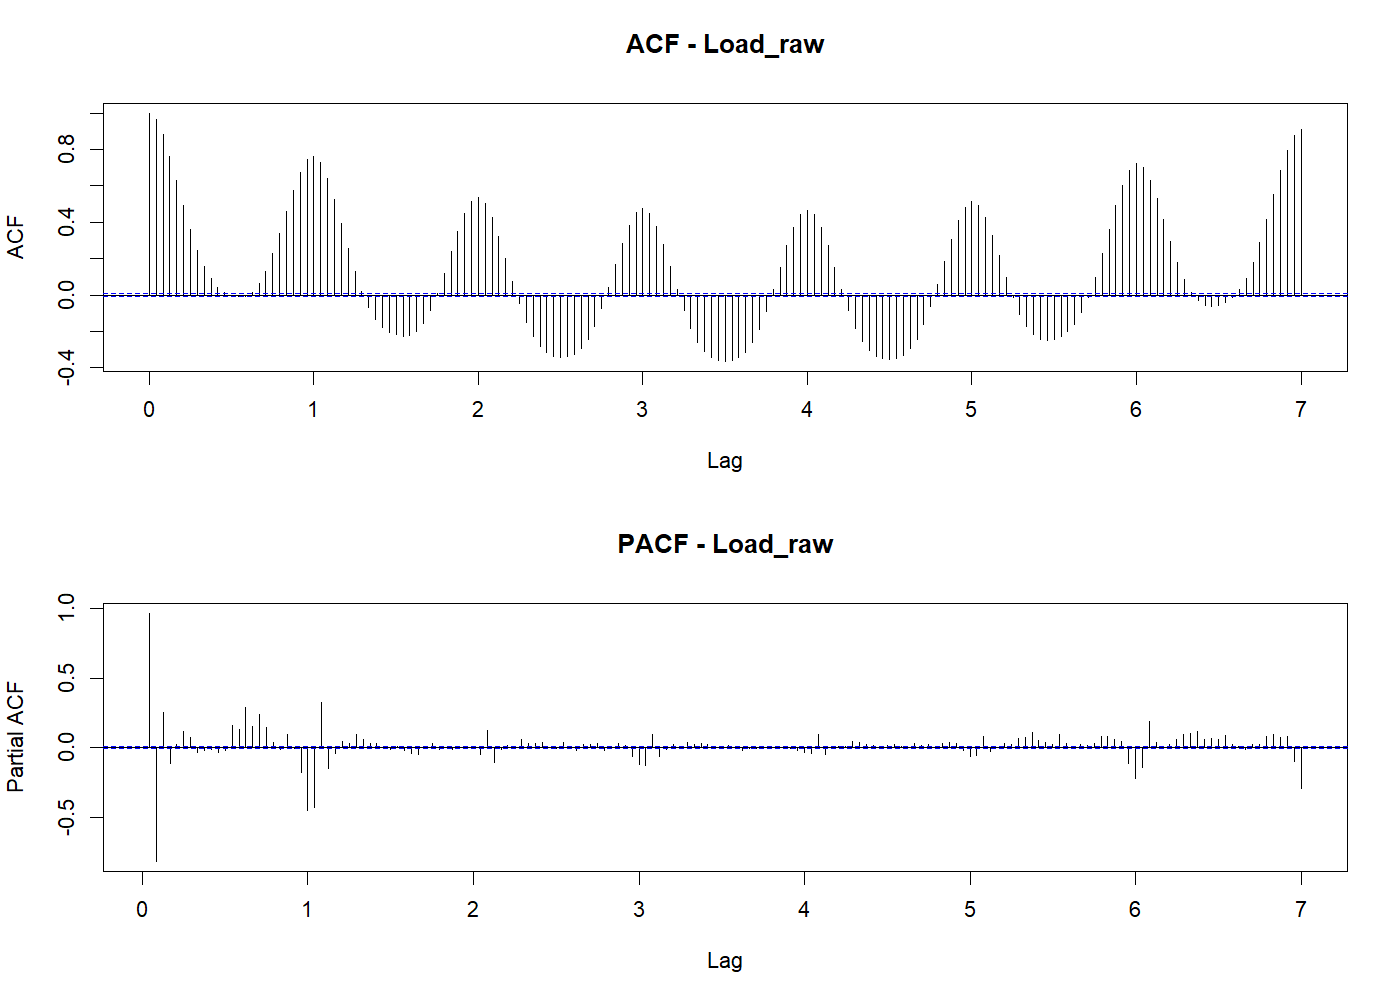
\includegraphics[width=0.95\textwidth]{R_acf_pacf_Load_raw.png}
\caption{ACF/PACF de \texttt{Load} (série brute, R).}
\label{fig:acf_load_raw}
\end{figure}

\begin{figure}[H]
\centering
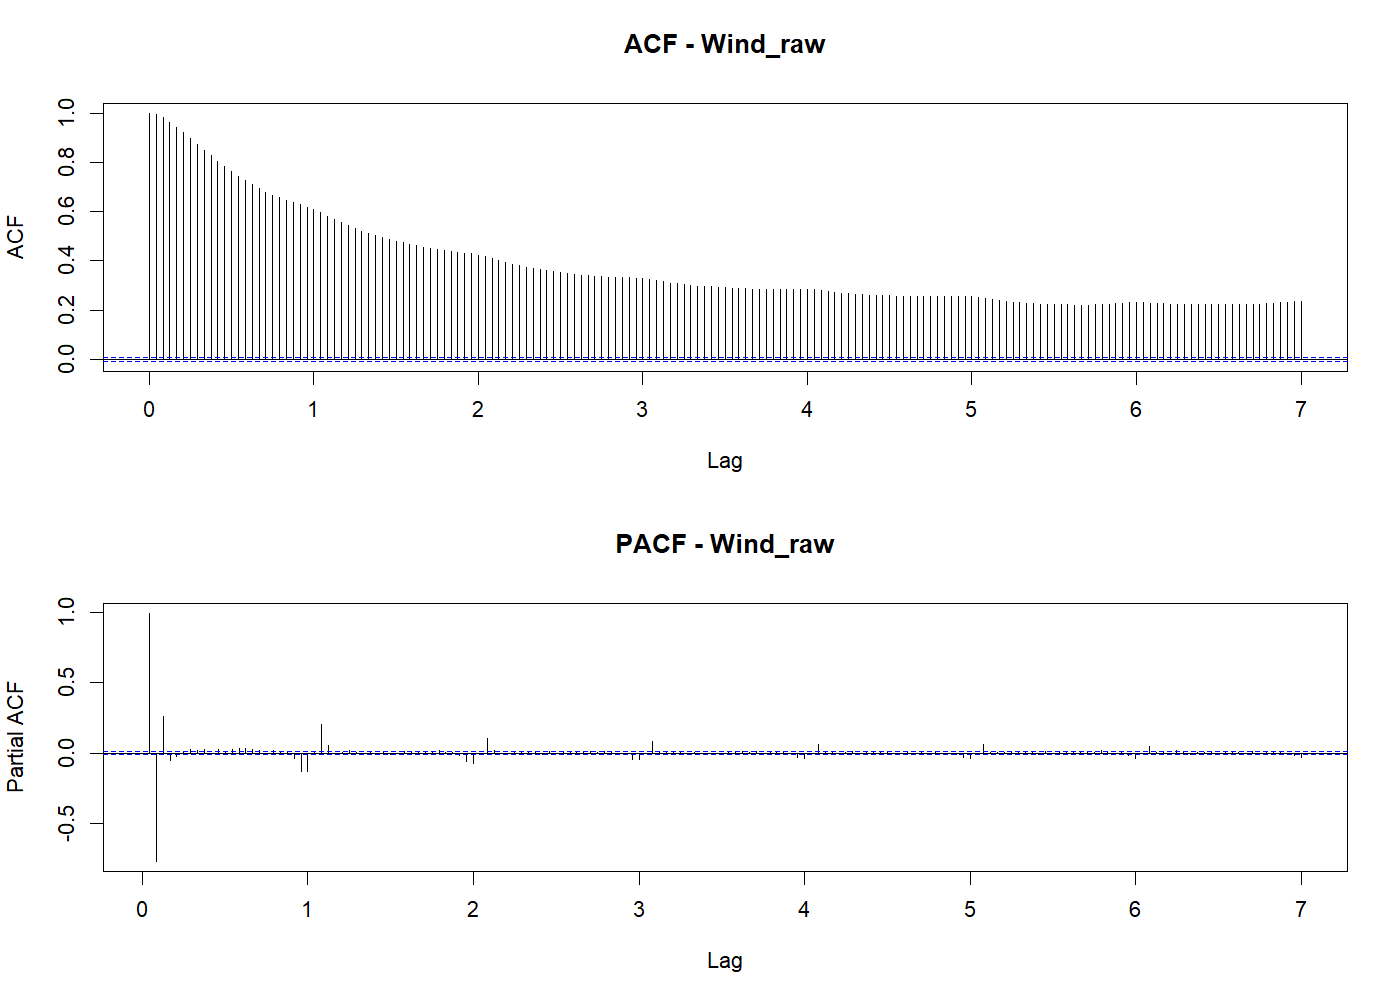
\includegraphics[width=0.95\textwidth]{R_acf_pacf_Wind_raw.png}
\caption{ACF/PACF de \texttt{Wind} (série brute, R).}
\label{fig:acf_wind_raw}
\end{figure}

\begin{figure}[H]
\centering
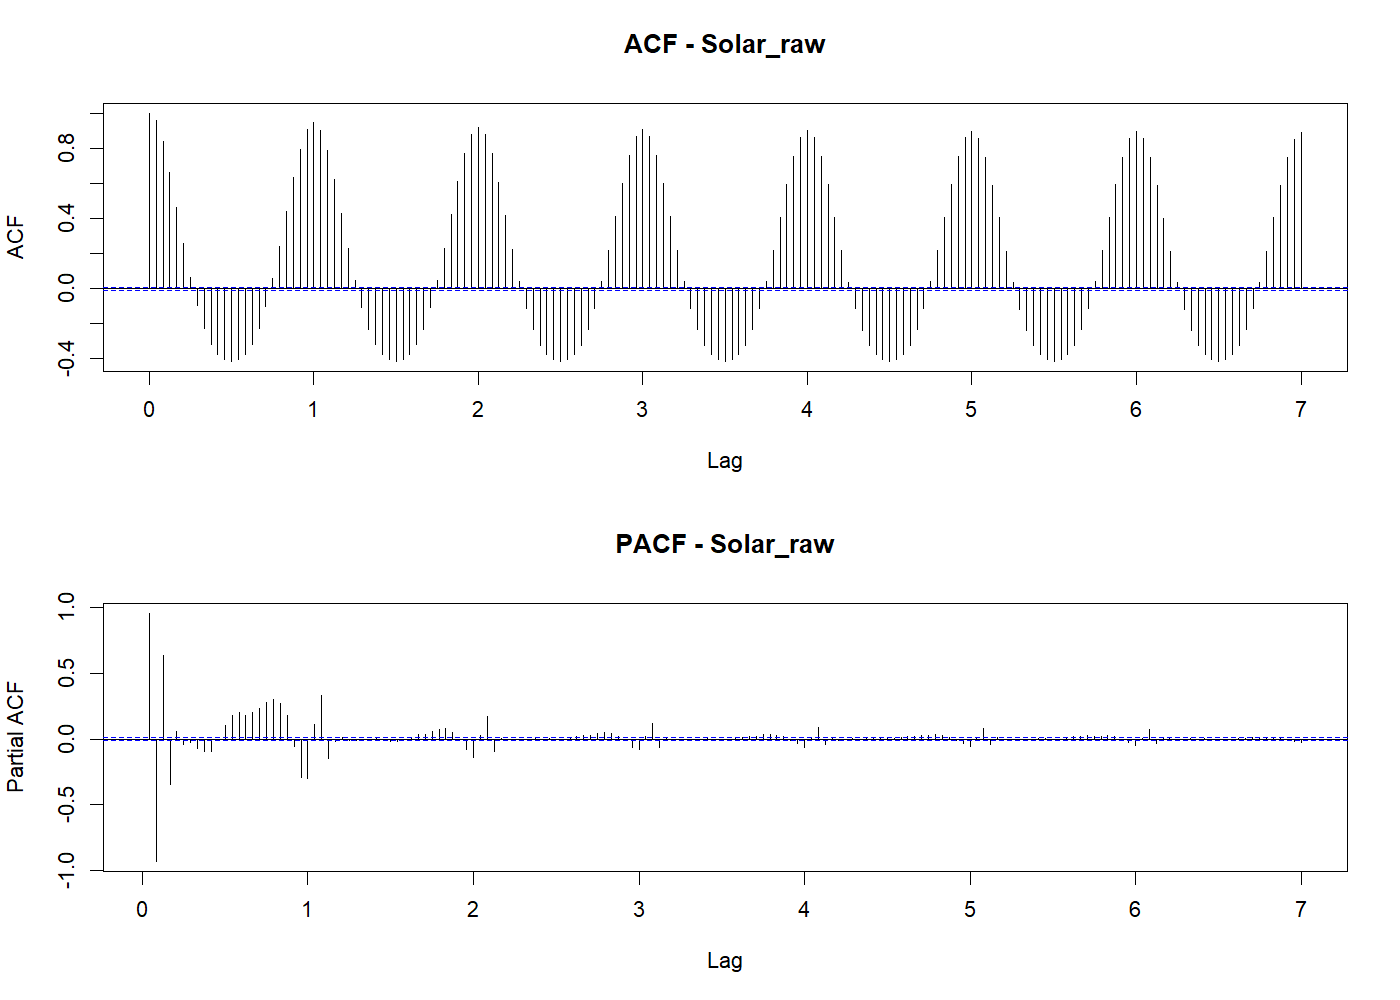
\includegraphics[width=0.95\textwidth]{R_acf_pacf_Solar_raw.png}
\caption{ACF/PACF de \texttt{Solar} (série brute, R).}
\label{fig:acf_solar_raw}
\end{figure}

\begin{figure}[H]
\centering
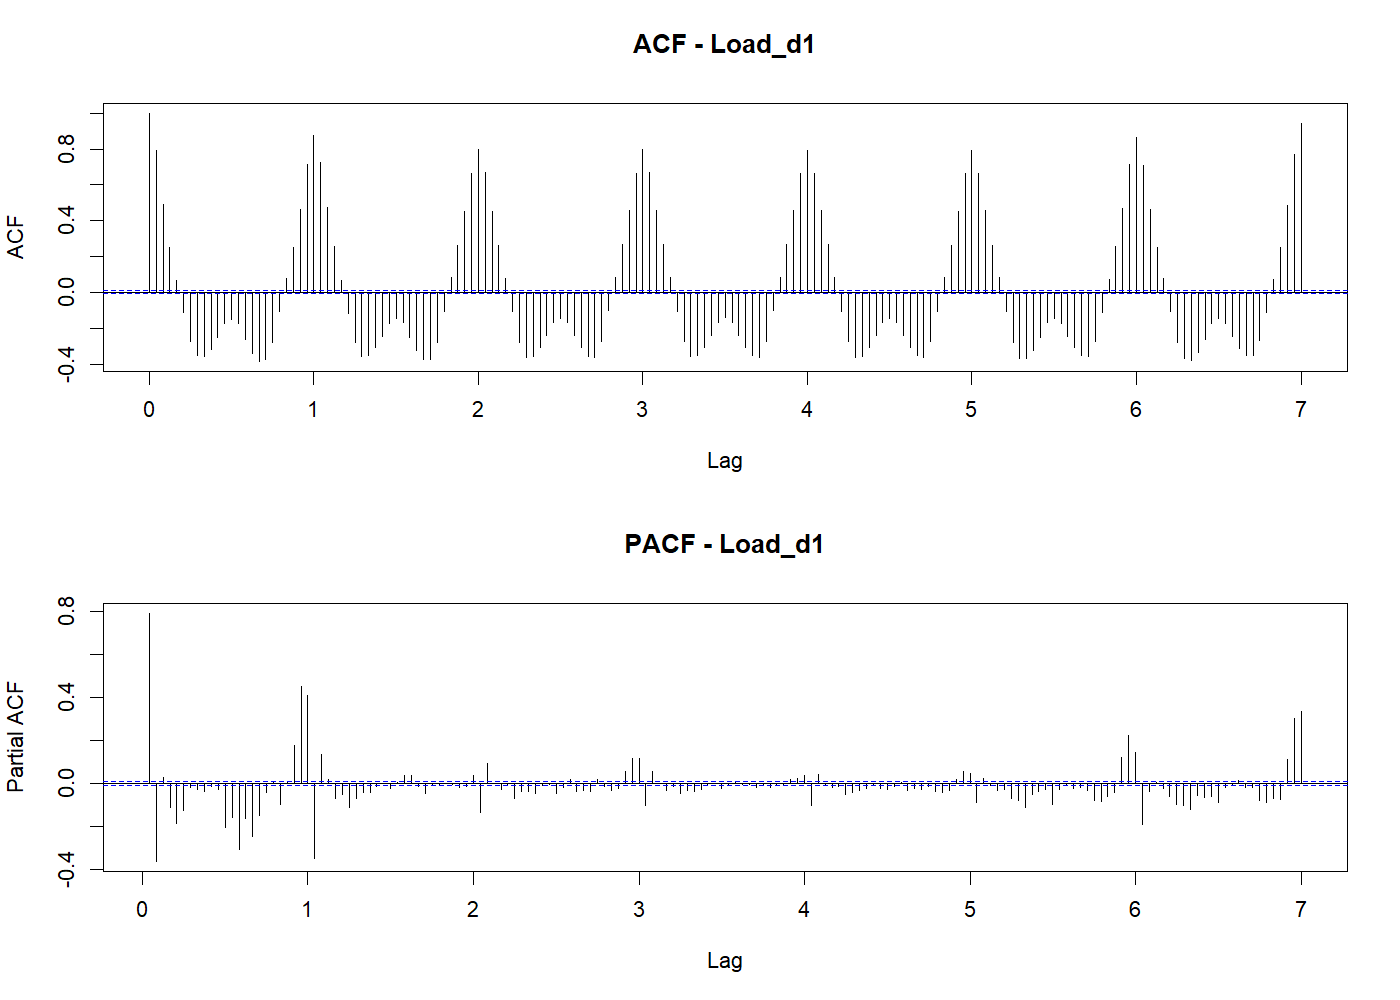
\includegraphics[width=0.95\textwidth]{R_acf_pacf_Load_d1.png}
\caption{ACF/PACF de \texttt{Load} différenciée ($d1$, R).}
\label{fig:acf_load_d1}
\end{figure}

\begin{figure}[H]
\centering
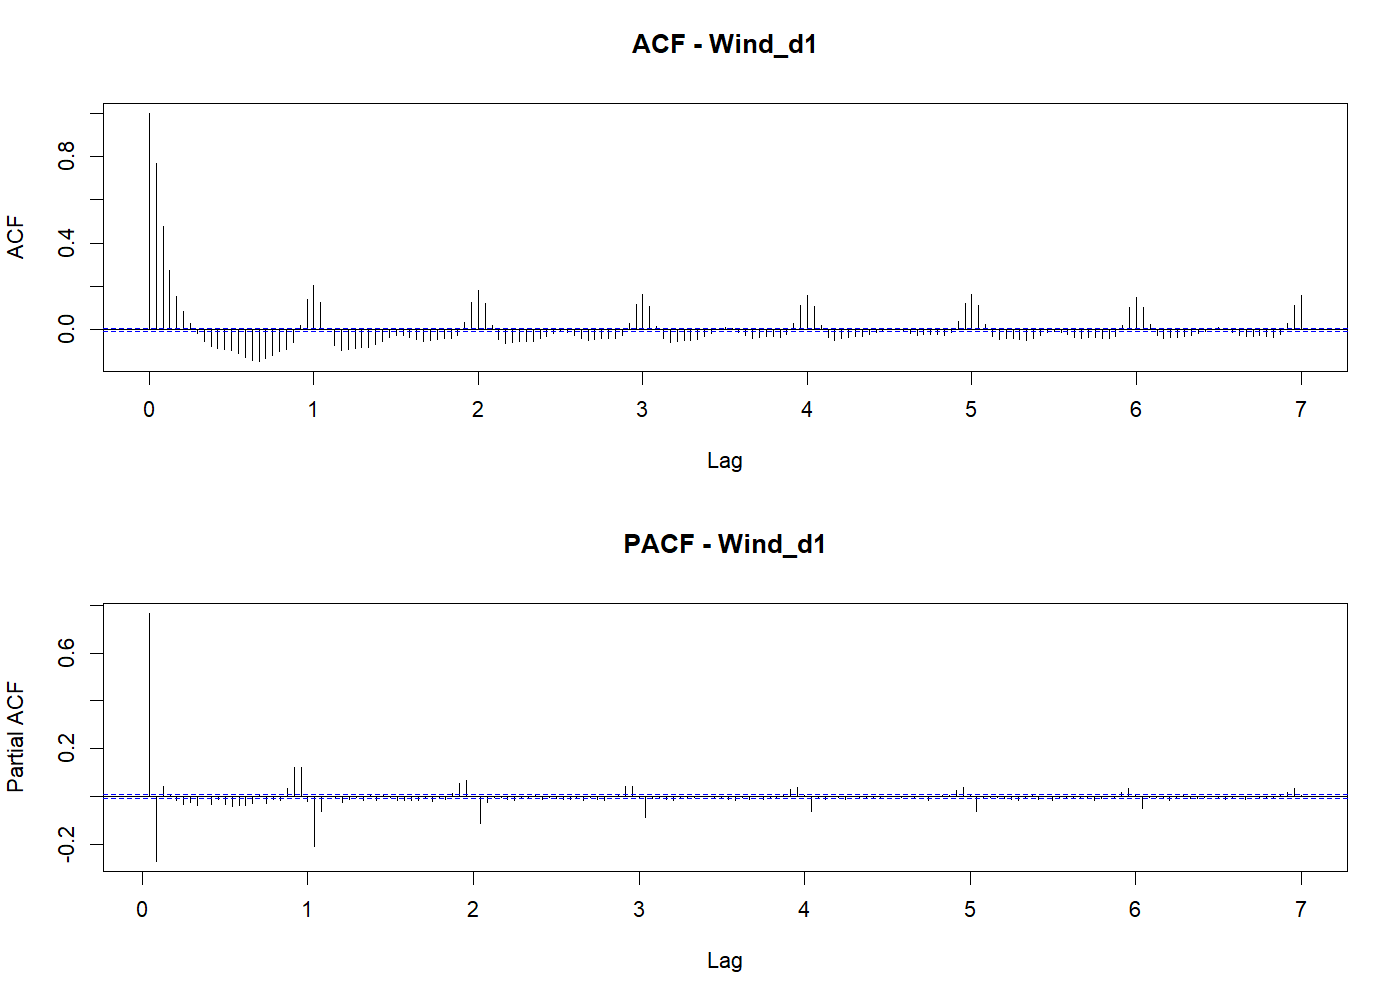
\includegraphics[width=0.95\textwidth]{R_acf_pacf_Wind_d1.png}
\caption{ACF/PACF de \texttt{Wind} différenciée ($d1$, R).}
\label{fig:acf_wind_d1}
\end{figure}

\begin{figure}[H]
\centering
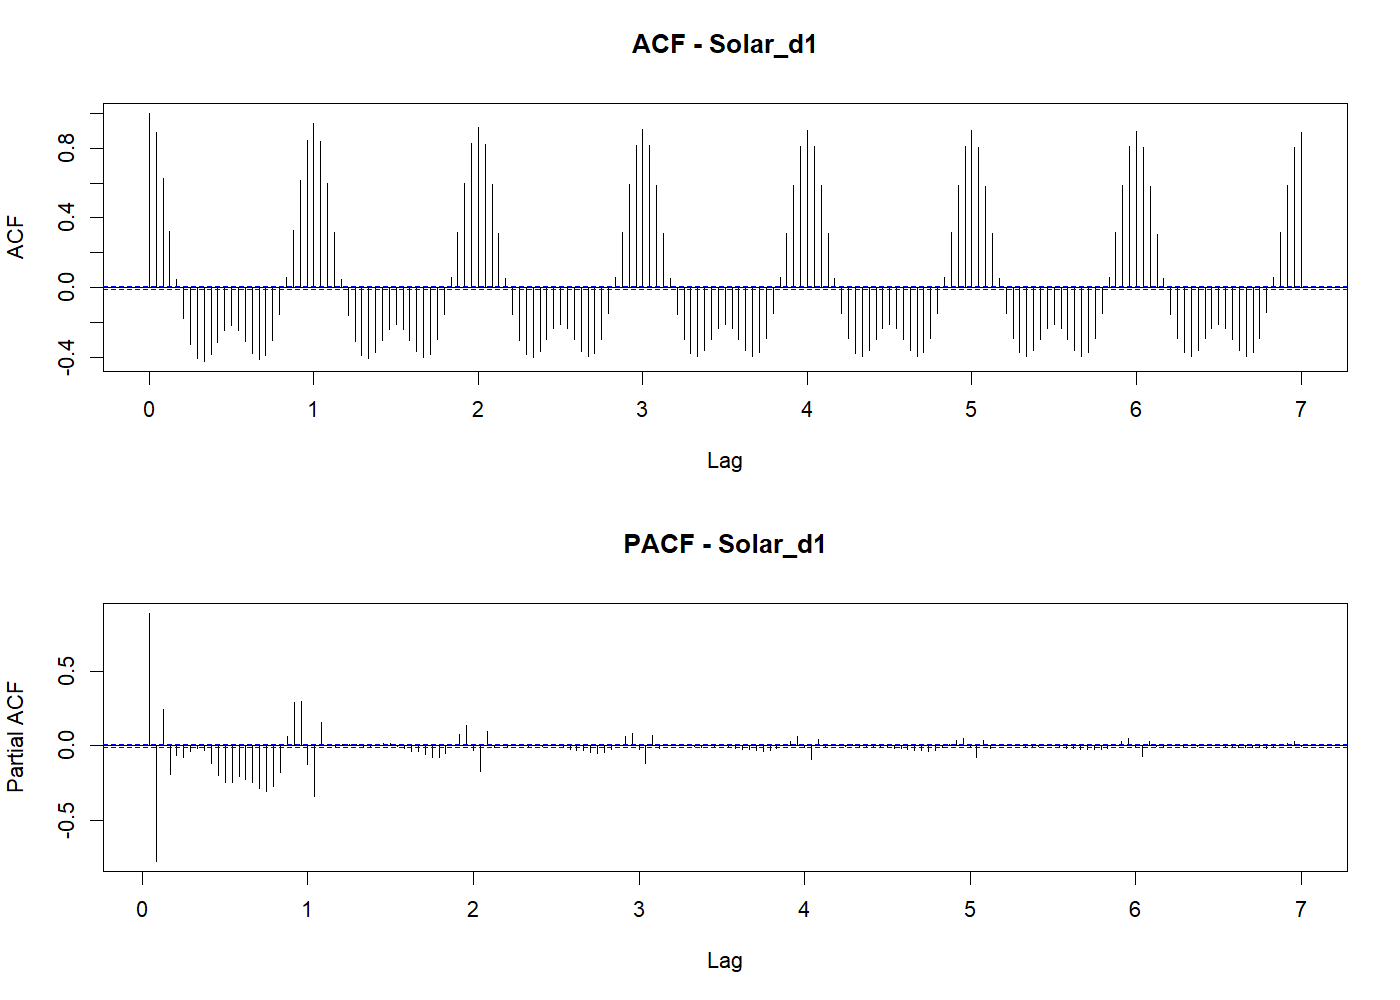
\includegraphics[width=0.95\textwidth]{R_acf_pacf_Solar_d1.png}
\caption{ACF/PACF de \texttt{Solar} différenciée ($d1$, R).}
\label{fig:acf_solar_d1}
\end{figure}

\begin{figure}[H]
\centering
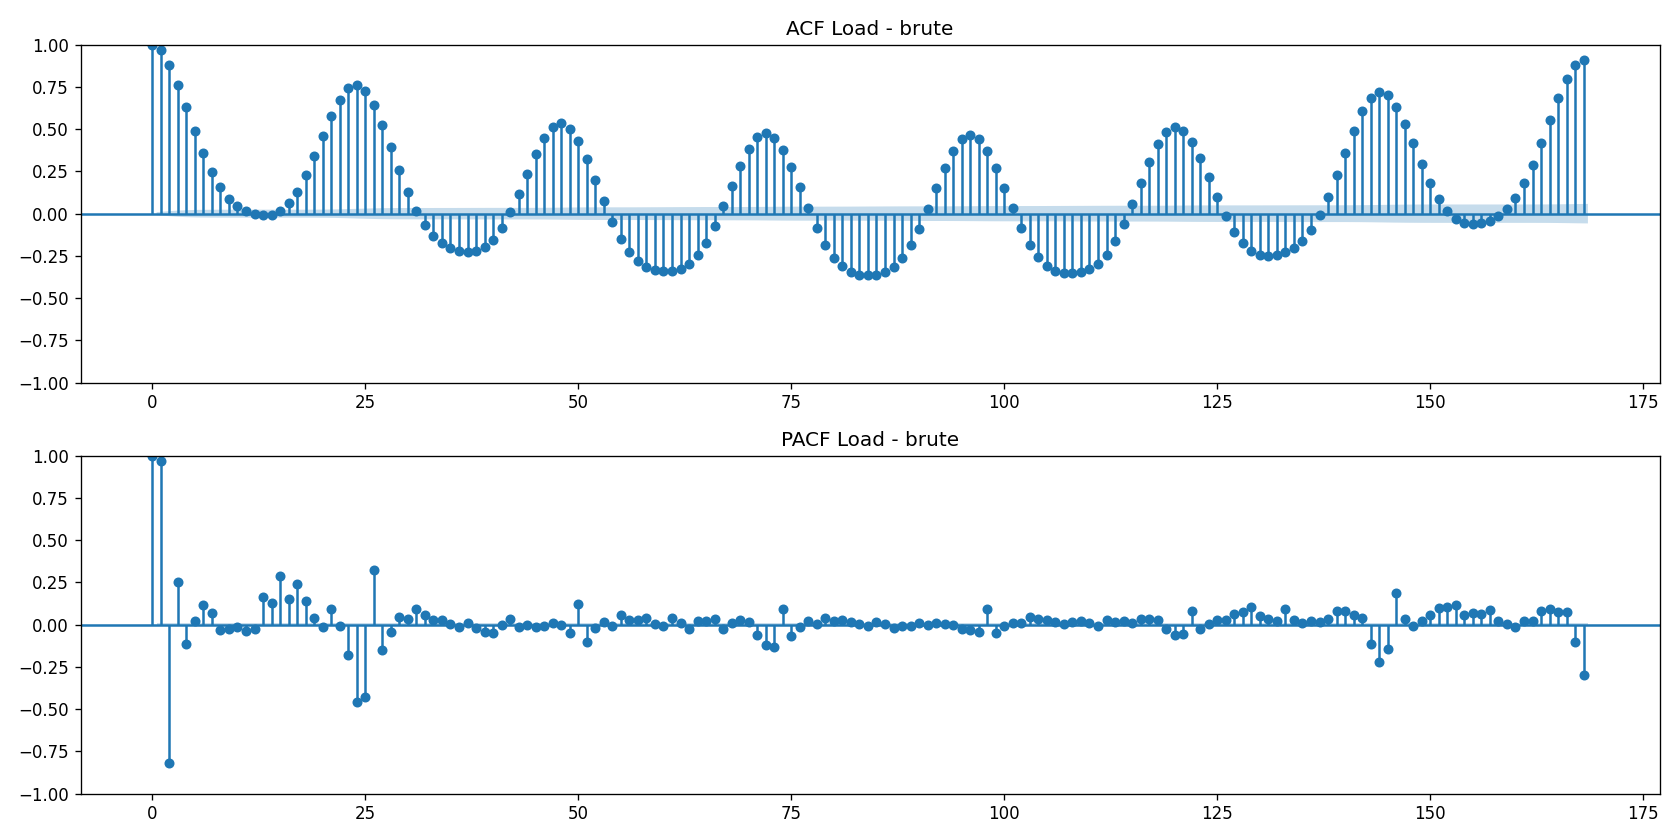
\includegraphics[width=0.8\textwidth]{py_acf_pacf_Load_raw.png}
\caption{ACF/PACF de \texttt{Load} brute (Python). À comparer avec la
figure~\ref{fig:acf_load_raw}.}
\label{fig:acf_py_load}
\end{figure}

\begin{figure}[H]
\centering
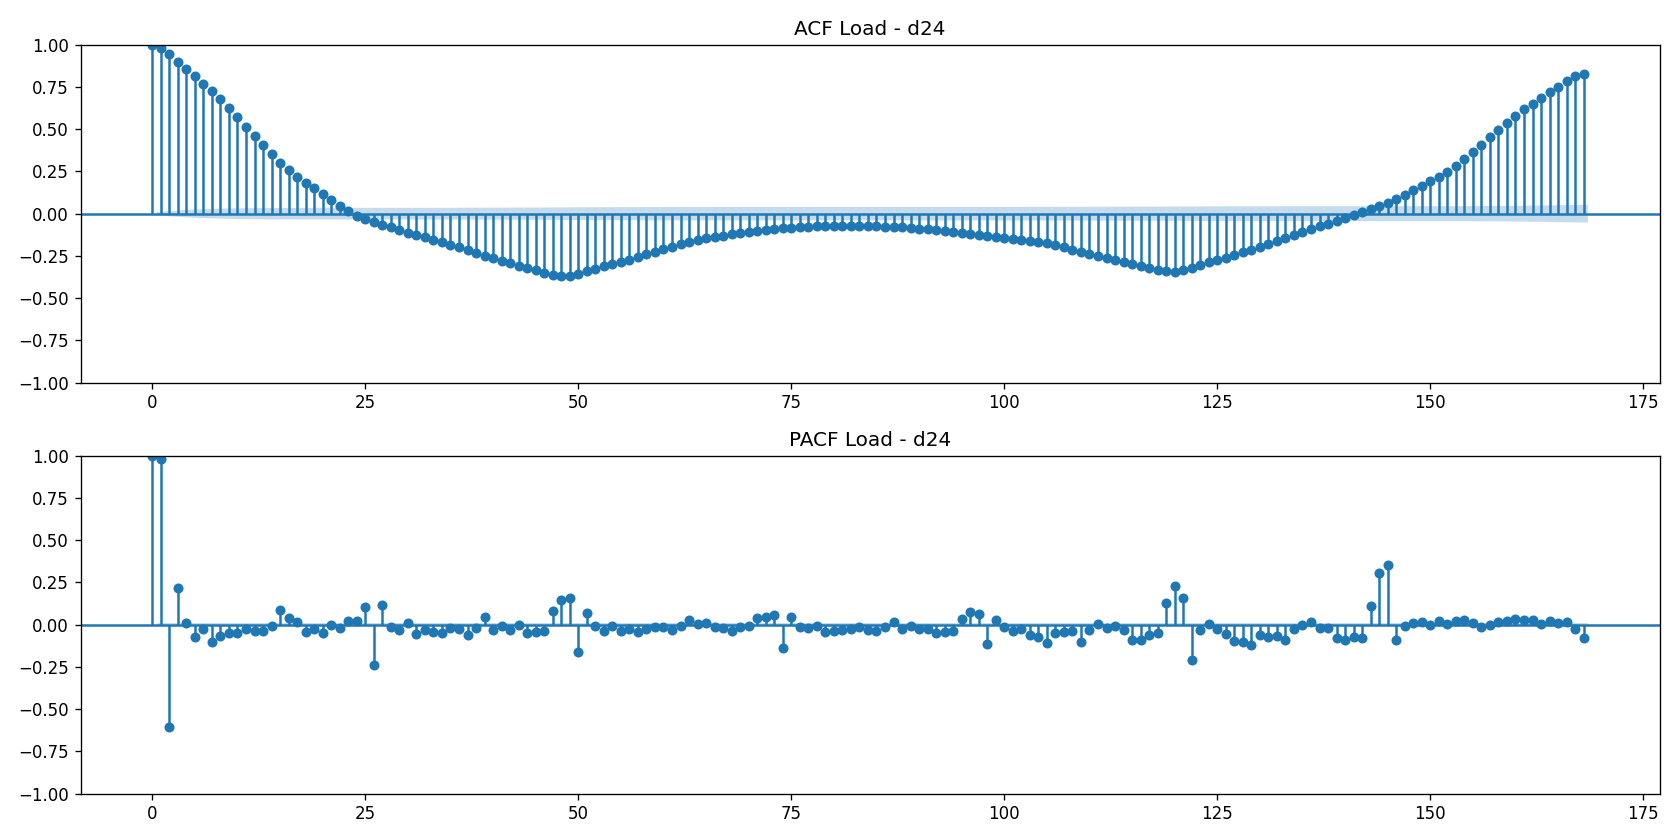
\includegraphics[width=0.95\textwidth]{py_acf_pacf_Load_d24.png}
\caption{ACF/PACF de \texttt{Load} en différence saisonnière ($d24$, Python).}
\label{fig:acf_py_load_d24}
\end{figure}

\begin{figure}[H]
\centering
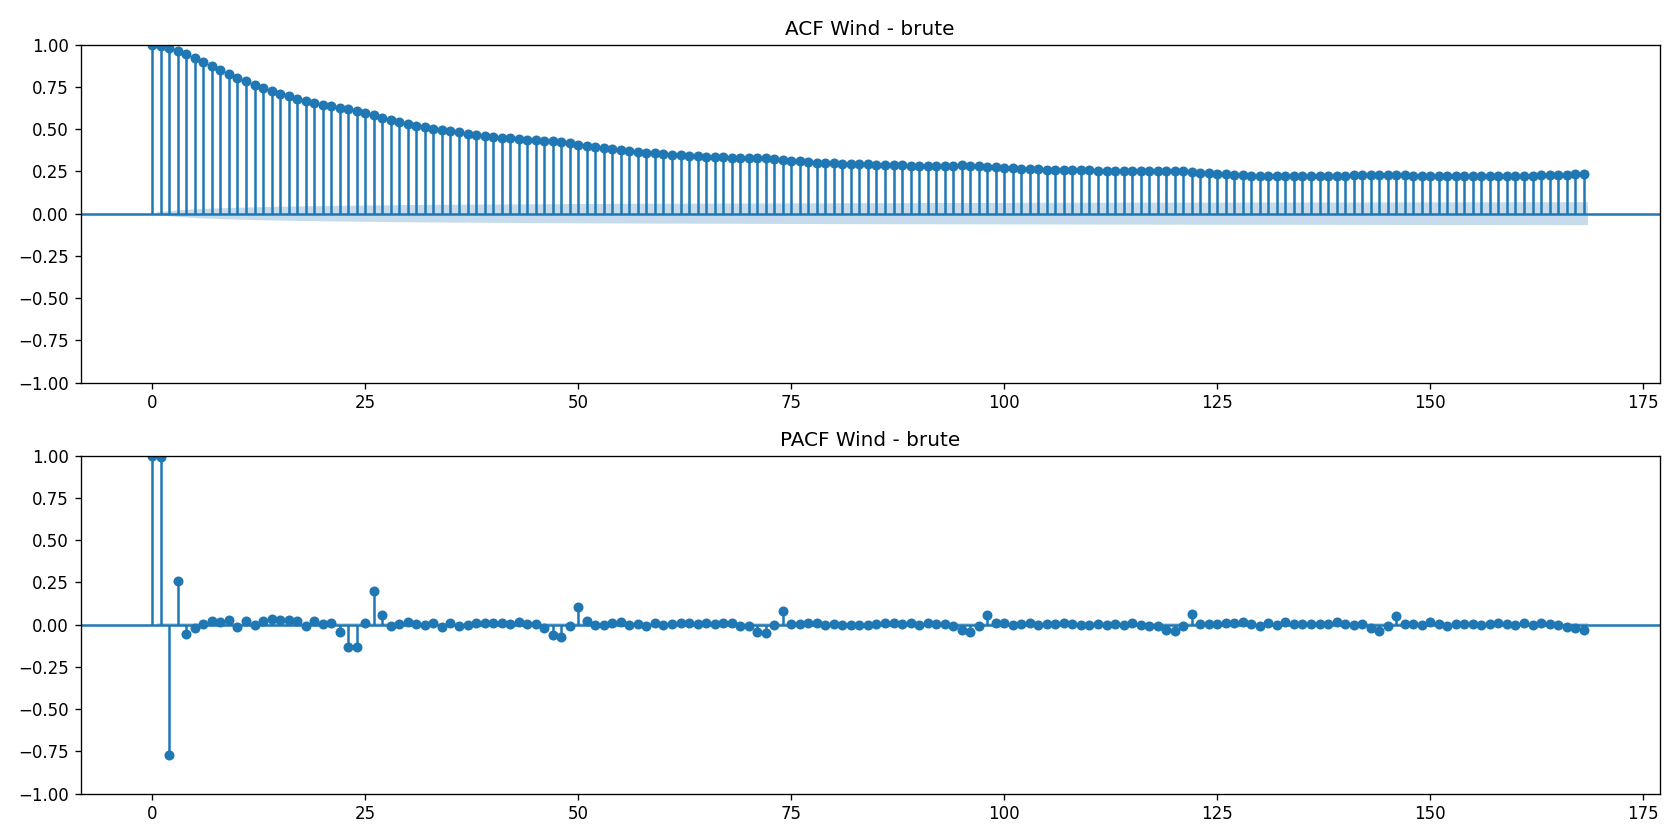
\includegraphics[width=0.95\textwidth]{py_acf_pacf_Wind_raw.png}
\caption{ACF/PACF de \texttt{Wind} brute (Python).}
\label{fig:acf_py_wind}
\end{figure}

\begin{figure}[H]
\centering
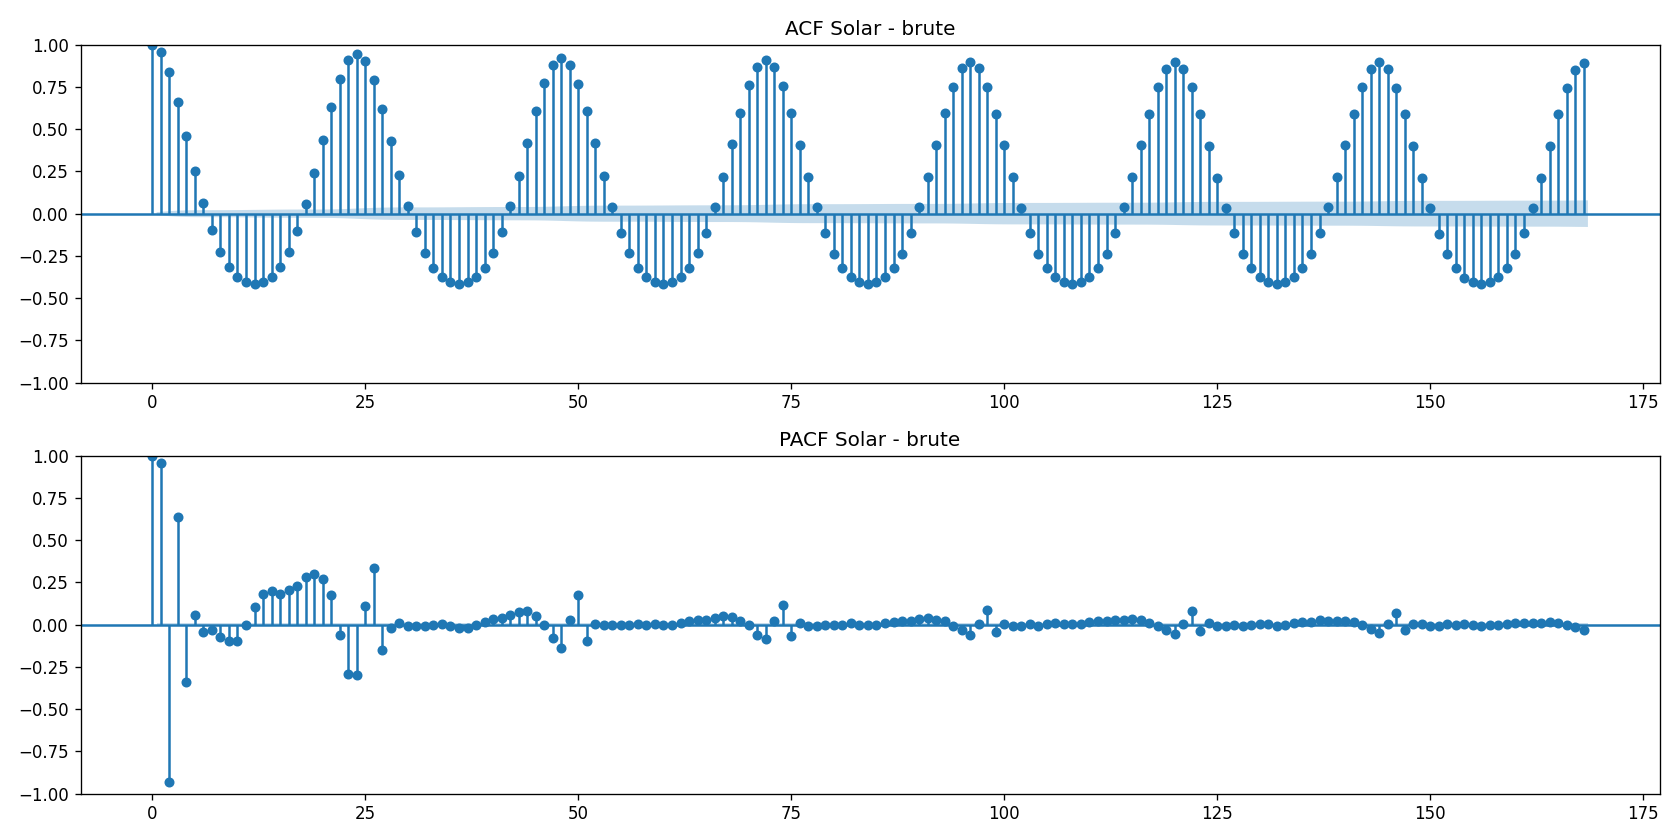
\includegraphics[width=0.95\textwidth]{py_acf_pacf_Solar_raw.png}
\caption{ACF/PACF de \texttt{Solar} brute (Python).}
\label{fig:acf_py_solar}
\end{figure}

\FloatBarrier

\subsection{Socle univarié : ARIMA / SARIMA}

\subsubsection{Sélection des modèles}
Le tableau~\ref{tab:arima_comp_r} (R) et le tableau~\ref{tab:arima_comp_py}
(Python) comparent les trois candidats par AIC/AICc/BIC. Les deux
implémentations retiennent des ordres \textbf{identiques} :
\begin{itemize}
  \item \texttt{Load} : \texttt{SARIMA\_manuel} \(\text{ARIMA}(1,1,1)(1,1,1)_{24}\)
        (AICc minimal) ;
  \item \texttt{Wind} : \texttt{SARIMA\_manuel} également retenu ;
  \item \texttt{Solar} : \texttt{SARIMA\_auto} \(\text{ARIMA}(2,1,2)(0,1,1)_{24}\)
        au plus faible AICc.
\end{itemize}
Le modèle non saisonnier \texttt{ARIMA\_auto} présente systématiquement un
AICc nettement supérieur, confirmant la nécessité de la composante saisonnière
\(m=24\).

\begin{table}[H]
\centering
\caption{Comparaison des modèles ARIMA/SARIMA (R). AICc minimal en gras.
Source : \texttt{R\_arima\_model\_comparison.csv}.}
\label{tab:arima_comp_r}
\small
\begin{tabular}{llrrrl}
\toprule
Variable & Modèle & AIC & AICc & BIC & Spécification \\
\midrule
\texttt{Load}  & SARIMA\_manuel & 740\,406 & \textbf{740\,406{,}22} & 740\,450 & ARIMA(1,1,1)(1,1,1)[24] \\
\texttt{Load}  & ARIMA\_auto    & 786\,041 & 786\,041{,}00 & 786\,102 & ARIMA(5,1,1) \\
\texttt{Load}  & SARIMA\_auto   & 752\,342 & 752\,341{,}81 & 752\,394 & ARIMA(2,1,2)(1,1,0)[24] \\
\texttt{Wind}  & SARIMA\_manuel & 694\,884 & \textbf{694\,884{,}46} & 694\,928 & ARIMA(1,1,1)(1,1,1)[24] \\
\texttt{Wind}  & ARIMA\_auto    & 701\,054 & 701\,054{,}37 & 701\,115 & ARIMA(2,1,3) \\
\texttt{Wind}  & SARIMA\_auto   & 698\,594 & 698\,594{,}09 & 698\,638 & ARIMA(1,1,2)(1,0,0)[24] \\
\texttt{Solar} & SARIMA\_manuel & 656\,144 & 656\,143{,}85 & 656\,187 & ARIMA(1,1,1)(1,1,1)[24] \\
\texttt{Solar} & ARIMA\_auto    & 700\,943 & 700\,943{,}17 & 700\,987 & ARIMA(2,1,2) \\
\texttt{Solar} & SARIMA\_auto   & 650\,435 & \textbf{650\,434{,}88} & 650\,487 & ARIMA(2,1,2)(0,1,1)[24] \\
\bottomrule
\end{tabular}
\end{table}

\begin{table}[H]
\centering
\caption{Comparaison des modèles ARIMA/SARIMA (Python) --- confirme les ordres
retenus en R. Source : \texttt{py\_arima\_model\_comparison.csv}.}
\label{tab:arima_comp_py}
\small
\begin{tabular}{llrrrl}
\toprule
Variable & Modèle & AIC & AICc & BIC & Spécification \\
\midrule
\texttt{Load}  & SARIMA\_manuel & 739\,990 & 739\,990 & 740\,033 & ARIMA(1,1,1)(1,1,1)[24] \\
\texttt{Load}  & ARIMA\_auto    & 786\,510 & 786\,510 & 786\,571 & ARIMA(5,1,1) \\
\texttt{Load}  & SARIMA\_auto   & 752\,042 & 752\,042 & 752\,095 & ARIMA(2,1,2)(1,1,0)[24] \\
\texttt{Wind}  & ARIMA\_auto    & 701\,099 & 701\,099 & 701\,152 & ARIMA(2,1,3) \\
\texttt{Wind}  & SARIMA\_auto   & 698\,280 & 698\,280 & 698\,324 & ARIMA(1,1,2)(1,0,0)[24] \\
\texttt{Solar} & SARIMA\_manuel & 655\,665 & 655\,665 & 655\,709 & ARIMA(1,1,1)(1,1,1)[24] \\
\texttt{Solar} & ARIMA\_auto    & 701\,059 & 701\,059 & 701\,103 & ARIMA(2,1,2) \\
\texttt{Solar} & SARIMA\_auto   & 649\,997 & 649\,997 & 650\,049 & ARIMA(2,1,2)(0,1,1)[24] \\
\bottomrule
\end{tabular}
\end{table}

\subsubsection{Diagnostics des résidus}
Le tableau~\ref{tab:arima_diag} présente les diagnostics du meilleur modèle
par série. Quelle que soit l'implémentation, les trois tests rejettent leurs
hypothèses nulles : autocorrélation résiduelle partielle (Ljung--Box),
non-normalité (Jarque--Bera) et surtout \textbf{effet ARCH persistant}
(ARCH--LM), ce dernier point justifiant directement le volet GARCH
(section~\ref{sec:garch}).

\begin{table}[H]
\centering
\caption{Diagnostics des résidus du meilleur modèle ARIMA/SARIMA.
Sources : \texttt{R\_arima\_diagnostics.csv} et \texttt{py\_arima\_diagnostics.csv}.}
\label{tab:arima_diag}
\small
\begin{tabular}{llrrrr}
\toprule
Impl. & Variable & Ljung--Box(24) p & Jarque--Bera p & ARCH--LM(12) p & Verdict \\
\midrule
R  & \texttt{Load}  & $<0{,}001$ & $<0{,}001$ & $<0{,}001$ & Rejets \\
R  & \texttt{Wind}  & $<0{,}001$ & $<0{,}001$ & $<0{,}001$ & Rejets \\
R  & \texttt{Solar} & $<0{,}001$ & $<0{,}001$ & $<0{,}001$ & Rejets \\
py & \texttt{Load}  & $0{,}000$ & $0{,}000$ & $7{,}2\text{e-}240$ & Rejets \\
py & \texttt{Wind}  & $1{,}6\text{e-}65$ & $0{,}000$ & $0{,}000$ & Rejets \\
py & \texttt{Solar} & $6{,}2\text{e-}262$ & $0{,}000$ & $0{,}000$ & Rejets \\
\bottomrule
\end{tabular}
\end{table}

\subsubsection{Prévisions et métriques}
Le tableau~\ref{tab:arima_metrics} donne l'intégralité des métriques R.
Plusieurs enseignements se dégagent :
\begin{itemize}
  \item À \(h=10\) et \(h=24\), les RMSE sont faibles pour \texttt{Load}
        (SARIMA\_manuel : \(\approx 899\) puis \(1\,069\)~MW, soit
        \(\text{MAPE}\approx 1{,}4\,\%\)) et pour \texttt{Solar}
        (\texttt{SARIMA\_auto} : RMSE \(\approx 553\)~MW à \(h=10\)) ;
  \item À \(h=5\,040\), en revanche, les erreurs explosent (RMSE de
        \(65\,847\)~MW pour \texttt{Load} SARIMA\_manuel) : la prévision
        récursive sur \(7\) mois n'a plus de sens statistique, résultat
        documenté honnêtement ;
  \item le MAPE de \texttt{Solar} devient extrêmement élevé au voisinage des
        zéros (\(23\,953\,\%\) à \(h=5\,040\)), artefact bien connu de cette
        métrique lorsque le dénominateur s'annule.
\end{itemize}
Les prévisions (figures~\ref{fig:prev_r_load}--\ref{fig:prev_r_solar} et
Python~\ref{fig:prev_py_load}--\ref{fig:prev_py_solar}) et les graphiques de
diagnostic des résidus (figures~\ref{fig:resid_r_load}--\ref{fig:resid_r_solar}
et~\ref{fig:resid_py_load}--\ref{fig:resid_py_solar}) confirment ces
constats.

{\small
\begin{longtable}{lllrrrr}
\caption{Métriques complètes ARIMA/SARIMA (R) aux horizons 10, 24 et 5\,040.
Source : \texttt{R\_arima\_metrics.csv}.}
\label{tab:arima_metrics}\\
\toprule
Variable & Modèle & $h$ & MSE & RMSE & MAE & MAPE (\%) \\
\midrule
\endfirsthead
\toprule
Variable & Modèle & $h$ & MSE & RMSE & MAE & MAPE (\%) \\
\midrule
\endhead
\bottomrule
\endlastfoot
\texttt{Load} & SARIMA\_manuel & 10 & 806\,545 & 898{,}1 & 745{,}6 & 1{,}39 \\
\texttt{Load} & SARIMA\_manuel & 24 & 1\,142\,530 & 1\,068{,}9 & 874{,}1 & 1{,}48 \\
\texttt{Load} & SARIMA\_manuel & 5040 & 4{,}34e9 & 65\,847 & 59\,491 & 121{,}81 \\
\texttt{Load} & ARIMA\_auto & 10 & 14\,879\,311 & 3\,857{,}4 & 3\,562{,}9 & 5{,}90 \\
\texttt{Load} & ARIMA\_auto & 24 & 26\,420\,661 & 5\,140{,}1 & 4\,591{,}6 & 7{,}22 \\
\texttt{Load} & ARIMA\_auto & 5040 & 1{,}77e8 & 13\,290 & 10\,813 & 24{,}60 \\
\texttt{Load} & SARIMA\_auto & 10 & 3\,569\,054 & 1\,889{,}2 & 1\,874{,}9 & 3{,}22 \\
\texttt{Load} & SARIMA\_auto & 24 & 2\,815\,028 & 1\,677{,}8 & 1\,462{,}1 & 2{,}41 \\
\texttt{Load} & SARIMA\_auto & 5040 & 4{,}17e10 & 204\,258 & 179\,642 & 365{,}02 \\
\texttt{Wind} & SARIMA\_manuel & 10 & 1\,081\,180 & 1\,039{,}8 & 947{,}2 & 15{,}05 \\
\texttt{Wind} & SARIMA\_manuel & 24 & 1{,}60e8 & 12\,662 & 9\,065 & 46{,}35 \\
\texttt{Wind} & SARIMA\_manuel & 5040 & 3{,}48e10 & 186\,572 & 163\,714 & 3\,574{,}82 \\
\texttt{Wind} & ARIMA\_auto & 10 & 262\,548 & 512{,}4 & 456{,}1 & 7{,}37 \\
\texttt{Wind} & ARIMA\_auto & 24 & 1{,}40e8 & 11\,835 & 8\,049 & 37{,}55 \\
\texttt{Wind} & ARIMA\_auto & 5040 & 9{,}25e7 & 9\,620 & 6\,795 & 90{,}02 \\
\texttt{Wind} & SARIMA\_auto & 10 & 529\,261 & 727{,}5 & 571{,}1 & 8{,}83 \\
\texttt{Wind} & SARIMA\_auto & 24 & 1{,}70e8 & 13\,022 & 9\,029 & 43{,}45 \\
\texttt{Wind} & SARIMA\_auto & 5040 & 1{,}20e8 & 10\,964 & 7\,703 & 71{,}79 \\
\texttt{Solar} & SARIMA\_manuel & 10 & 603\,717 & 777{,}0 & 447{,}7 & 39{,}13 \\
\texttt{Solar} & SARIMA\_manuel & 24 & 597\,424 & 772{,}9 & 472{,}9 & 40{,}00 \\
\texttt{Solar} & SARIMA\_manuel & 5040 & 5{,}37e7 & 7\,330 & 4\,657 & 378{,}19 \\
\texttt{Solar} & ARIMA\_auto & 10 & 23\,253\,107 & 4\,822{,}1 & 2\,570{,}5 & 89{,}71 \\
\texttt{Solar} & ARIMA\_auto & 24 & 31\,935\,427 & 5\,651{,}1 & 3\,221{,}8 & 97{,}11 \\
\texttt{Solar} & ARIMA\_auto & 5040 & 1{,}44e8 & 12\,020 & 7\,605 & 101{,}74 \\
\texttt{Solar} & SARIMA\_auto & 10 & 307\,488 & 554{,}5 & 382{,}2 & 558{,}38 \\
\texttt{Solar} & SARIMA\_auto & 24 & 699\,481 & 836{,}3 & 585{,}1 & 1\,424{,}44 \\
\texttt{Solar} & SARIMA\_auto & 5040 & 5{,}93e7 & 7\,700 & 6\,350 & 23\,953{,}09 \\
\end{longtable}
}

\begin{figure}[H]
\centering
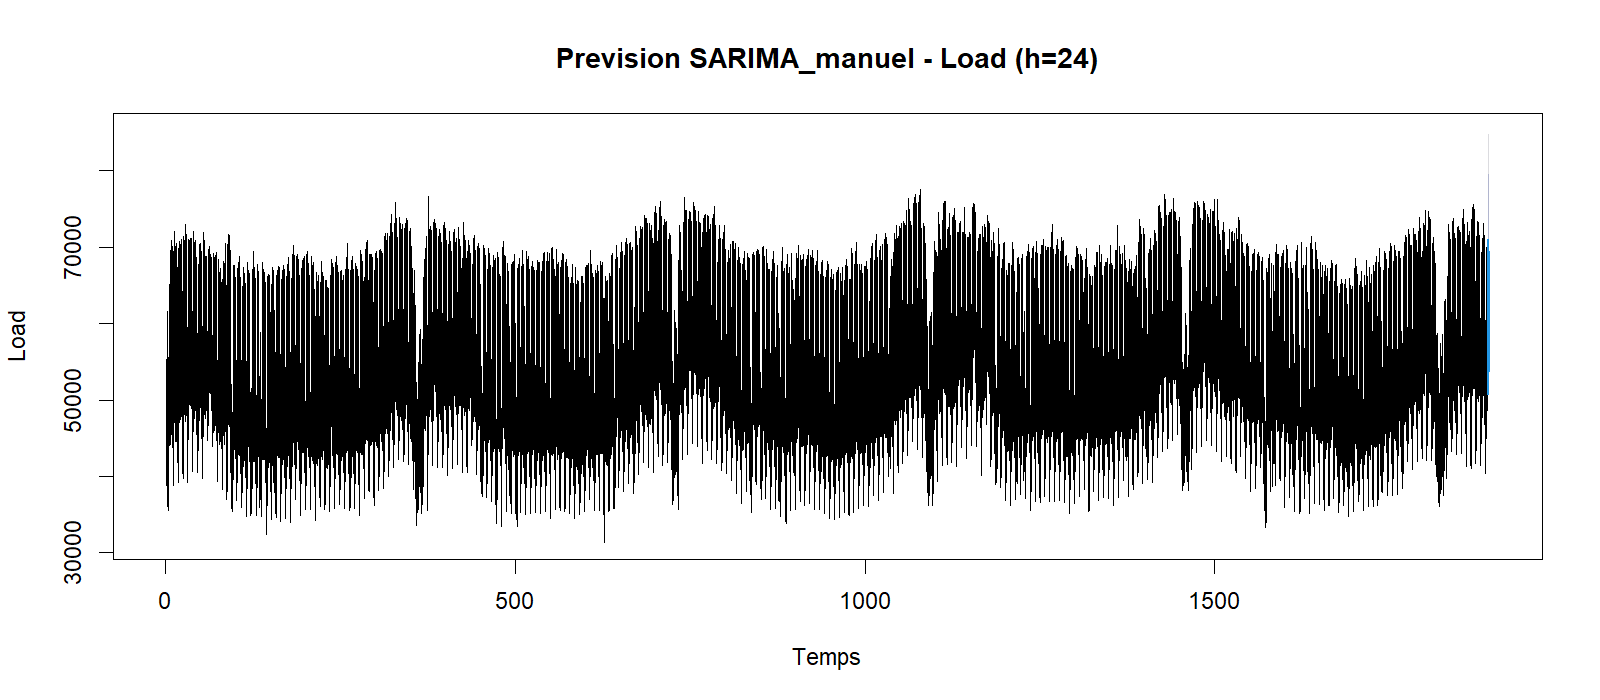
\includegraphics[width=0.9\textwidth]{R_prev_Load.png}
\caption{Prévision \texttt{Load} à \(h=24\) (modèle retenu, R).}
\label{fig:prev_r_load}
\end{figure}

\begin{figure}[H]
\centering
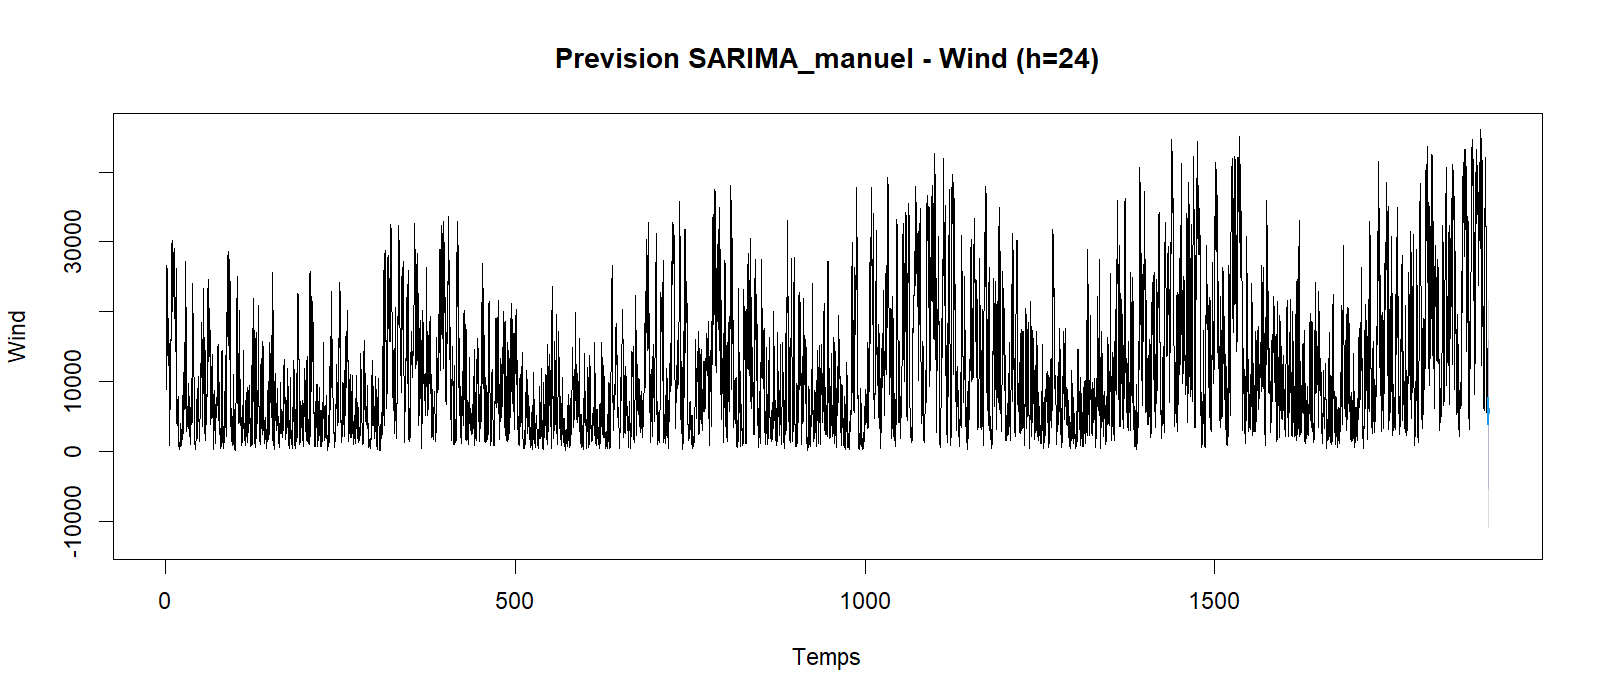
\includegraphics[width=0.9\textwidth]{R_prev_Wind.png}
\caption{Prévision \texttt{Wind} à \(h=24\) (R).}
\label{fig:prev_r_wind}
\end{figure}

\begin{figure}[H]
\centering
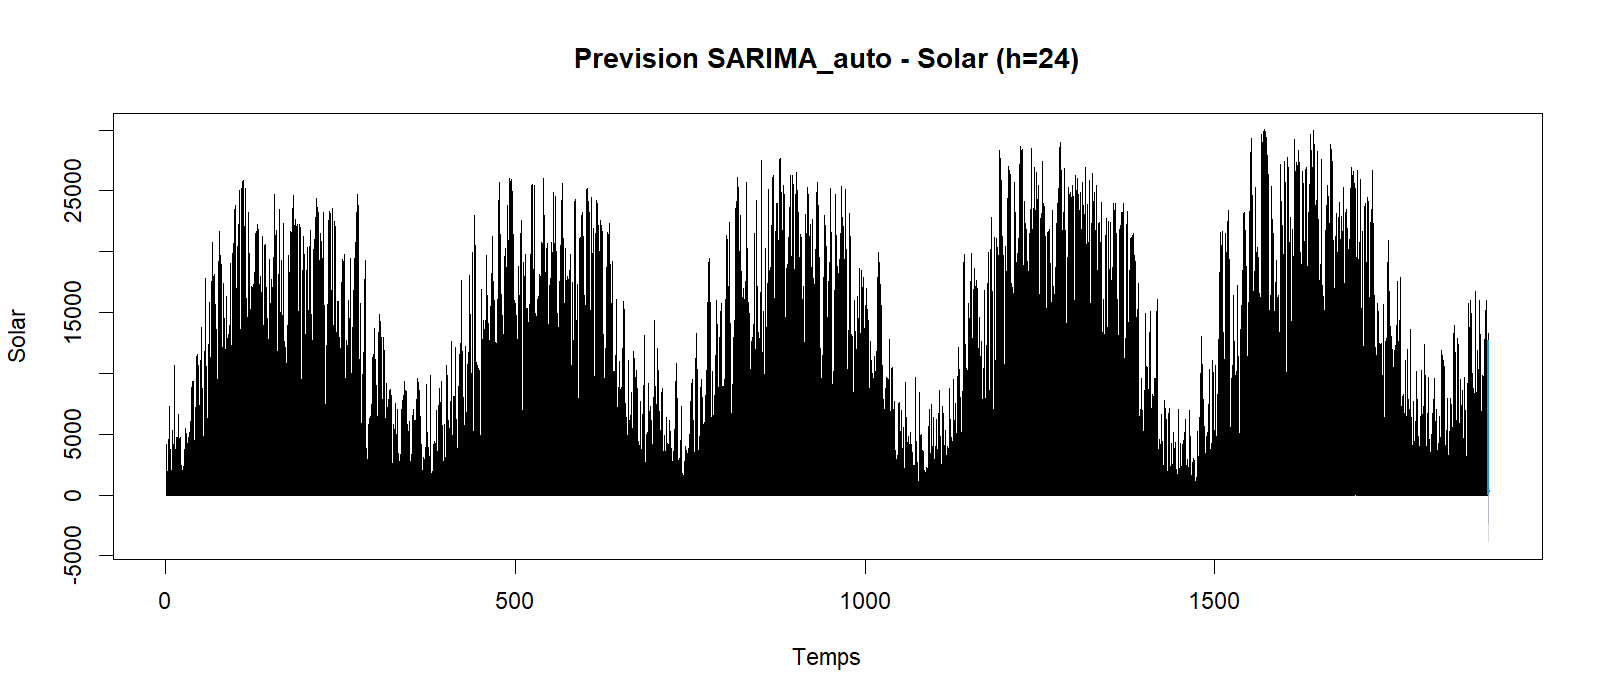
\includegraphics[width=0.9\textwidth]{R_prev_Solar.png}
\caption{Prévision \texttt{Solar} à \(h=24\) (R).}
\label{fig:prev_r_solar}
\end{figure}

\begin{figure}[H]
\centering
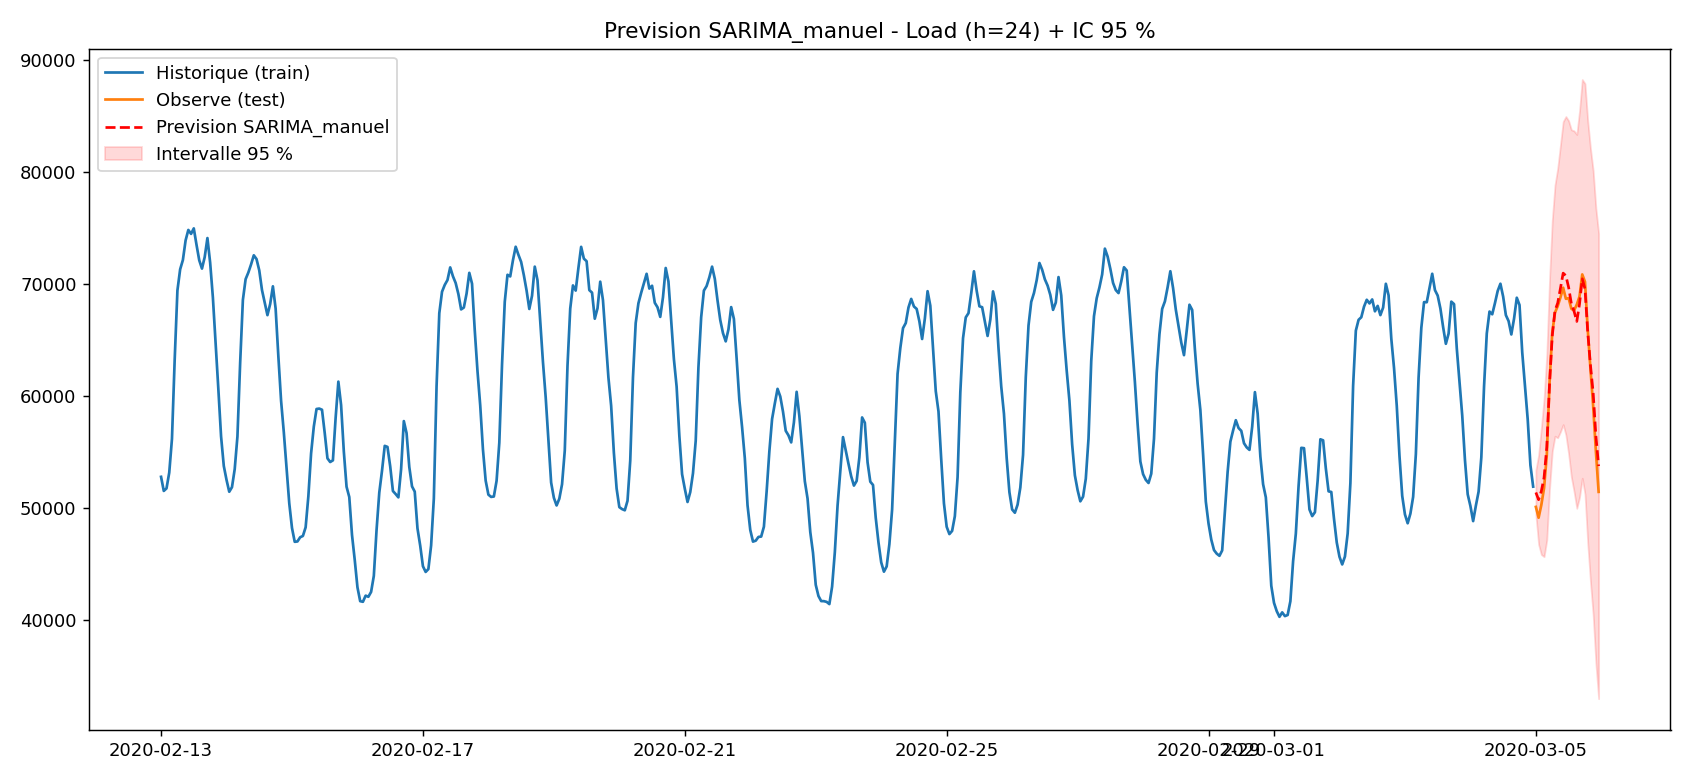
\includegraphics[width=0.9\textwidth]{py_prev_Load.png}
\caption{Prévision \texttt{Load} (Python) --- cohérente avec R.}
\label{fig:prev_py_load}
\end{figure}

\begin{figure}[H]
\centering
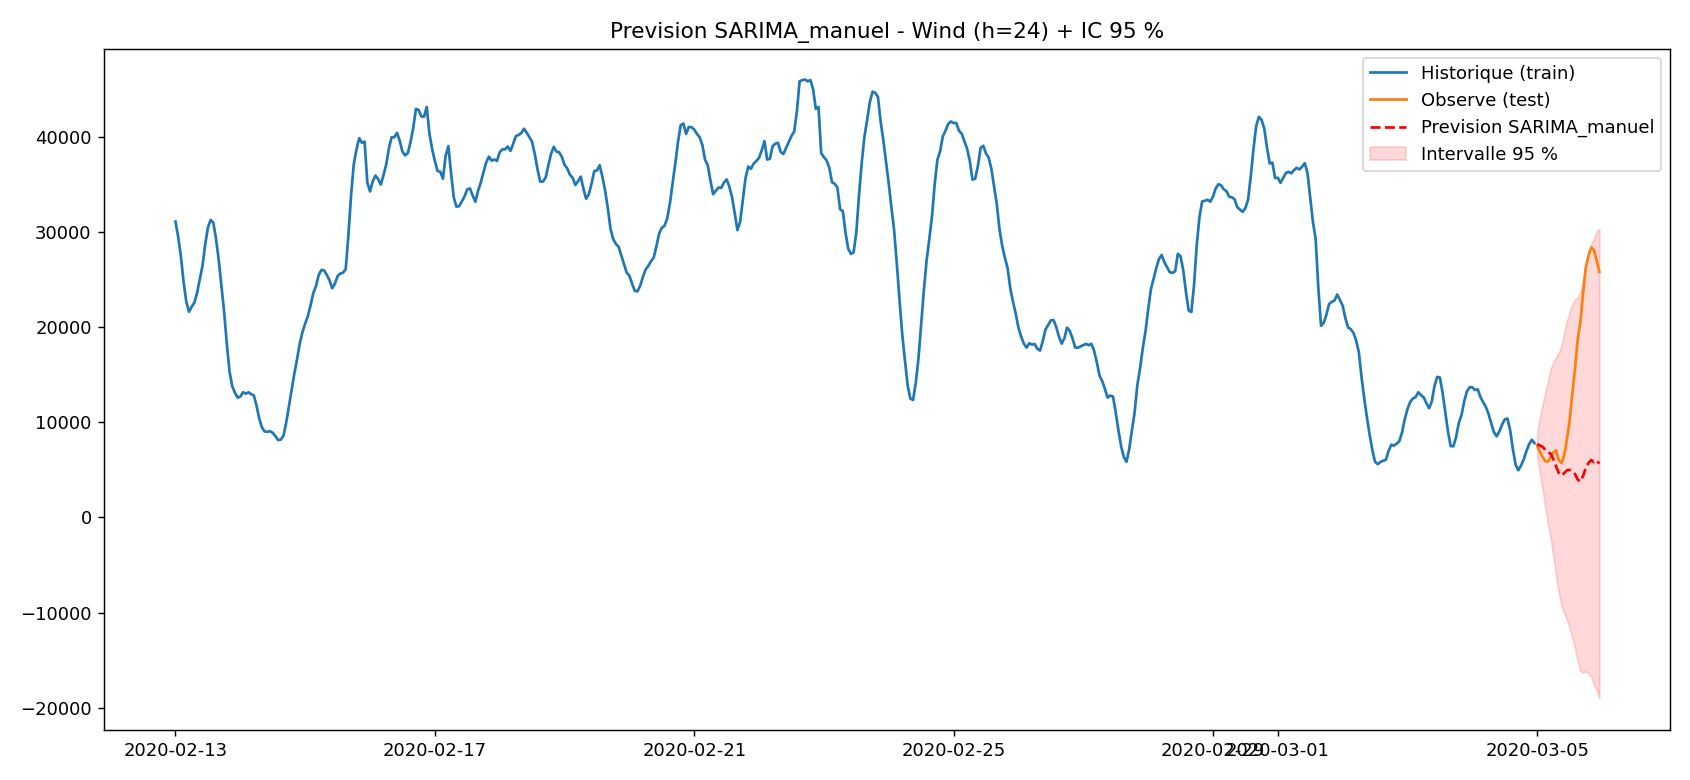
\includegraphics[width=0.9\textwidth]{py_prev_Wind.png}
\caption{Prévision \texttt{Wind} (Python).}
\label{fig:prev_py_wind}
\end{figure}

\begin{figure}[H]
\centering
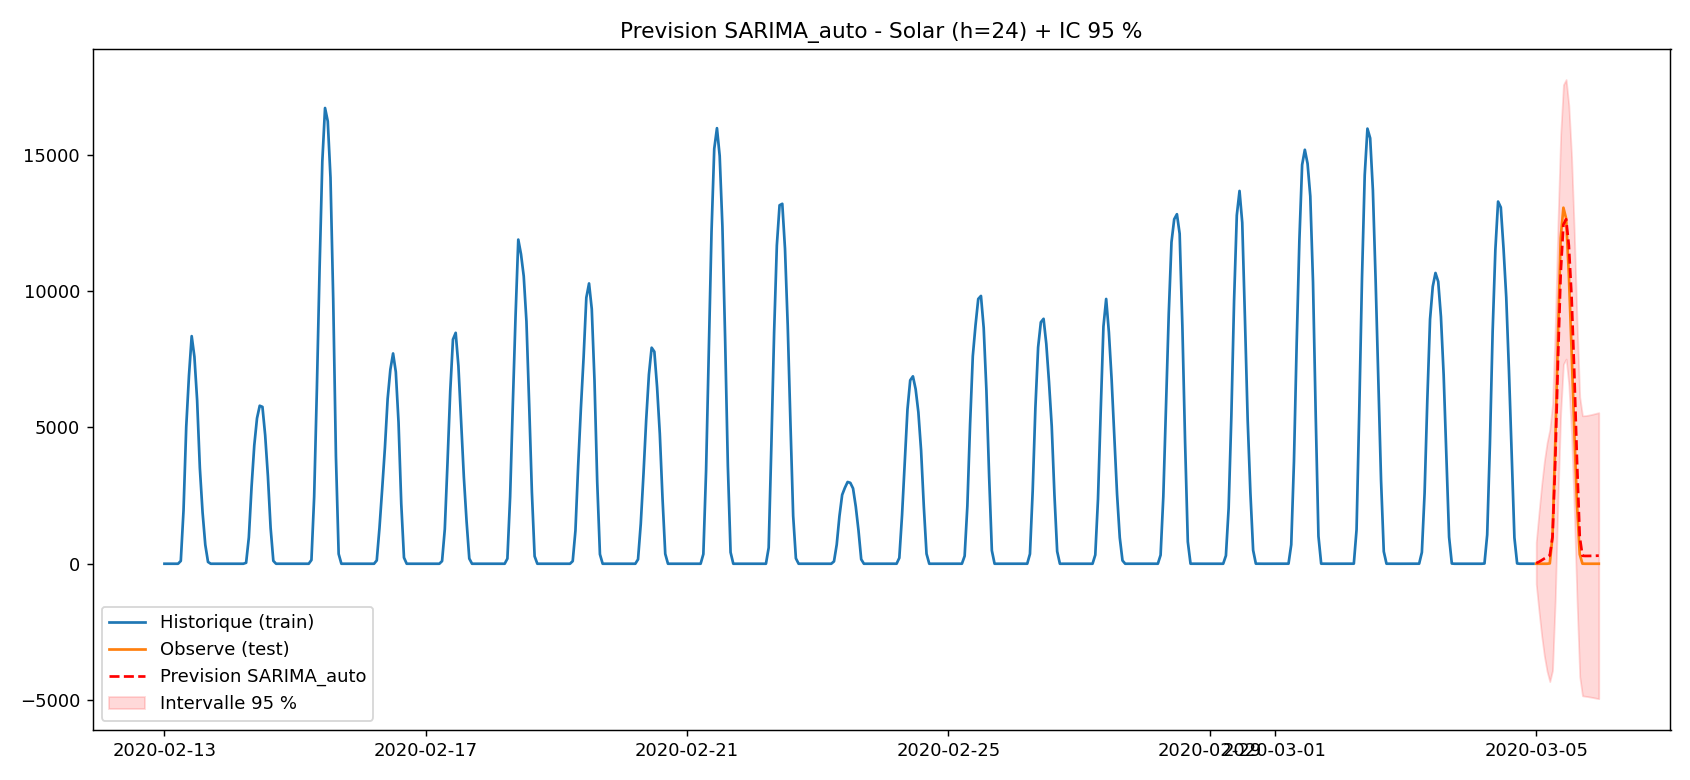
\includegraphics[width=0.9\textwidth]{py_prev_Solar.png}
\caption{Prévision \texttt{Solar} (Python).}
\label{fig:prev_py_solar}
\end{figure}

\begin{figure}[H]
\centering
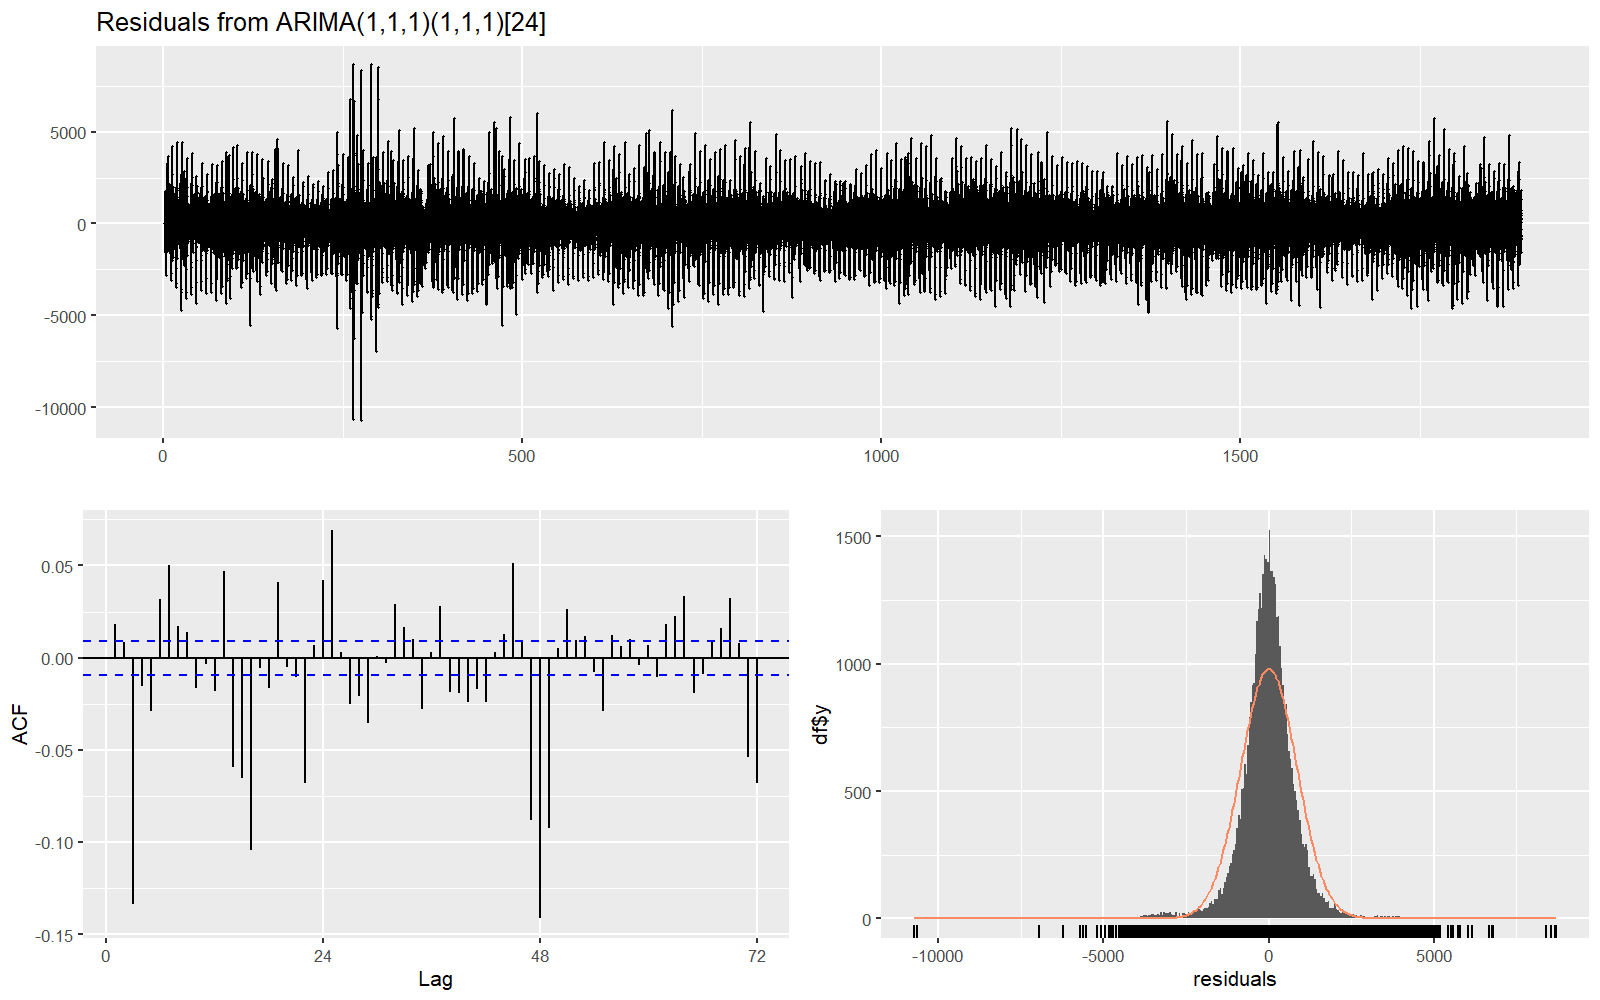
\includegraphics[width=0.9\textwidth]{R_resid_Load.png}
\caption{Diagnostic des résidus \texttt{Load} (R).}
\label{fig:resid_r_load}
\end{figure}

\begin{figure}[H]
\centering
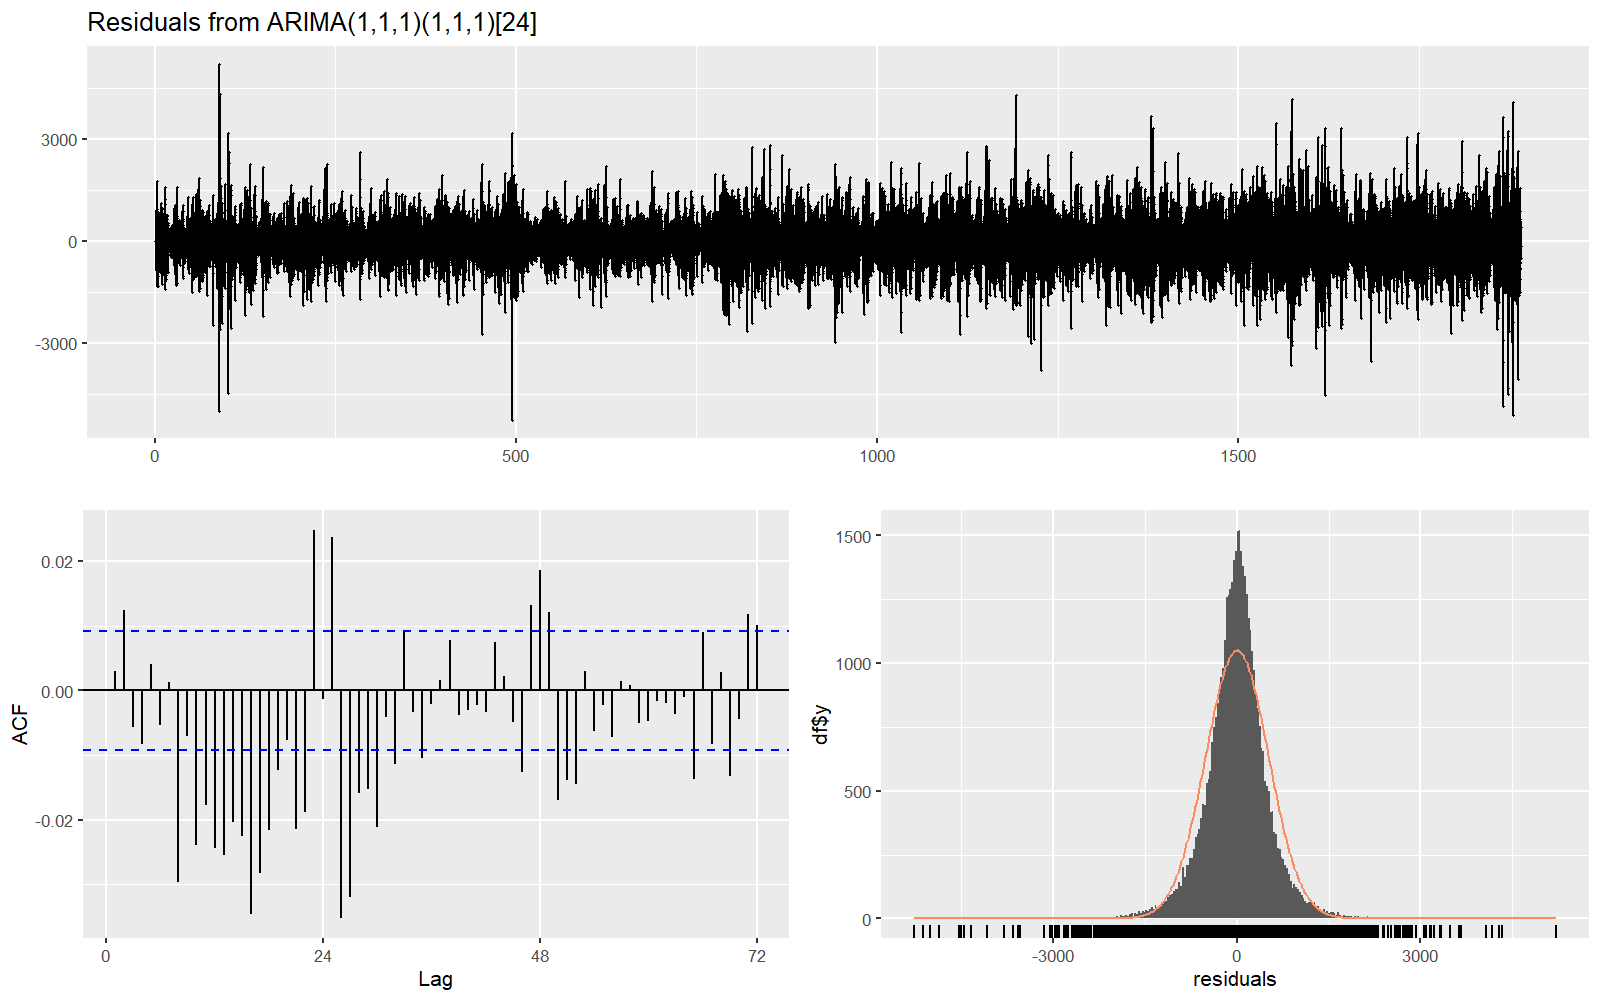
\includegraphics[width=0.9\textwidth]{R_resid_Wind.png}
\caption{Diagnostic des résidus \texttt{Wind} (R).}
\label{fig:resid_r_wind}
\end{figure}

\begin{figure}[H]
\centering
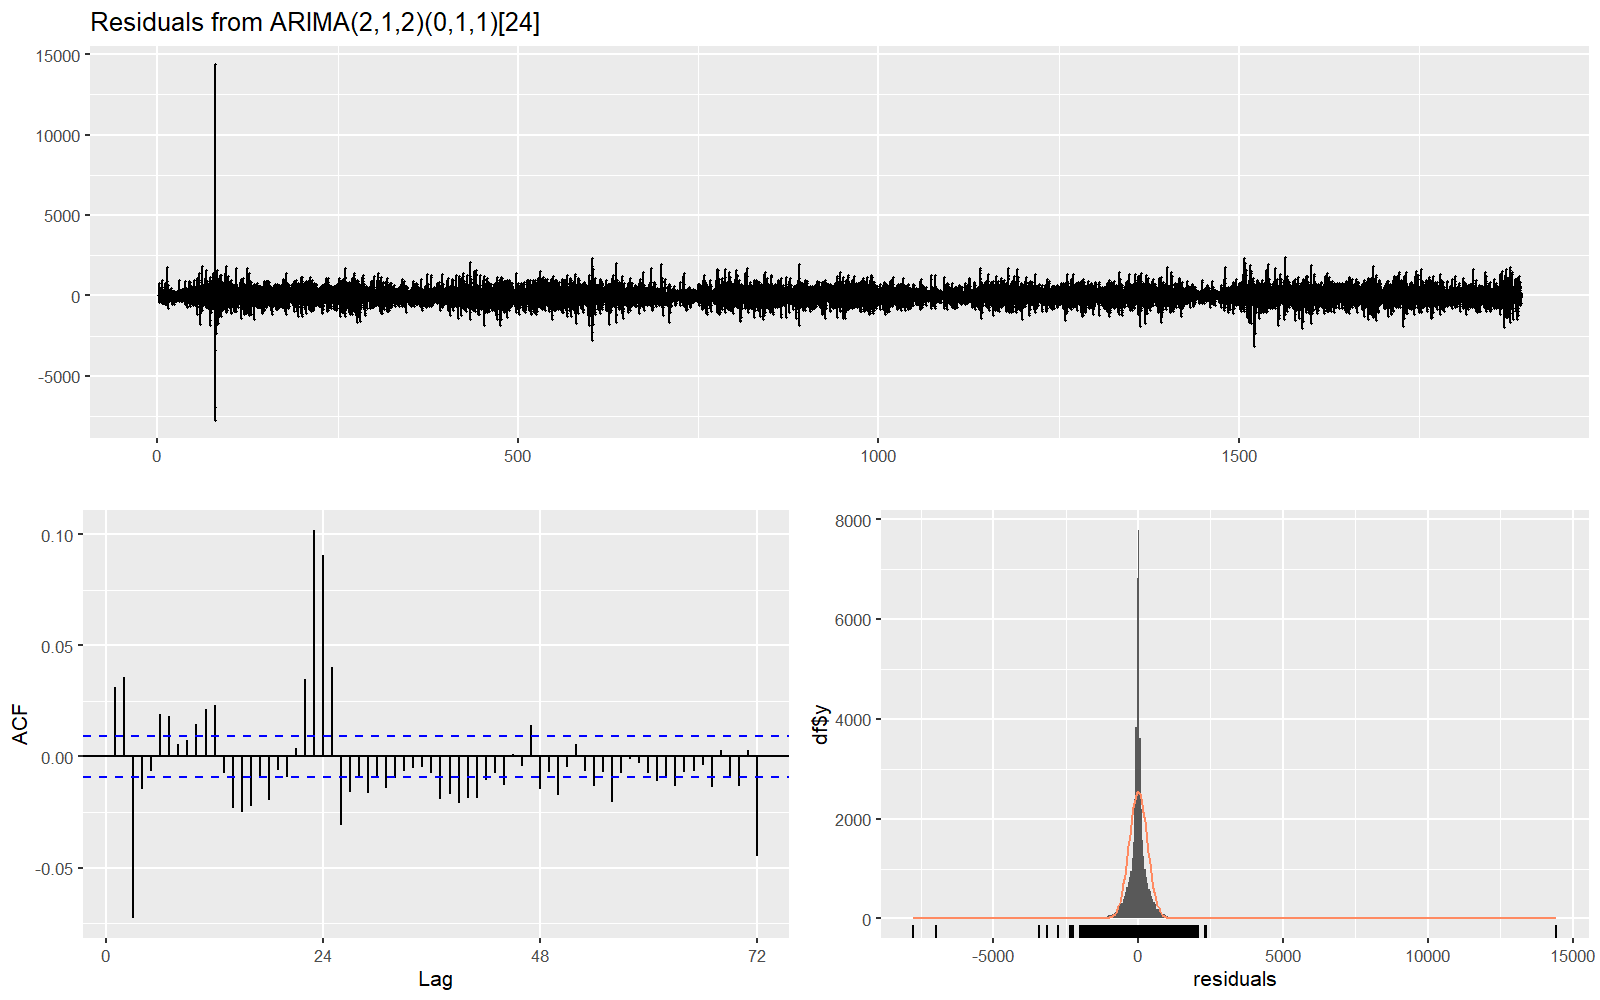
\includegraphics[width=0.9\textwidth]{R_resid_Solar.png}
\caption{Diagnostic des résidus \texttt{Solar} (R).}
\label{fig:resid_r_solar}
\end{figure}

\begin{figure}[H]
\centering
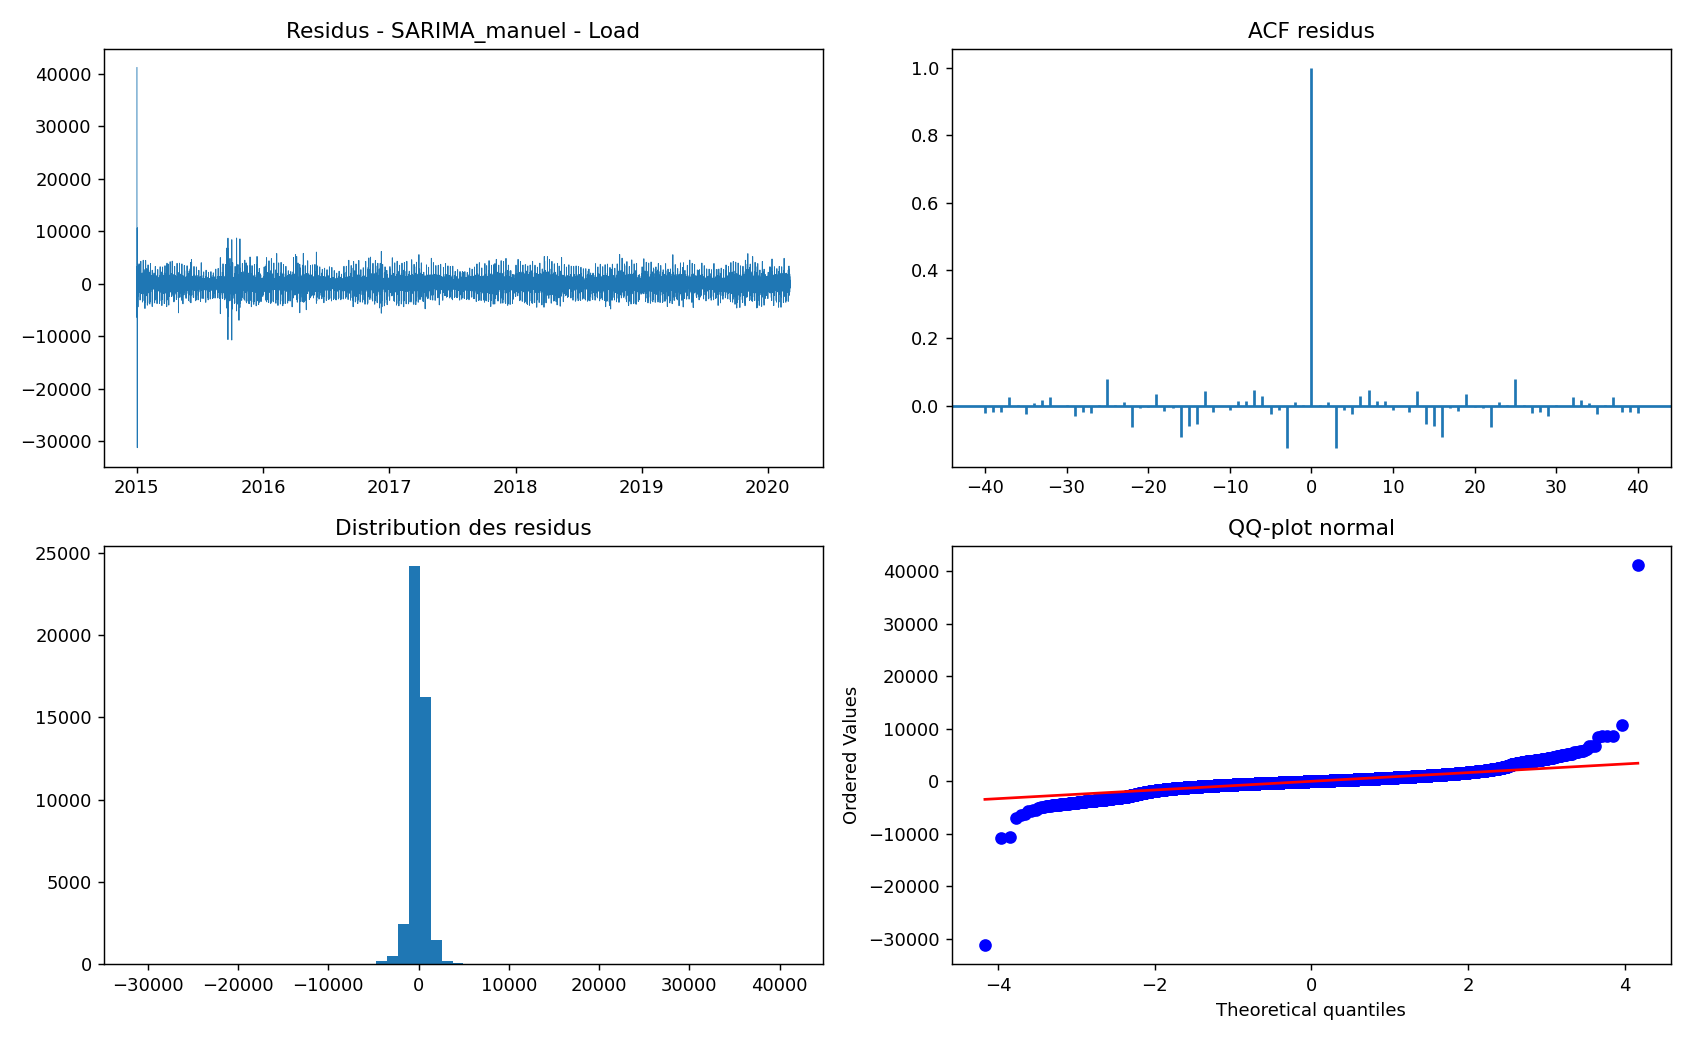
\includegraphics[width=0.9\textwidth]{py_resid_Load.png}
\caption{Diagnostic des résidus \texttt{Load} (Python).}
\label{fig:resid_py_load}
\end{figure}

\begin{figure}[H]
\centering
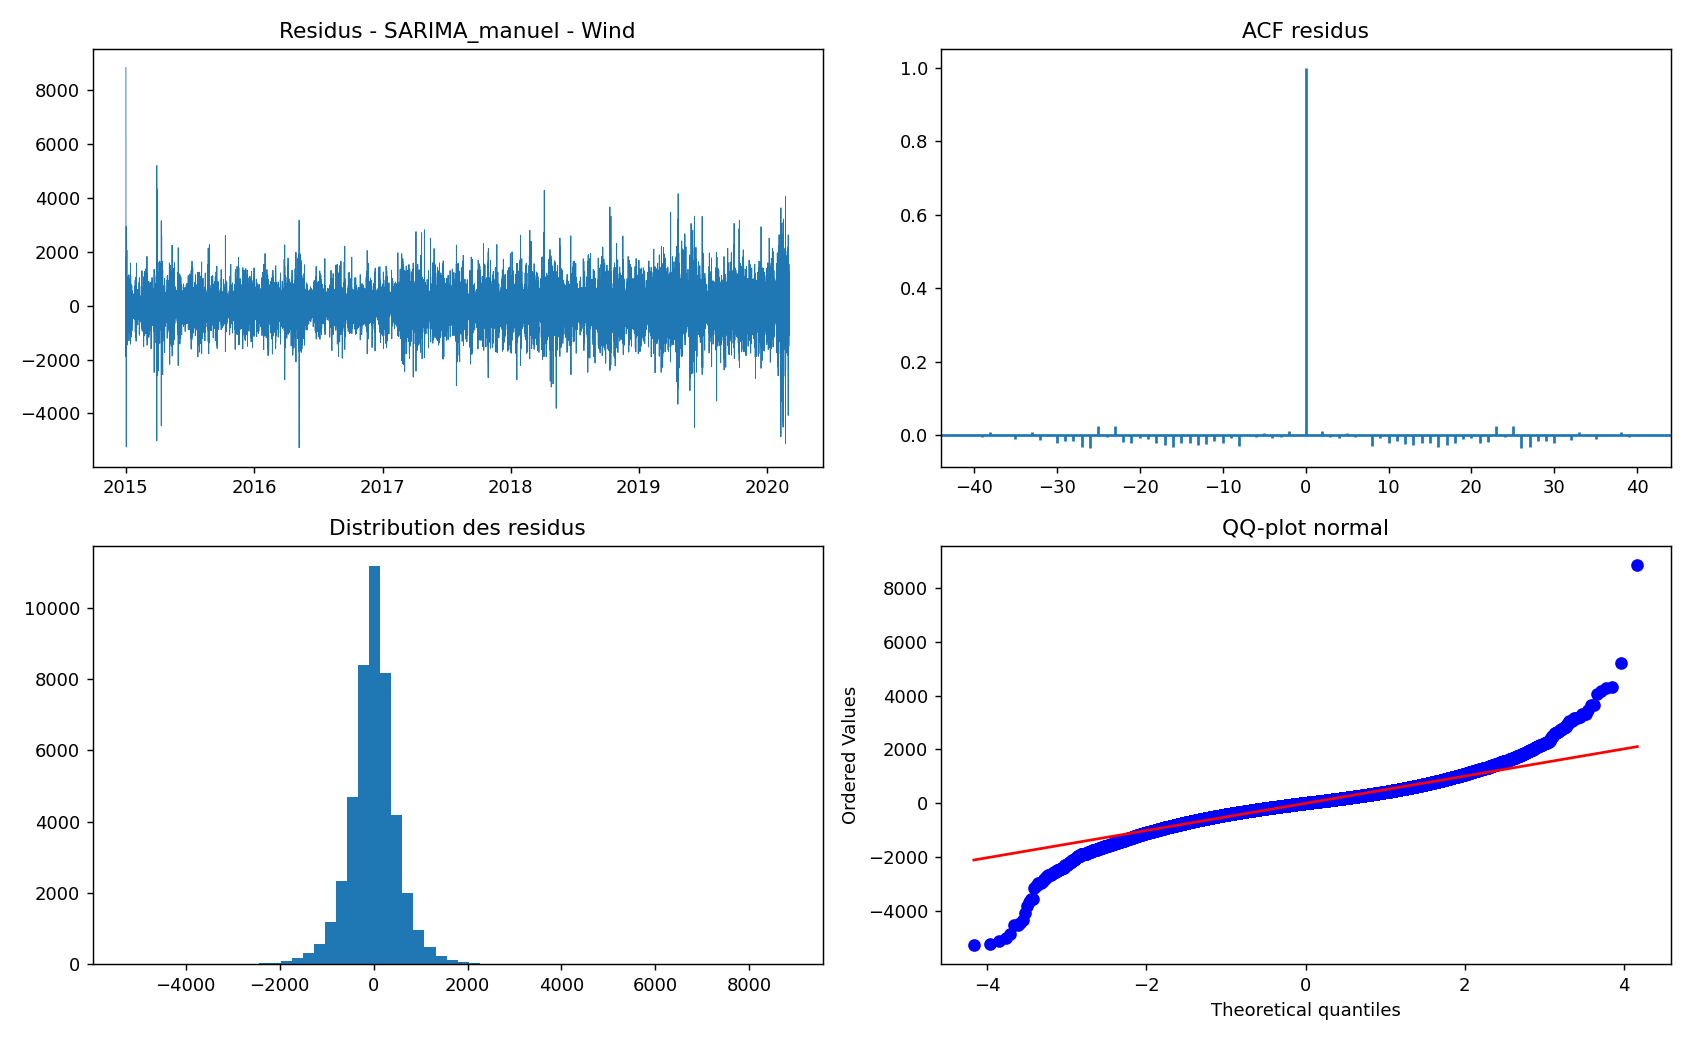
\includegraphics[width=0.9\textwidth]{py_resid_Wind.png}
\caption{Diagnostic des résidus \texttt{Wind} (Python).}
\label{fig:resid_py_wind}
\end{figure}

\begin{figure}[H]
\centering
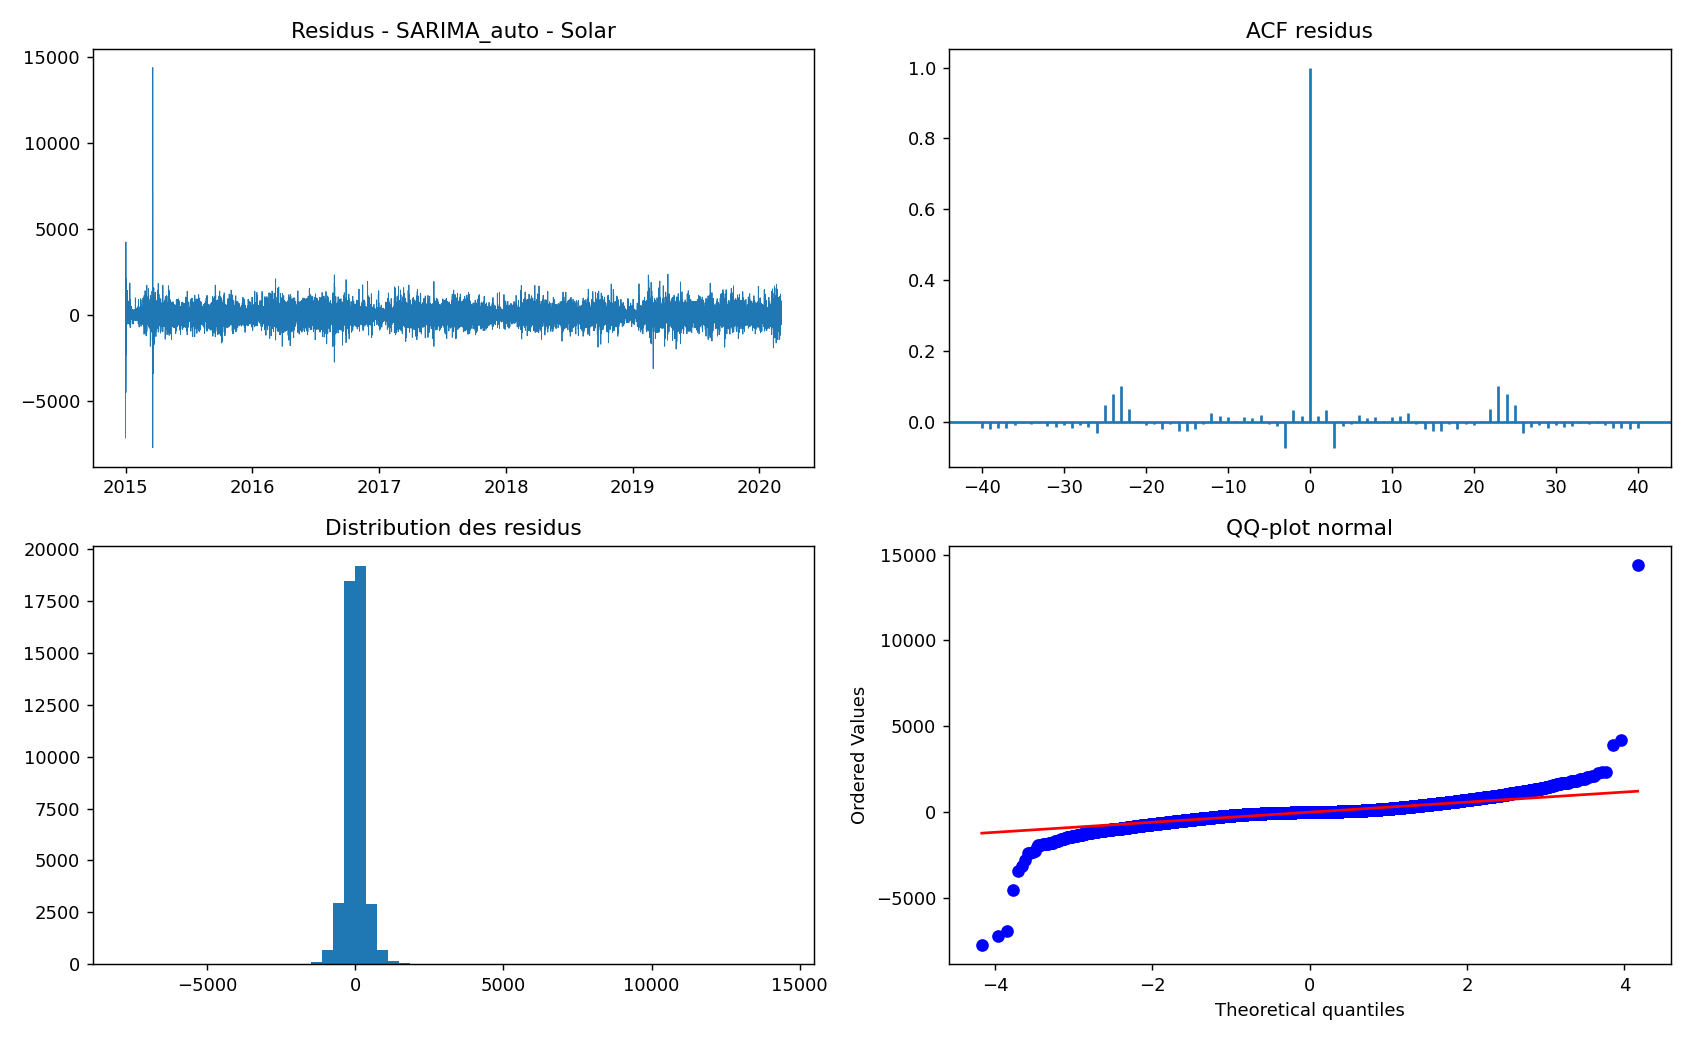
\includegraphics[width=0.9\textwidth]{py_resid_Solar.png}
\caption{Diagnostic des résidus \texttt{Solar} (Python).}
\label{fig:resid_py_solar}
\end{figure}

\FloatBarrier

\subsection{Liaisons dynamiques : VAR, Granger, Johansen, VECM}

\subsubsection{Sélection de l'ordre du VAR}
Le tableau~\ref{tab:var_order} (extrait de
\texttt{R\_var\_order.csv}) montre que le critère AIC atteint son minimum à
\(p=14\) (sur les moyennes journalières différenciées), retenu pour la suite.
Les critères HQ/SC suggèrent un ordre plus faible, mais l'AIC est privilégié
pour ne pas sous-paramétrer la dynamique. Python aboutit au même ordre
(\texttt{py\_var\_order.csv}).

\begin{table}[H]
\centering
\caption{Critères d'information pour la sélection de l'ordre du VAR (R).
Source : \texttt{R\_var\_order.csv}.}
\label{tab:var_order}
\small
\begin{tabular}{lrrrrrrrr}
\toprule
Critère & 10 & 11 & 12 & 13 & \textbf{14} & 15 \\
\midrule
AIC & 47{,}540 & 47{,}534 & 47{,}510 & 47{,}432 & \textbf{47{,}375} & 47{,}378 \\
HQ  & 47{,}641 & 47{,}645 & 47{,}631 & 47{,}563 & \textbf{47{,}516} & 47{,}528 \\
SC  & 47{,}815 & 47{,}835 & 47{,}838 & 47{,}787 & \textbf{47{,}757} & 47{,}786 \\
FPE & 4{,}43e20 & 4{,}40e20 & 4{,}30e20 & 3{,}98e20 & \textbf{3{,}76e20} & 3{,}77e20 \\
\bottomrule
\end{tabular}
\end{table}

\subsubsection{Causalité de Granger}
Le tableau~\ref{tab:granger} teste les six relations ordonnées. Seule
l'hypothèse \(\texttt{Wind} \to \texttt{Load}\) est rejetée (R : \(p=0{,}013\)
; Python : \(p=0{,}002\)), c'est-à-dire que la production éolienne
\textbf{cause} la consommation au sens de Granger. Aucune des autres
directions n'est significative.

\begin{table}[H]
\centering
\caption{Test de causalité de Granger (R et Python).
Sources : \texttt{R\_granger.csv}, \texttt{py\_granger.csv}.}
\label{tab:granger}
\small
\begin{tabular}{lrrl}
\toprule
Hypothèse & $p$ (R) & $p$ (py) & Conclusion \\
\midrule
\texttt{Wind} $\to$ \texttt{Load}  & \textbf{0{,}0126} & \textbf{0{,}0022} & Oui (rejet H0) \\
\texttt{Solar} $\to$ \texttt{Load} & 0{,}767 & 0{,}256 & Non \\
\texttt{Load} $\to$ \texttt{Wind}  & 0{,}244 & 0{,}157 & Non \\
\texttt{Solar} $\to$ \texttt{Wind} & 0{,}371 & 0{,}339 & Non \\
\texttt{Load} $\to$ \texttt{Solar}& 0{,}738 & 0{,}752 & Non \\
\texttt{Wind} $\to$ \texttt{Solar}& 0{,}099 & 0{,}058 & Non \\
\bottomrule
\end{tabular}
\end{table}

\subsubsection{Cointégration de Johansen et VECM}
Le test de trace de Johansen (tableau~\ref{tab:johansen}) conduit à
\textbf{\(r=2\)} relations de cointégration : au premier rang, la statistique
(\(155{,}32\)) dépasse largement la valeur critique (\(34{,}91\)) ; au second
rang (\(58{,}54\)) elle dépasse encore \(19{,}96\) ; au troisième rang
(\(8{,}67\)) elle passe sous \(9{,}24\). Ce résultat est \textbf{identique} en
R et en Python.

\begin{table}[H]
\centering
\caption{Test de trace de Johansen (valeurs critiques à 95\,\%).
Sources : \texttt{R\_johansen.csv}, \texttt{py\_johansen.csv}.}
\label{tab:johansen}
\small
\begin{tabular}{lrrrr}
\toprule
Rang testé & Stat. (R) & Stat. (py) & CV 95\,\% & Conclusion \\
\midrule
$r=0$ & 152{,}97 & 155{,}32 & 34{,}91 & Rejet $r=0$ \\
$r\leq 1$ & 57{,}83 & 58{,}54 & 19{,}96 & Rejet $r\leq 1$ \\
$r\leq 2$ & 8{,}66 & 8{,}67 & 9{,}24 & Non rejeté \\
\bottomrule
\end{tabular}
\end{table}

Le VECM estimé (tableaux~\ref{tab:vecm} et~\ref{tab:vecm_alpha}) fournit des
vecteurs de cointégration \(\beta\) normalisés très proches en R et Python
(\texttt{Solar} : \(\approx 0{,}91\) et \(\approx 1{,}22\) sur les deux
relations) et des vitesses d'ajustement \(\alpha\) cohérentes : la charge et
l'éolien présentent une force de rappel significative
(\(\alpha \approx -0{,}24\) pour \texttt{Load} dans l'équation 1 et
\texttt{Wind} dans l'équation 2), tandis que le solaire s'ajuste très peu.

\begin{table}[H]
\centering
\caption{Vecteurs de cointégration normalisés $\beta$ du VECM
(\(r=2\)). Sources : \texttt{R\_vecm.csv}, \texttt{py\_vecm.csv}.}
\label{tab:vecm}
\small
\begin{tabular}{lrr}
\toprule
Variable (lag 1) & ECT\_1 & ECT\_2 \\
\midrule
\texttt{Load}  & 1{,}0000 & 0{,}0000 \\
\texttt{Wind}  & 0{,}0000 & 1{,}0000 \\
\texttt{Solar} & 0{,}9084 (py 0{,}9148) & 1{,}2126 (py 1{,}2222) \\
Constante      & $-59\,819$ (py $-59\,848$) & $-16\,705$ (py $-16\,780$) \\
\bottomrule
\end{tabular}
\end{table}

\begin{table}[H]
\centering
\caption{Vitesses d'ajustement $\alpha$ du VECM.
Sources : \texttt{R\_vecm\_alpha.csv}, \texttt{py\_vecm\_alpha.csv}.}
\label{tab:vecm_alpha}
\small
\begin{tabular}{lrrr}
\toprule
Équation & $\Delta$\texttt{Load} & $\Delta$\texttt{Wind} & $\Delta$\texttt{Solar} \\
\midrule
ECT\_1 & $-0{,}2379$ & $0{,}1196$ & $0{,}0030$ \\
ECT\_2 & $0{,}0161$ & $-0{,}2396$ & $0{,}0063$ \\
\bottomrule
\end{tabular}
\end{table}

\subsubsection{Diagnostics du VAR}
Le tableau~\ref{tab:var_diag} indique le rejet des trois tests : le VAR
journalier laisse une autocorrélation, une non-normalité et surtout un effet
\textbf{ARCH multivarié}, ce qui confirme une nouvelle fois le besoin d'une
modélisation explicite de la volatilité.

\begin{table}[H]
\centering
\caption{Diagnostics multivariés du VAR. Sources :
\texttt{R\_var\_diagnostics.csv}, \texttt{py\_var\_diagnostics.csv}.}
\label{tab:var_diag}
\small
\begin{tabular}{lrr}
\toprule
Test & $p$ (R) & $p$ (py) \\
\midrule
Portmanteau (autocorrélation) & $<0{,}001$ & $5{,}0\text{e-}40$ \\
Normalité multivariée (JB) & $<0{,}001$ & $<0{,}001$ \\
ARCH multivarié (Load) & $<0{,}001$ & $1{,}1\text{e-}24$ \\
ARCH multivarié (Wind) & --- & $2{,}6\text{e-}16$ \\
ARCH multivarié (Solar) & --- & $4{,}6\text{e-}15$ \\
\bottomrule
\end{tabular}
\end{table}

\subsubsection{Réponse impulsionnelle et décomposition de la variance}
Les figures~\ref{fig:irf_r} et~\ref{fig:fevd_r} (et leurs homologues Python
\ref{fig:irf_py} et~\ref{fig:fevd_py}) synthétisent les dynamiques. La
décomposition de variance à \(28\) jours (tableau~\ref{tab:fevd_summary})
montre que chaque série est essentiellement expliquée par elle-même
(\(92\) à \(97\,\%\)), avec une contribution de \texttt{Wind} à \texttt{Load}
d'environ \(2{,}2\,\%\) et de \texttt{Solar} à \texttt{Load} d'environ
\(4{,}1\,\%\) --- cohérent avec la causalité de Granger détectée.

\begin{figure}[H]
\centering
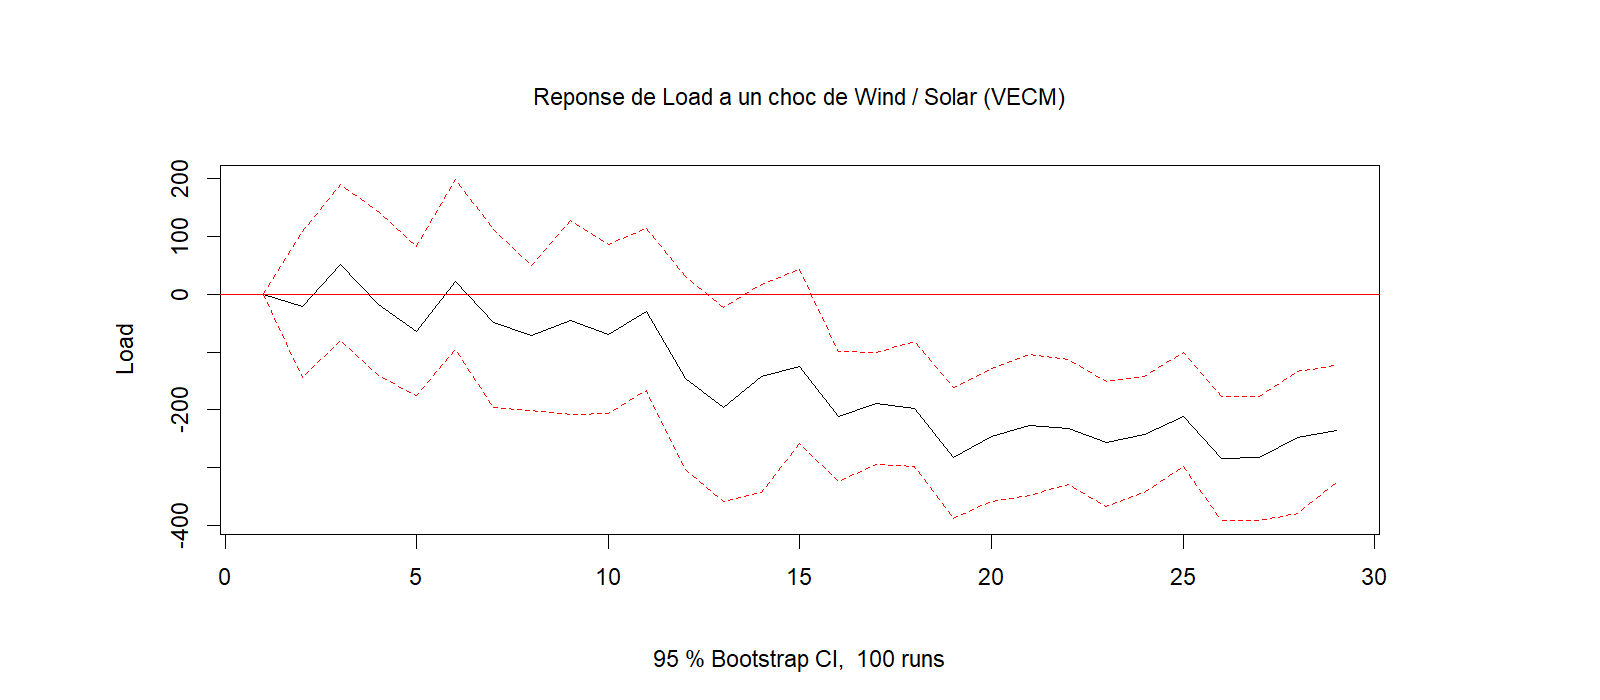
\includegraphics[width=0.9\textwidth]{R_var_irf_load.png}
\caption{Réponse de \texttt{Load} à un choc de \texttt{Wind}/\texttt{Solar} (R, 28 jours).}
\label{fig:irf_r}
\end{figure}

\begin{figure}[H]
\centering
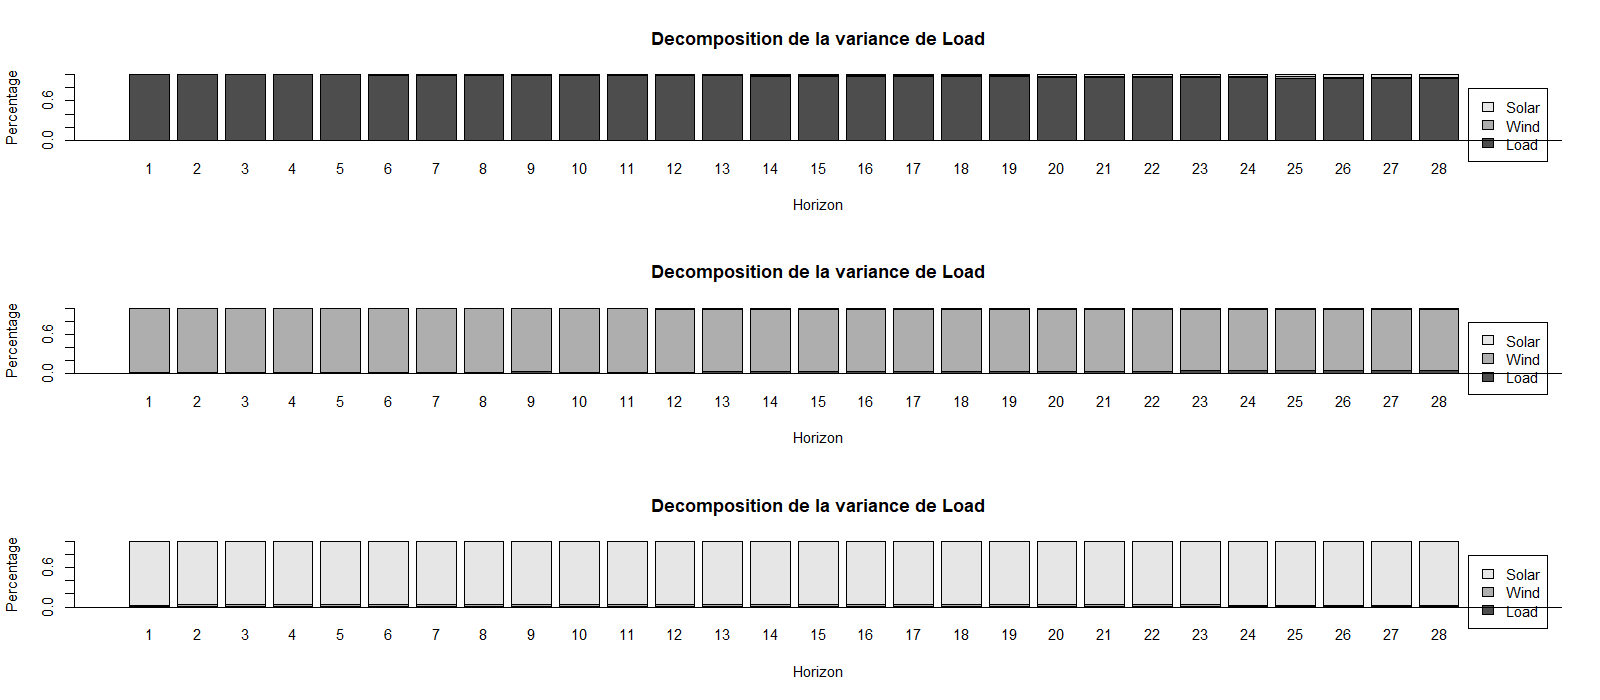
\includegraphics[width=0.9\textwidth]{R_var_fevd_load.png}
\caption{Décomposition de la variance de \texttt{Load} (R).}
\label{fig:fevd_r}
\end{figure}

\begin{figure}[H]
\centering
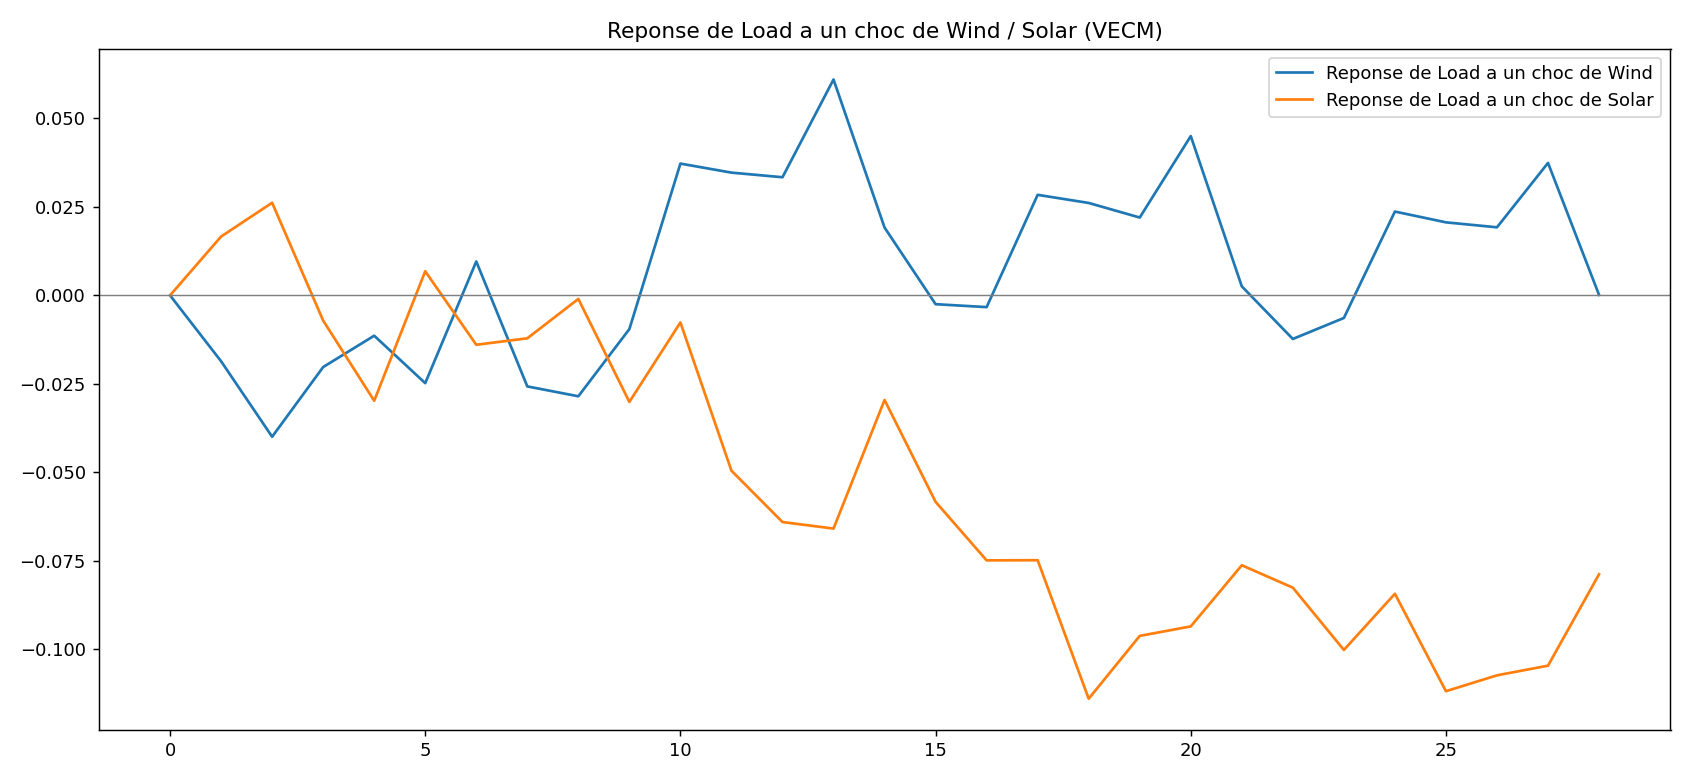
\includegraphics[width=0.9\textwidth]{py_var_irf_load.png}
\caption{Réponse de \texttt{Load} à un choc (Python).}
\label{fig:irf_py}
\end{figure}

\begin{figure}[H]
\centering
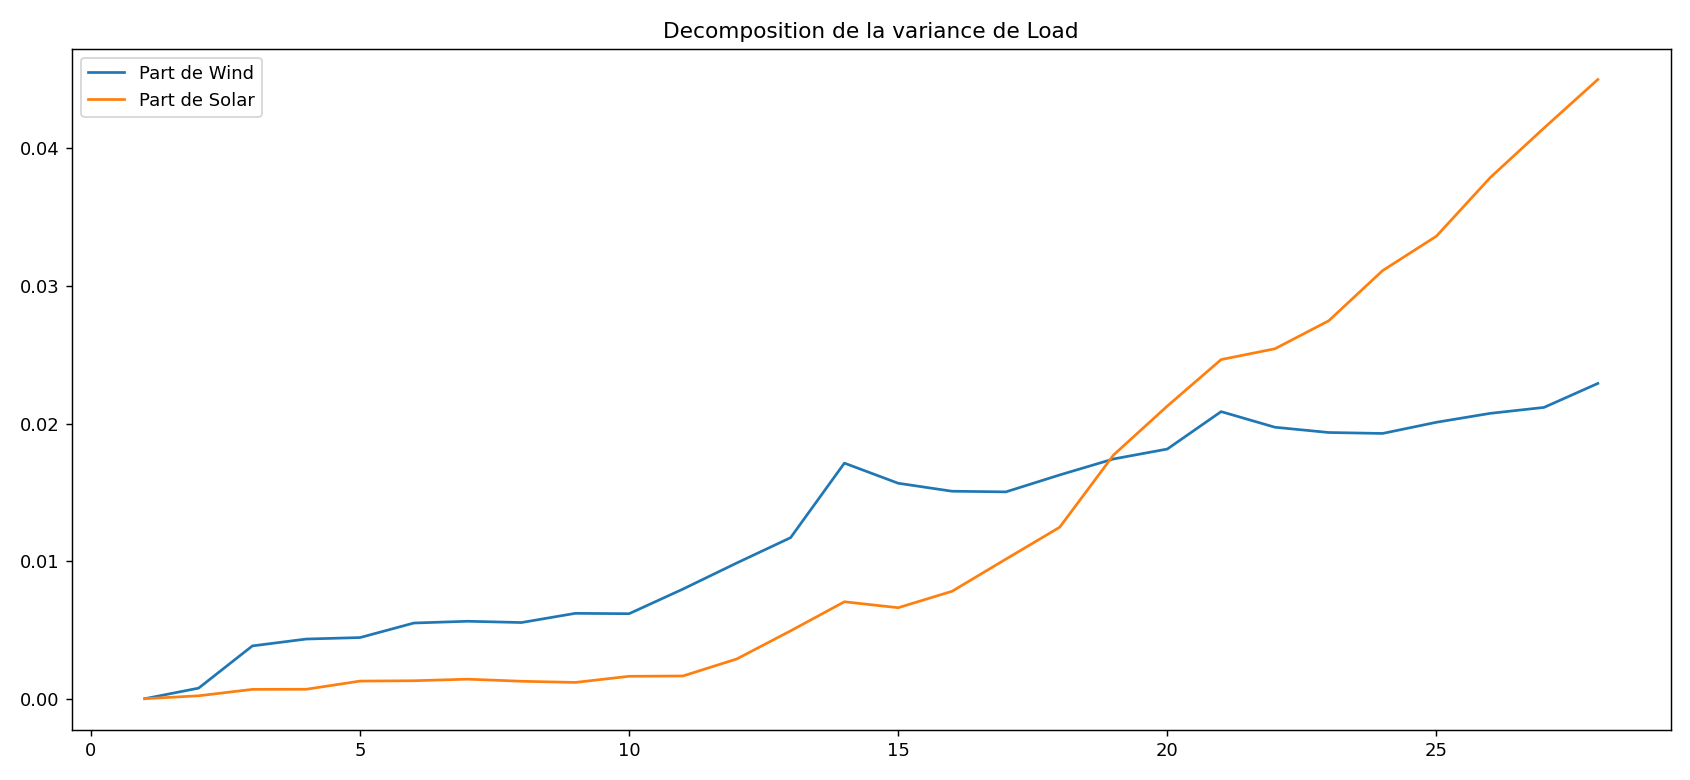
\includegraphics[width=0.9\textwidth]{py_var_fevd_load.png}
\caption{Décomposition de la variance de \texttt{Load} (Python).}
\label{fig:fevd_py}
\end{figure}

\begin{table}[H]
\centering
\caption{Décomposition de la variance au jour 28 (R).
Source : \texttt{R\_var\_fevd.csv}.}
\label{tab:fevd_summary}
\small
\begin{tabular}{lrrr}
\toprule
Variable expliquée & Part \texttt{Load} & Part \texttt{Wind} & Part \texttt{Solar} \\
\midrule
\texttt{Load}  & 0{,}9368 & 0{,}0219 & 0{,}0413 \\
\texttt{Wind}  & 0{,}0459 & 0{,}9243 & 0{,}0298 \\
\texttt{Solar} & 0{,}0080 & 0{,}0213 & 0{,}9708 \\
\bottomrule
\end{tabular}
\end{table}

\FloatBarrier

\subsection{Modélisation de la volatilité : ARCH / GARCH}
\label{sec:garch}

\subsubsection{Persistance de la volatilité}
Le tableau~\ref{tab:garch_pers_r} (R) et le tableau~\ref{tab:garch_pers_py}
(Python) résument la persistance. Pour \texttt{Wind}, les trois spécifications
sont covariation-stationnaires avec une persistance très élevée
(\(\approx 0{,}99\)), soit une demi-vie de \(68\) (GARCH(1,1)) à \(675\)
(EGARCH) jours. Pour \texttt{Load}, GARCH(1,1) est proche de la frontière
(persistance \(\approx 0{,}998\) en R). Pour \texttt{Solar}, GARCH(1,1) et
GARCH(2,1) sont non stationnaires (persistance \(\geq 1\)), seul
l'EGARCH(1,1) reste stable (\(\approx 0{,}99\)).

\begin{table}[H]
\centering
\caption{Persistance de la volatilité (R).
Source : \texttt{R\_garch\_persistence.csv}.}
\label{tab:garch_pers_r}
\small
\begin{tabular}{llrrl}
\toprule
Variable & Modèle & Persistance & Demi-vie (j) & Cov. stationnaire \\
\midrule
\texttt{Load}  & GARCH(1,1)  & 0{,}9981 & 366{,}8 & Oui \\
\texttt{Load}  & GARCH(2,1)  & 0{,}4540 & 0{,}9 & Oui \\
\texttt{Load}  & EGARCH(1,1) & 0{,}6312 & 1{,}5 & Oui \\
\texttt{Wind}  & GARCH(1,1)  & 0{,}9899 & 68{,}5 & Oui \\
\texttt{Wind}  & GARCH(2,1)  & 0{,}9875 & 55{,}3 & Oui \\
\texttt{Wind}  & EGARCH(1,1) & 0{,}9990 & 675{,}2 & Oui \\
\texttt{Solar} & GARCH(1,1)  & 1{,}0050 & NA & Non \\
\texttt{Solar} & GARCH(2,1)  & 1{,}0051 & NA & Non \\
\texttt{Solar} & EGARCH(1,1) & 0{,}9936 & 108{,}3 & Oui \\
\bottomrule
\end{tabular}
\end{table}

\begin{table}[H]
\centering
\caption{Persistance de la volatilité (Python).
Source : \texttt{py\_garch\_persistence.csv}.}
\label{tab:garch_pers_py}
\small
\begin{tabular}{llrrl}
\toprule
Variable & Modèle & Persistance & Demi-vie (j) & Convergence \\
\midrule
\texttt{Load}  & GARCH(1,1)  & --- & --- & Non \\
\texttt{Load}  & GARCH(2,1)  & 0{,}8222 & 3{,}5 & Oui \\
\texttt{Load}  & EGARCH(1,1) & --- & --- & Non \\
\texttt{Wind}  & GARCH(1,1)  & 0{,}9905 & 72{,}7 & Oui \\
\texttt{Wind}  & GARCH(2,1)  & 0{,}9892 & 63{,}6 & Oui \\
\texttt{Wind}  & EGARCH(1,1) & 0{,}9861 & 49{,}3 & Oui \\
\texttt{Solar} & GARCH(1,1)  & 1{,}0000 & --- & Non \\
\texttt{Solar} & GARCH(2,1)  & 1{,}0000 & --- & Non \\
\texttt{Solar} & EGARCH(1,1) & 0{,}9894 & 65{,}0 & Oui \\
\bottomrule
\end{tabular}
\end{table}

\subsubsection{Coefficients estimés}
Le tableau~\ref{tab:garch_coef_py} détaille les coefficients estimés en
Python (avec AIC/BIC et paramètre de queue lourde \(\nu_t\)). On note pour
\texttt{Wind} un \(\beta_1 \approx 0{,}935\) (persistance de la volatilité) et
pour \texttt{Solar} un \(\nu_t \approx 8{,}7\), confirmant des queues plus
épaisses que la normale.

\begin{table}[H]
\centering
\caption{Coefficients GARCH estimés (Python).
Source : \texttt{py\_garch\_coefficients.csv}.}
\label{tab:garch_coef_py}
\small
\begin{tabular}{llrrrrrr}
\toprule
Variable & Modèle & $\mu$ & $\omega$ & $\alpha_1$ & $\beta_1$ & Pers. & $\nu_t$ \\
\midrule
\texttt{Load}  & GARCH(2,1)  & $-0{,}186$ & 1{,}296 & 0{,}0013 & 0{,}8209 & 0{,}822 & 2{,}05 \\
\texttt{Wind}  & GARCH(1,1)  & $-0{,}004$ & 0{,}0113 & 0{,}0553 & 0{,}9352 & 0{,}991 & 7{,}35 \\
\texttt{Wind}  & EGARCH(1,1) & $-0{,}005$ & 0{,}0039 & 0{,}1205 & 0{,}9861 & 0{,}986 & 7{,}33 \\
\texttt{Solar} & GARCH(1,1)  & $-0{,}001$ & 0{,}0042 & 0{,}0890 & 0{,}9110 & 1{,}000 & 8{,}72 \\
\texttt{Solar} & EGARCH(1,1) & $0{,}000$  & 0{,}0056 & 0{,}1942 & 0{,}9894 & 0{,}989 & 8{,}09 \\
\bottomrule
\end{tabular}
\end{table}

\subsubsection{Diagnostics GARCH et volatilité conditionnelle}
Le tableau~\ref{tab:garch_diag} montre que les résidus standardisés du
GARCH(1,1) ne sont plus autocorrélés (Ljung--Box des résidus) et que, pour
\texttt{Solar}, les résidus au carré ne présentent plus d'effet ARCH (GARCH
capture bien la volatilité), tandis que la non-normalité persiste (attendu avec
une loi de Student).

\begin{table}[H]
\centering
\caption{Diagnostics du GARCH(1,1). Sources :
\texttt{R\_garch\_diagnostics.csv}, \texttt{py\_garch\_diagnostics.csv}.}
\label{tab:garch_diag}
\small
\begin{tabular}{llrrr}
\toprule
Impl. & Variable & LB résidus $p$ & LB résidus$^2$ $p$ & JB $p$ \\
\midrule
R  & \texttt{Load}  & 0{,}000 & 0{,}000 & 0{,}000 \\
R  & \texttt{Wind}  & 0{,}000 & 0{,}010 & 0{,}000 \\
R  & \texttt{Solar} & 0{,}000 & 0{,}780 & $3{,}9\text{e-}11$ \\
py & \texttt{Load}  & 0{,}000 & 0{,}000 & $1{,}2\text{e-}86$ \\
py & \texttt{Wind}  & $8{,}2\text{e-}25$ & 0{,}015 & $3{,}7\text{e-}21$ \\
py & \texttt{Solar} & $8{,}1\text{e-}26$ & 0{,}850 & $3{,}7\text{e-}11$ \\
\bottomrule
\end{tabular}
\end{table}

Les figures~\ref{fig:garch_r_load}--\ref{fig:garch_r_solar} (R) et
\ref{fig:garch_py_load}--\ref{fig:garch_py_solar} (Python) représentent la
volatilité conditionnelle \(\sigma_t\) estimée et les épisodes de forte
volatilité.

\begin{figure}[H]
\centering
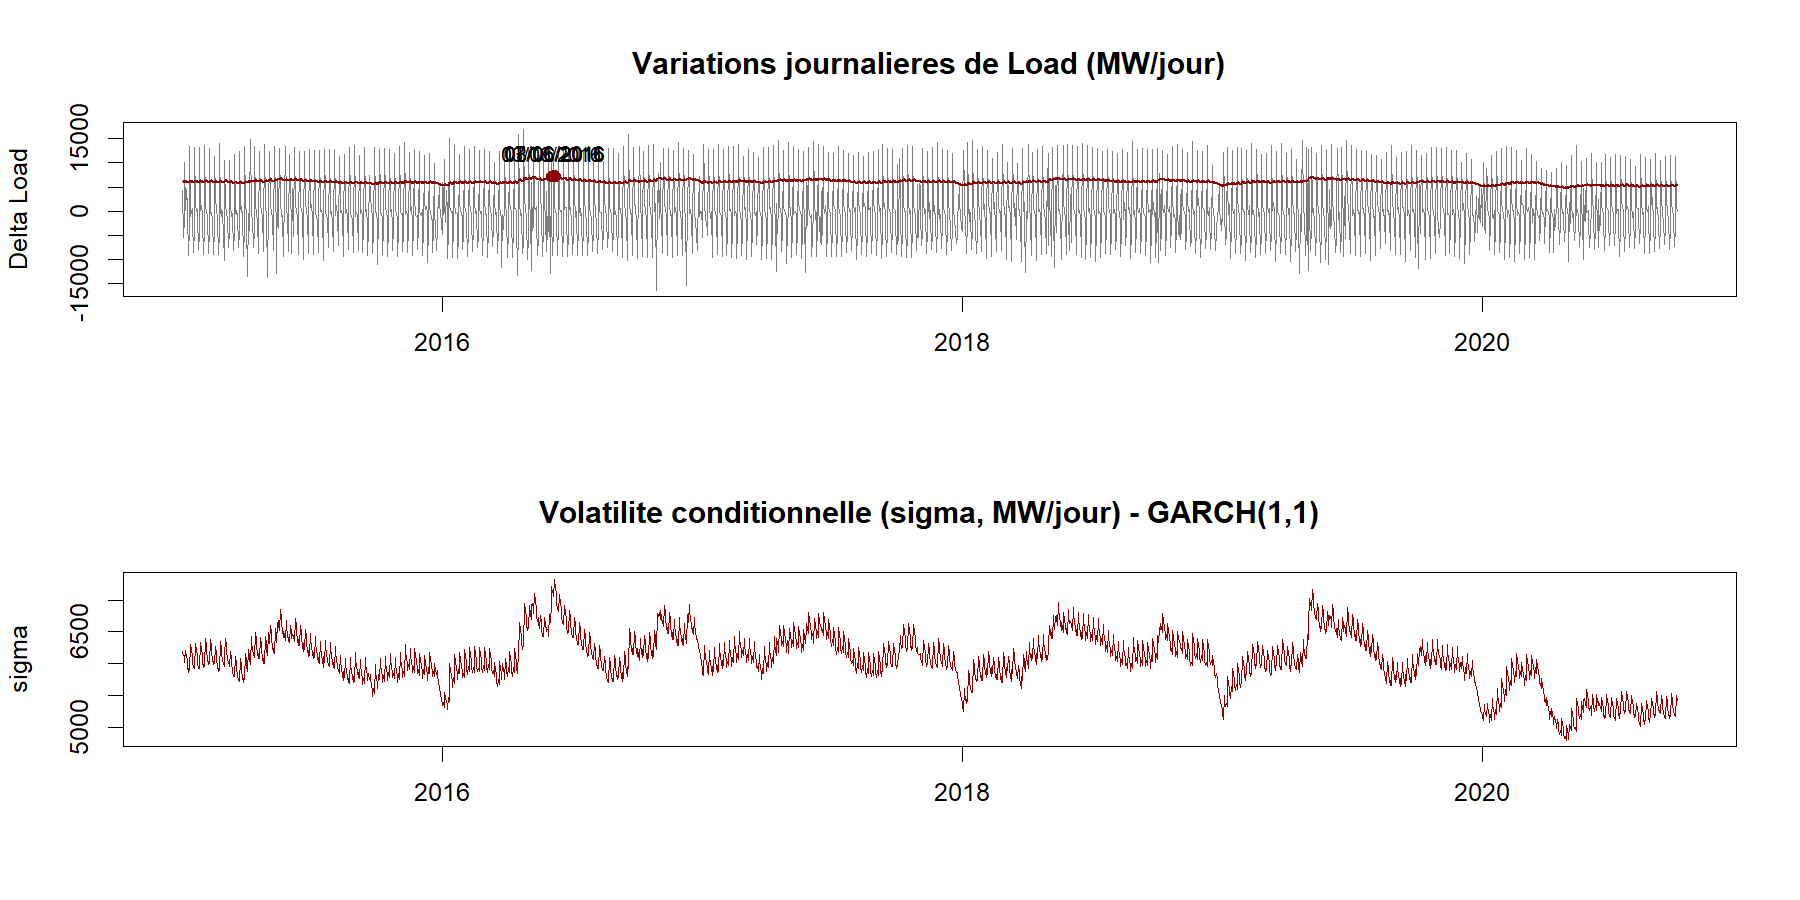
\includegraphics[width=0.9\textwidth]{R_garch_Load.png}
\caption{Volatilité conditionnelle \texttt{Load} (GARCH(1,1), R).}
\label{fig:garch_r_load}
\end{figure}

\begin{figure}[H]
\centering
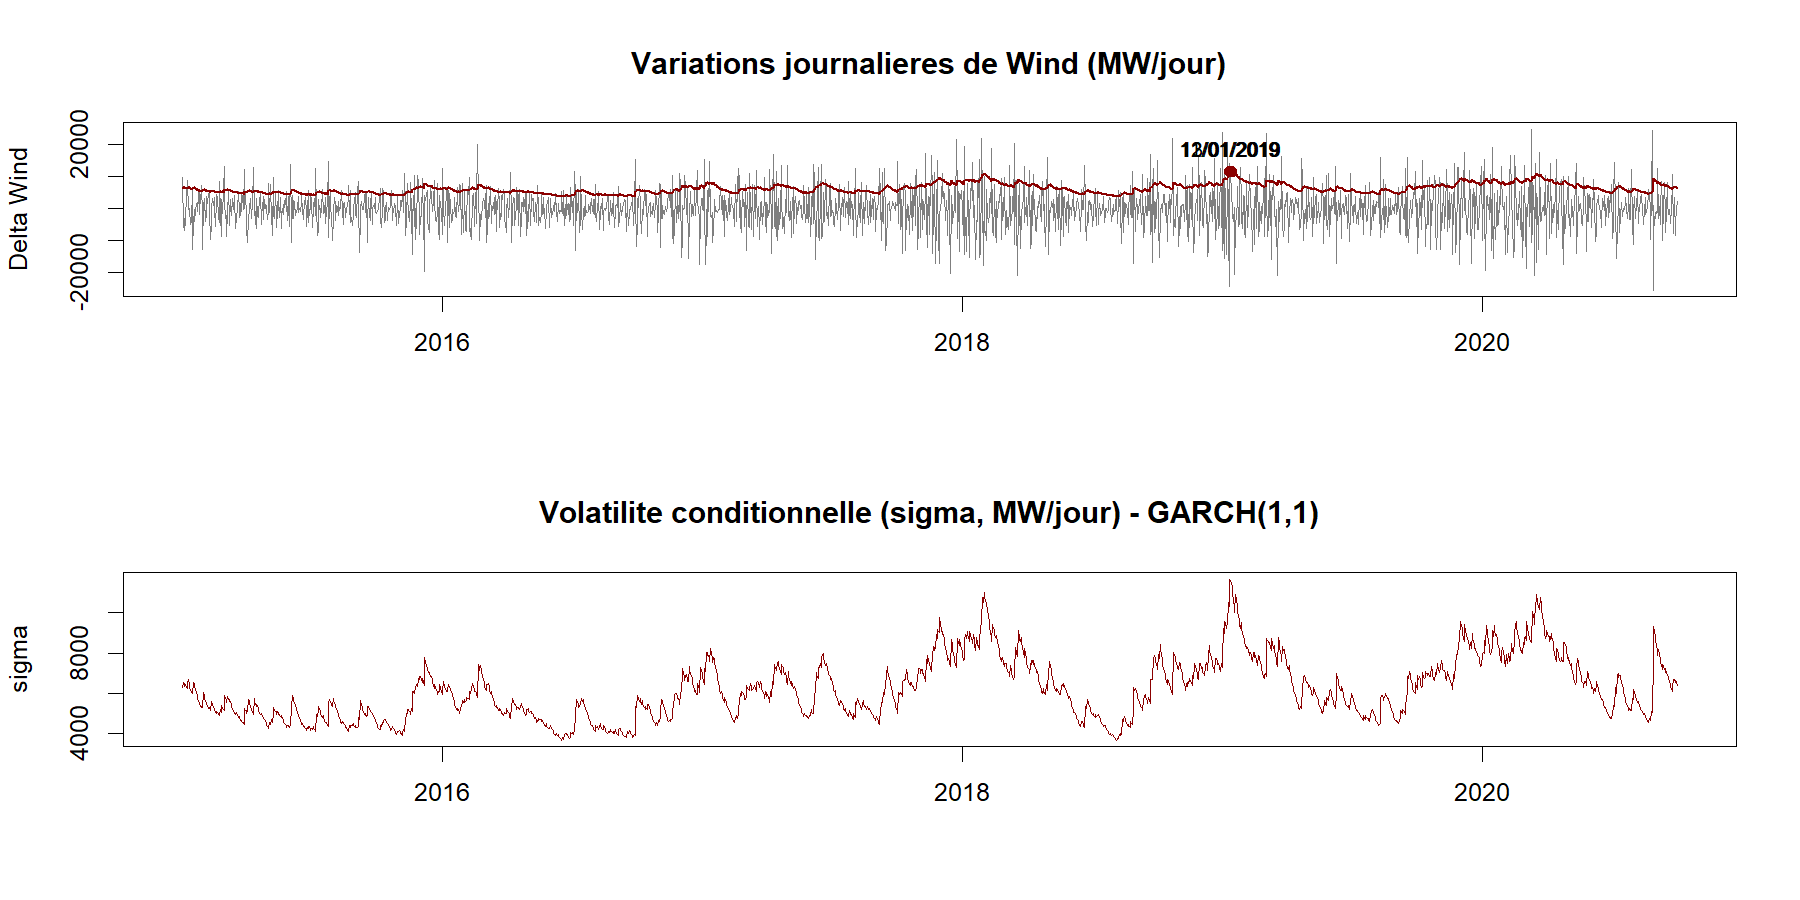
\includegraphics[width=0.9\textwidth]{R_garch_Wind.png}
\caption{Volatilité conditionnelle \texttt{Wind} (GARCH(1,1), R).}
\label{fig:garch_r_wind}
\end{figure}

\begin{figure}[H]
\centering
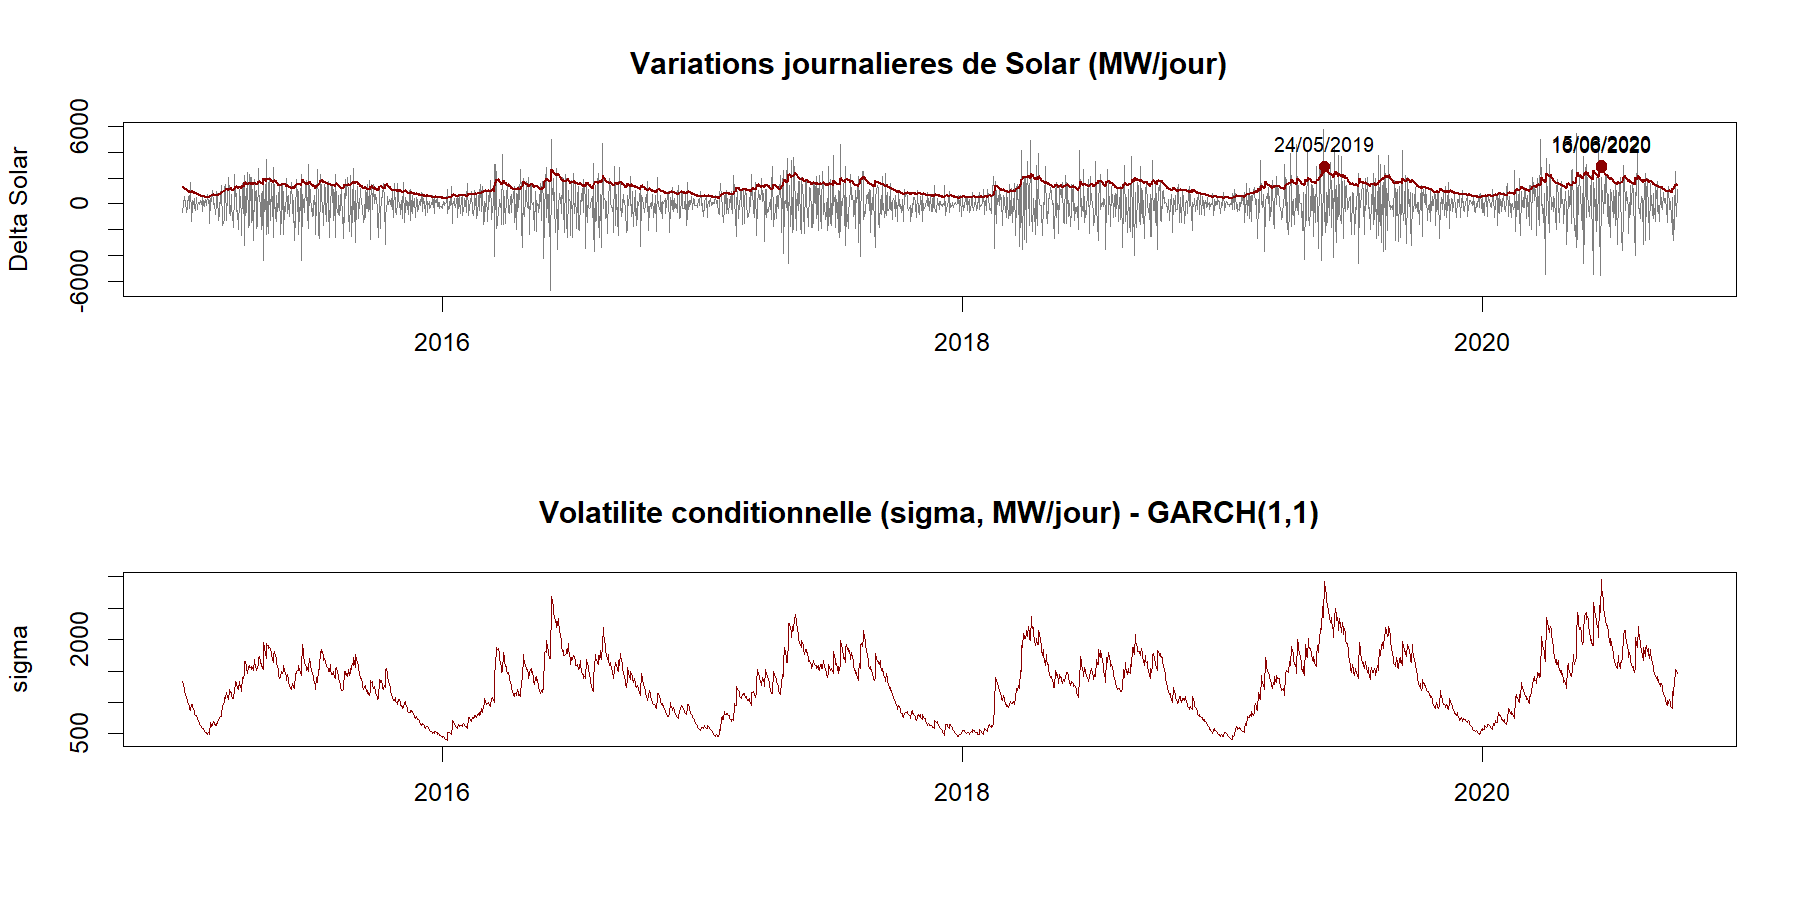
\includegraphics[width=0.9\textwidth]{R_garch_Solar.png}
\caption{Volatilité conditionnelle \texttt{Solar} (GARCH(1,1), R).}
\label{fig:garch_r_solar}
\end{figure}

\begin{figure}[H]
\centering
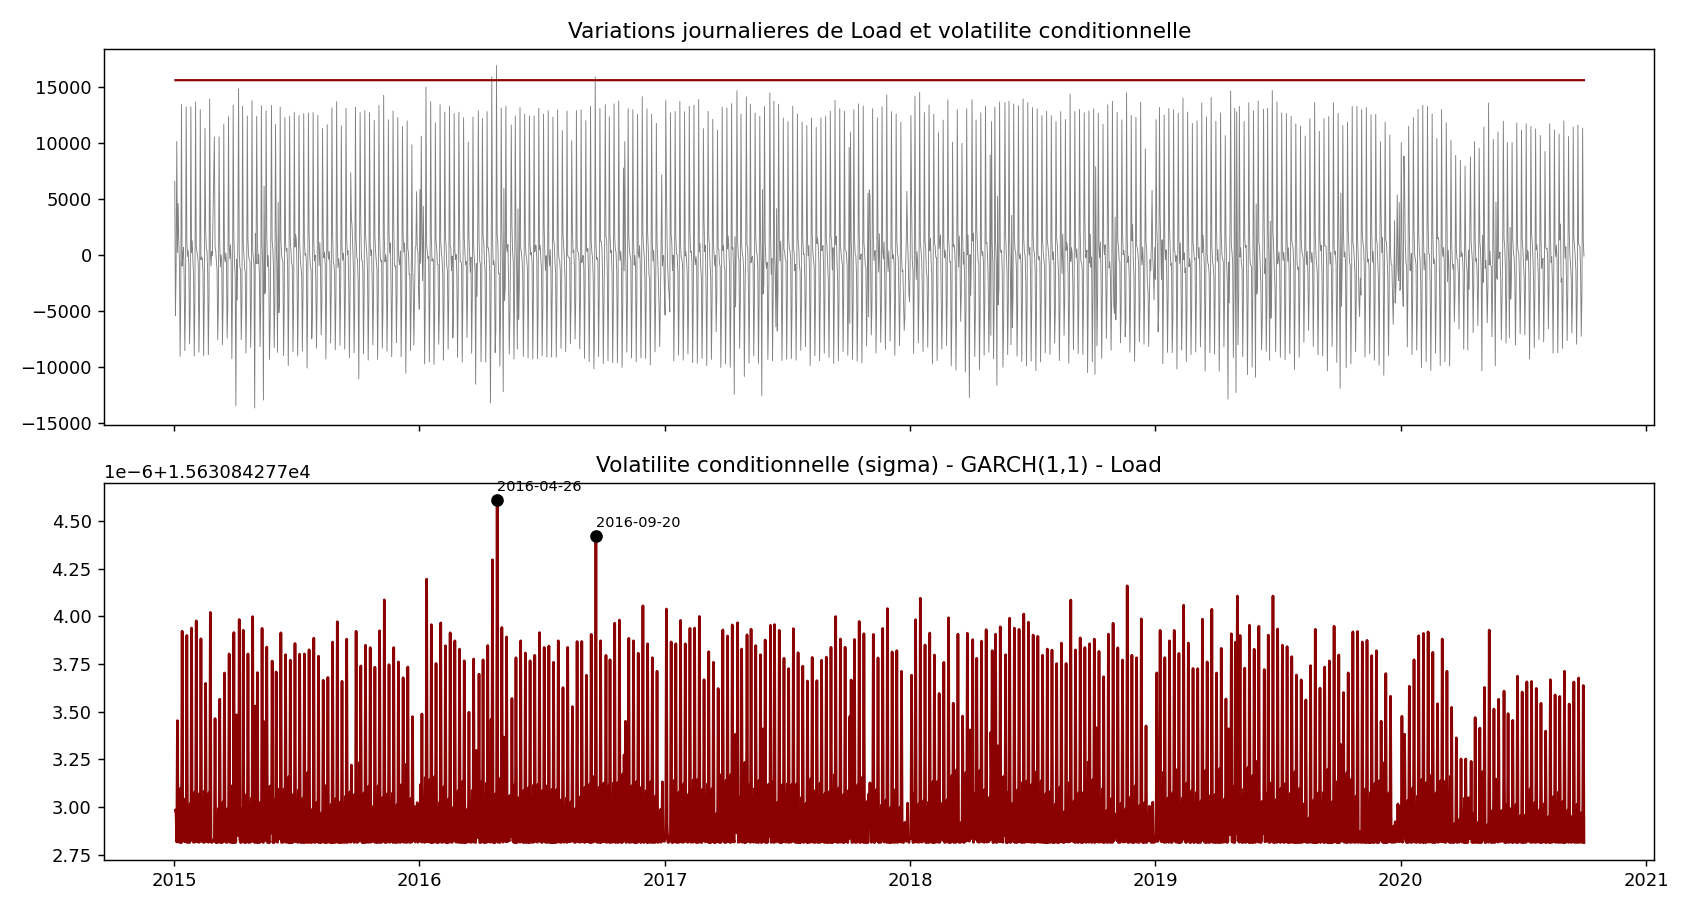
\includegraphics[width=0.9\textwidth]{py_garch_Load.png}
\caption{Volatilité conditionnelle \texttt{Load} (Python).}
\label{fig:garch_py_load}
\end{figure}

\begin{figure}[H]
\centering
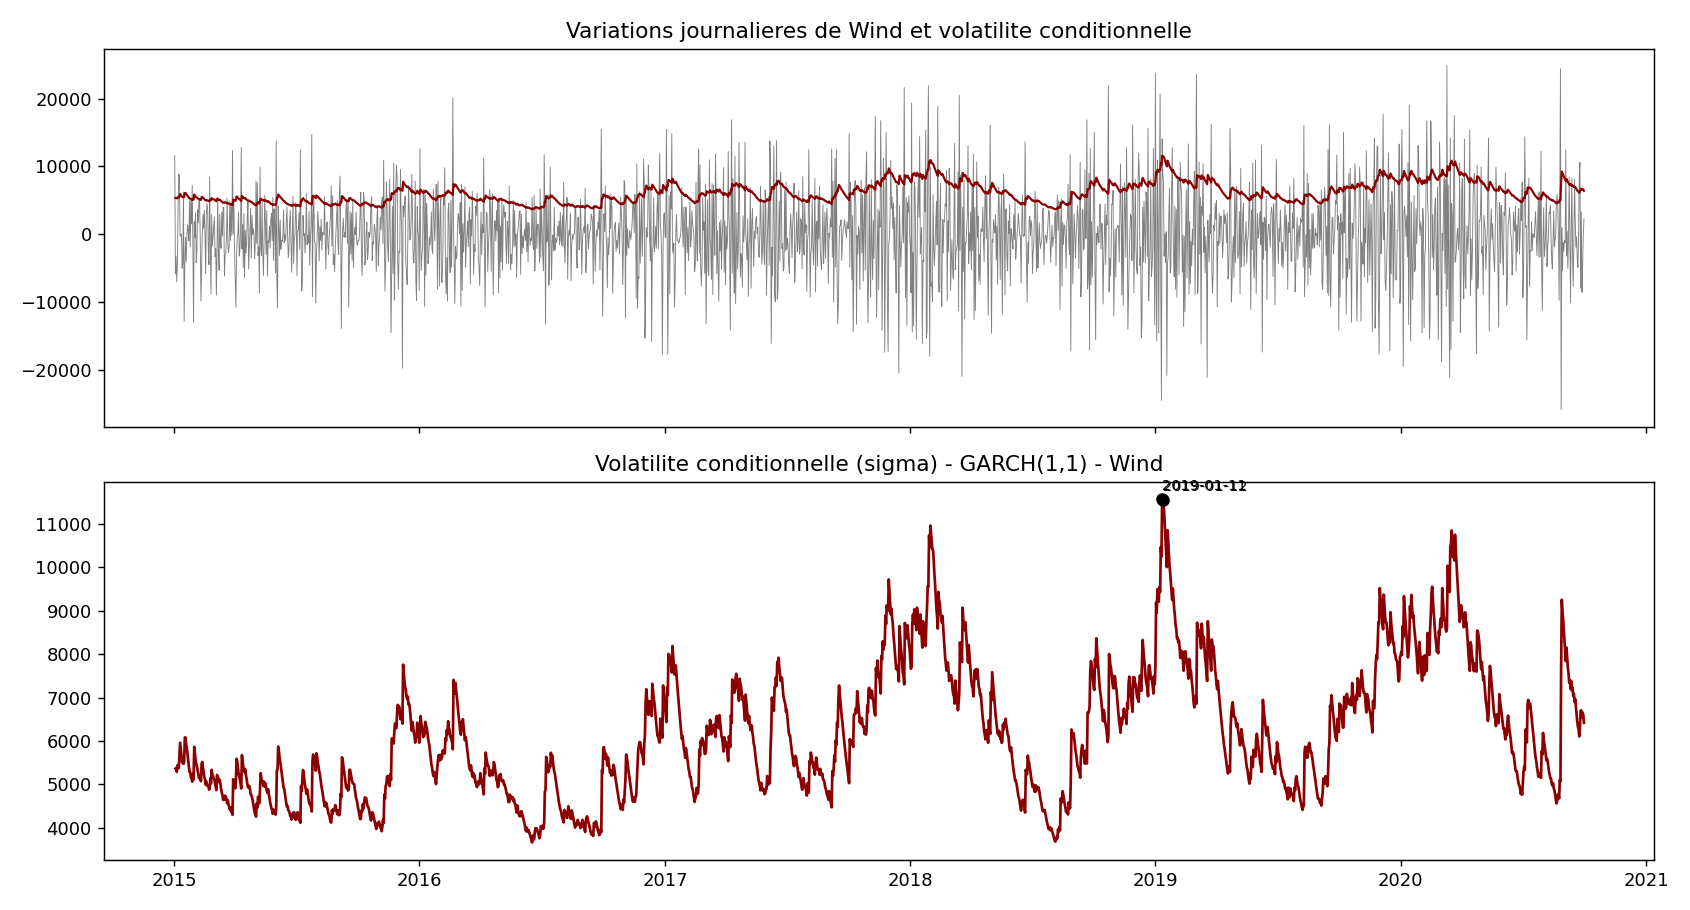
\includegraphics[width=0.9\textwidth]{py_garch_Wind.png}
\caption{Volatilité conditionnelle \texttt{Wind} (Python).}
\label{fig:garch_py_wind}
\end{figure}

\begin{figure}[H]
\centering
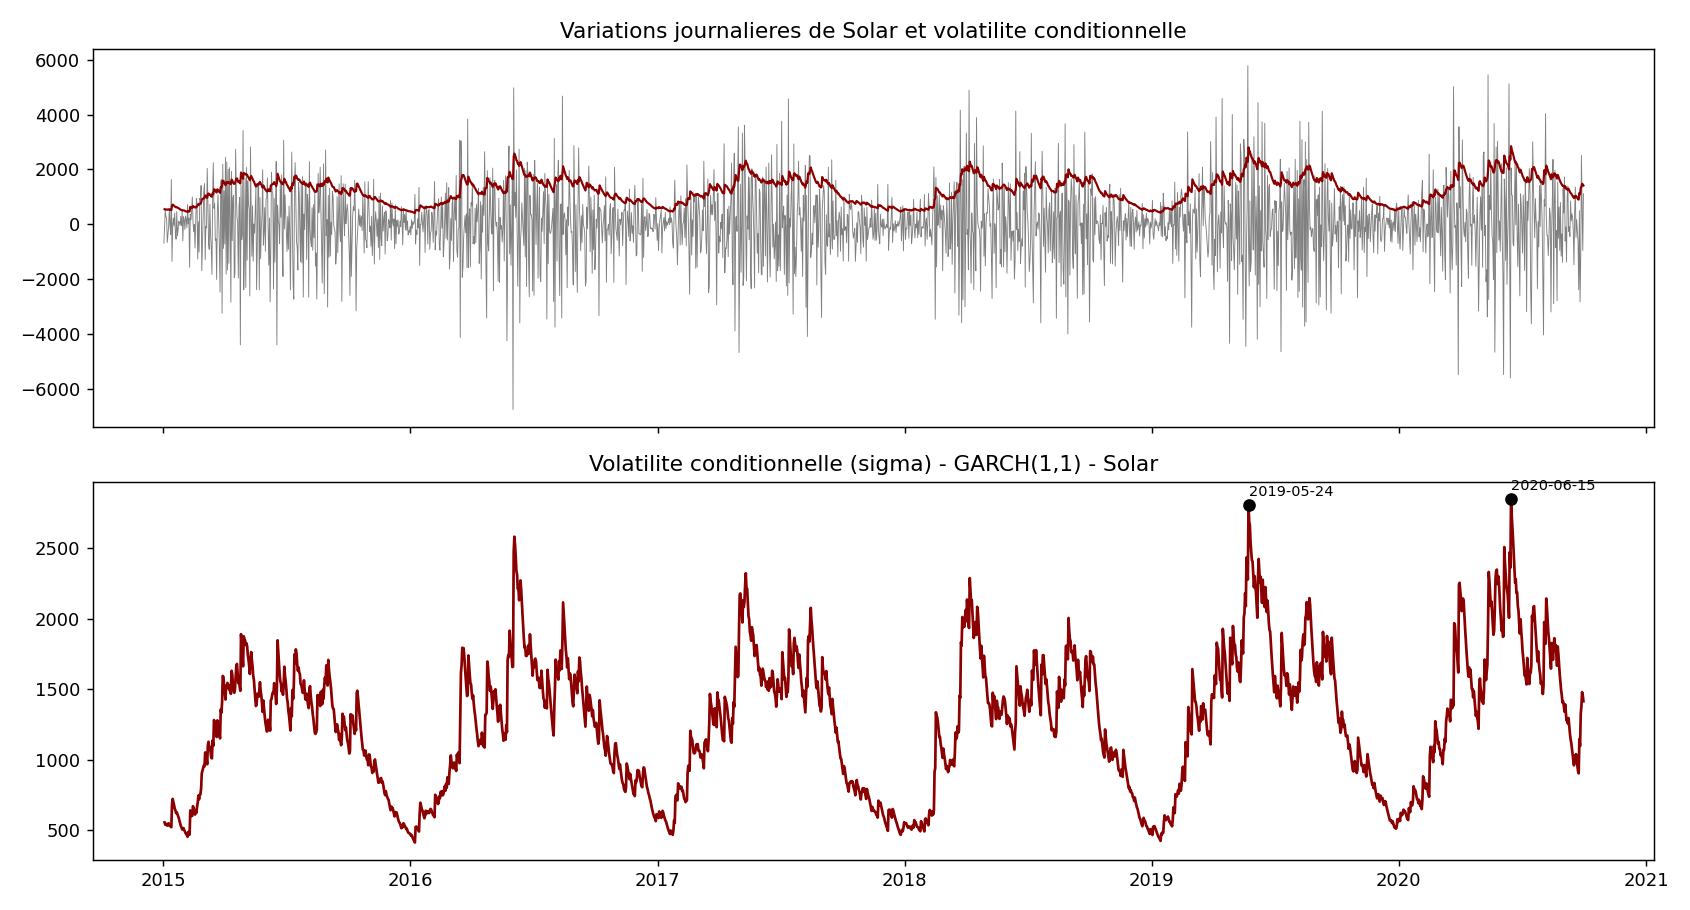
\includegraphics[width=0.9\textwidth]{py_garch_Solar.png}
\caption{Volatilité conditionnelle \texttt{Solar} (Python).}
\label{fig:garch_py_solar}
\end{figure}

\FloatBarrier

\subsection{Modèles profonds : LSTM / GRU}

Deux architectures récurrentes (LSTM et GRU), régularisées par une couche de
\textbf{Dropout} (\(p=0{,}2\)), sont entraînées par série avec une fenêtre
glissante de \(168\)~h et une prévision récursive ; la meilleure architecture
(sur la \texttt{val\_loss}) est conservée. Le tableau~\ref{tab:lstm} présente
les métriques des deux réseaux : la sélection retient le \textbf{LSTM} pour
\texttt{Load} et \texttt{Solar}, le \textbf{GRU} pour \texttt{Wind}. À
\(h=10\), le LSTM atteint une RMSE de \(1\,263{,}0\)~MW sur \texttt{Load}
(\(\text{MAPE}=1{,}57\,\%\)). À \(h=5\,040\), le LSTM reste le plus performant
sur \texttt{Load} (\(7\,592{,}7\)~MW, à comparer aux \(65\,847\)~MW de
SARIMA\_manuel), tandis que le GRU domine sur \texttt{Wind}
(\(8\,567{,}3\)~MW contre \(11\,858{,}4\) pour le LSTM). Sur \texttt{Solar}, le
MAPE devient astronomique (\(\sim 1{,}7\times 10^{14}\,\%\)) : artefact
documenté dû aux valeurs proches de zéro la nuit.

\begin{table}[H]
\centering
\caption{Métriques LSTM/GRU (Python).
Source : \texttt{py\_lstm\_gru\_metrics.csv}.}
\label{tab:lstm}
\small
\begin{tabular}{llrrrr}
\toprule
Variable & Modèle & $h$ & RMSE & MAE & MAPE (\%) \\
\midrule
\texttt{Load}  & LSTM & 10 & 1\,263{,}0 & 967{,}8 & 1{,}57 \\
\texttt{Load}  & LSTM & 24 & 1\,918{,}7 & 1\,555{,}9 & 2{,}44 \\
\texttt{Load}  & LSTM & 5040 & 7\,592{,}7 & 6\,137{,}2 & 13{,}00 \\
\texttt{Load}  & GRU & 10 & 2\,708{,}3 & 2\,259{,}0 & 3{,}60 \\
\texttt{Load}  & GRU & 24 & 8\,406{,}2 & 6\,593{,}0 & 9{,}95 \\
\texttt{Load}  & GRU & 5040 & 9\,033{,}5 & 7\,809{,}0 & 15{,}83 \\
\texttt{Wind}  & LSTM & 10 & 3\,120{,}0 & 2\,819{,}3 & 45{,}38 \\
\texttt{Wind}  & LSTM & 24 & 7\,870{,}1 & 6\,203{,}7 & 42{,}78 \\
\texttt{Wind}  & LSTM & 5040 & 11\,858{,}4 & 10\,584{,}9 & 296{,}93 \\
\texttt{Wind}  & GRU & 10 & 2\,060{,}4 & 1\,847{,}2 & 29{,}89 \\
\texttt{Wind}  & GRU & 24 & 9\,277{,}6 & 6\,759{,}1 & 38{,}99 \\
\texttt{Wind}  & GRU & 5040 & 8\,567{,}3 & 6\,993{,}9 & 172{,}26 \\
\texttt{Solar} & LSTM & 10 & 573{,}8 & 420{,}1 & $5{,}9\text{e}12$ \\
\texttt{Solar} & LSTM & 24 & 579{,}0 & 447{,}7 & $6{,}1\text{e}12$ \\
\texttt{Solar} & LSTM & 5040 & 11\,368{,}4 & 8\,398{,}9 & $1{,}7\text{e}14$ \\
\texttt{Solar} & GRU & 10 & 3\,334{,}2 & 2\,480{,}1 & $6{,}2\text{e}13$ \\
\texttt{Solar} & GRU & 24 & 4\,092{,}7 & 3\,171{,}4 & $8{,}4\text{e}13$ \\
\texttt{Solar} & GRU & 5040 & 10\,534{,}3 & 7\,430{,}5 & $8{,}8\text{e}13$ \\
\bottomrule
\end{tabular}
\end{table}

\paragraph{Validation croisée temporelle (TSCV).}
Une validation croisée à fenêtre expansive (\(k=3\) plis) confirme la
stabilité des réseaux : la RMSE de validation décroît puis se stabilise à
mesure que le train s'allonge (\texttt{Load}\,: \(2\,178\to1\,907\)~MW pour le
LSTM ; \texttt{Wind}\,: \(957\to876\)~MW pour le GRU ; \texttt{Solar}\,:
\(1\,422\to1\,146\)~MW pour le LSTM). Source :
\texttt{py\_lstm\_gru\_cv.csv}.

Les figures~\ref{fig:lstm_forecast_load}--\ref{fig:lstm_forecast_solar}
comparent prévisions et valeurs réelles, et les figures de \emph{loss}
(\ref{fig:lstm_loss_load}--\ref{fig:lstm_loss_solar}) illustrent la
convergence de l'apprentissage (train/validation).

\begin{figure}[H]
\centering
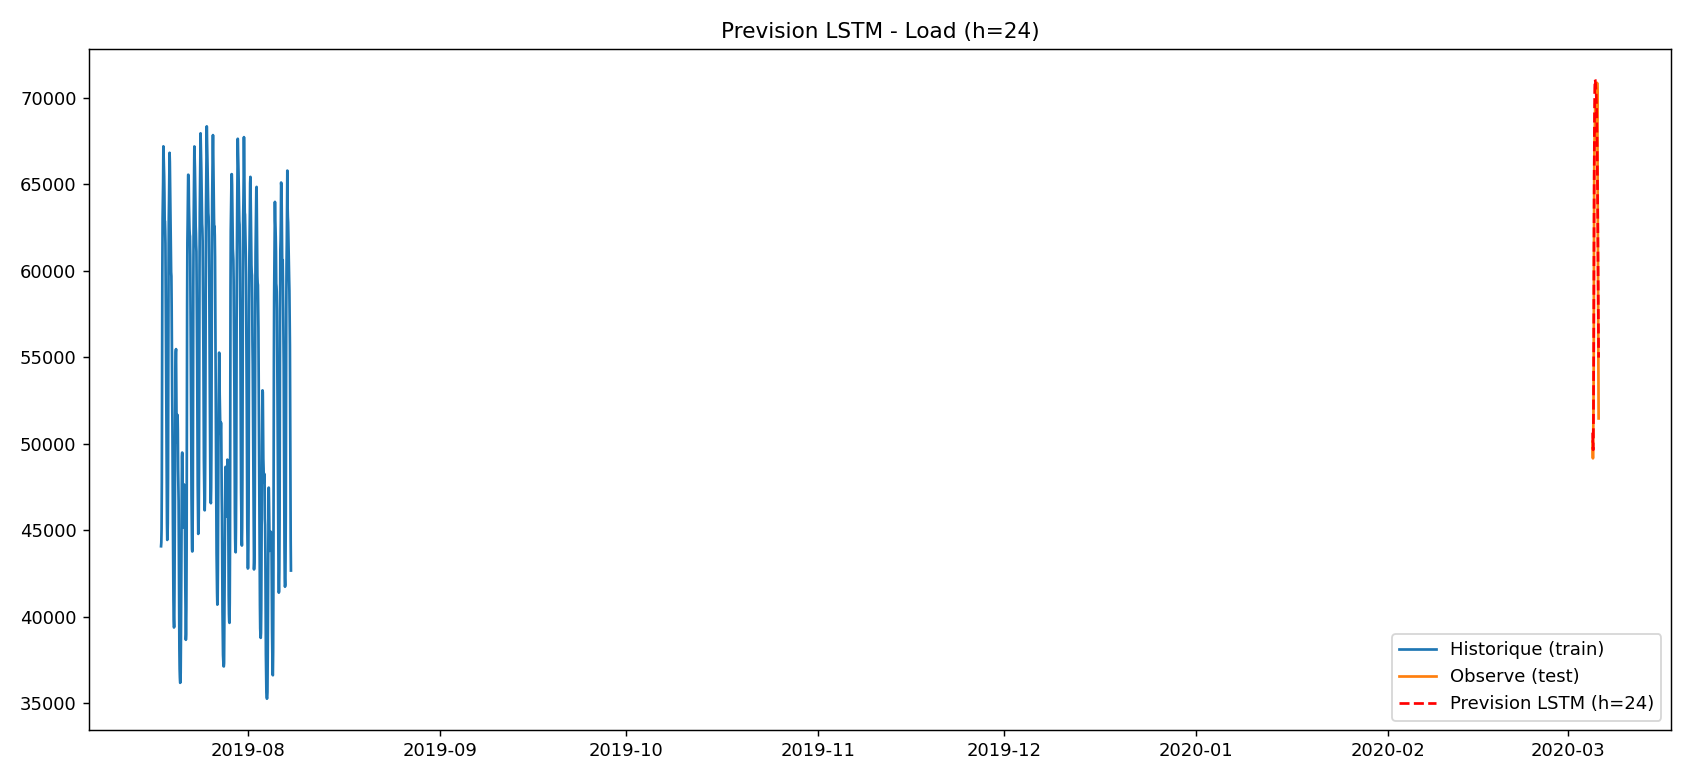
\includegraphics[width=0.9\textwidth]{py_lstm_gru_forecast_Load.png}
\caption{Prévisions LSTM/GRU -- \texttt{Load}.}
\label{fig:lstm_forecast_load}
\end{figure}

\begin{figure}[H]
\centering
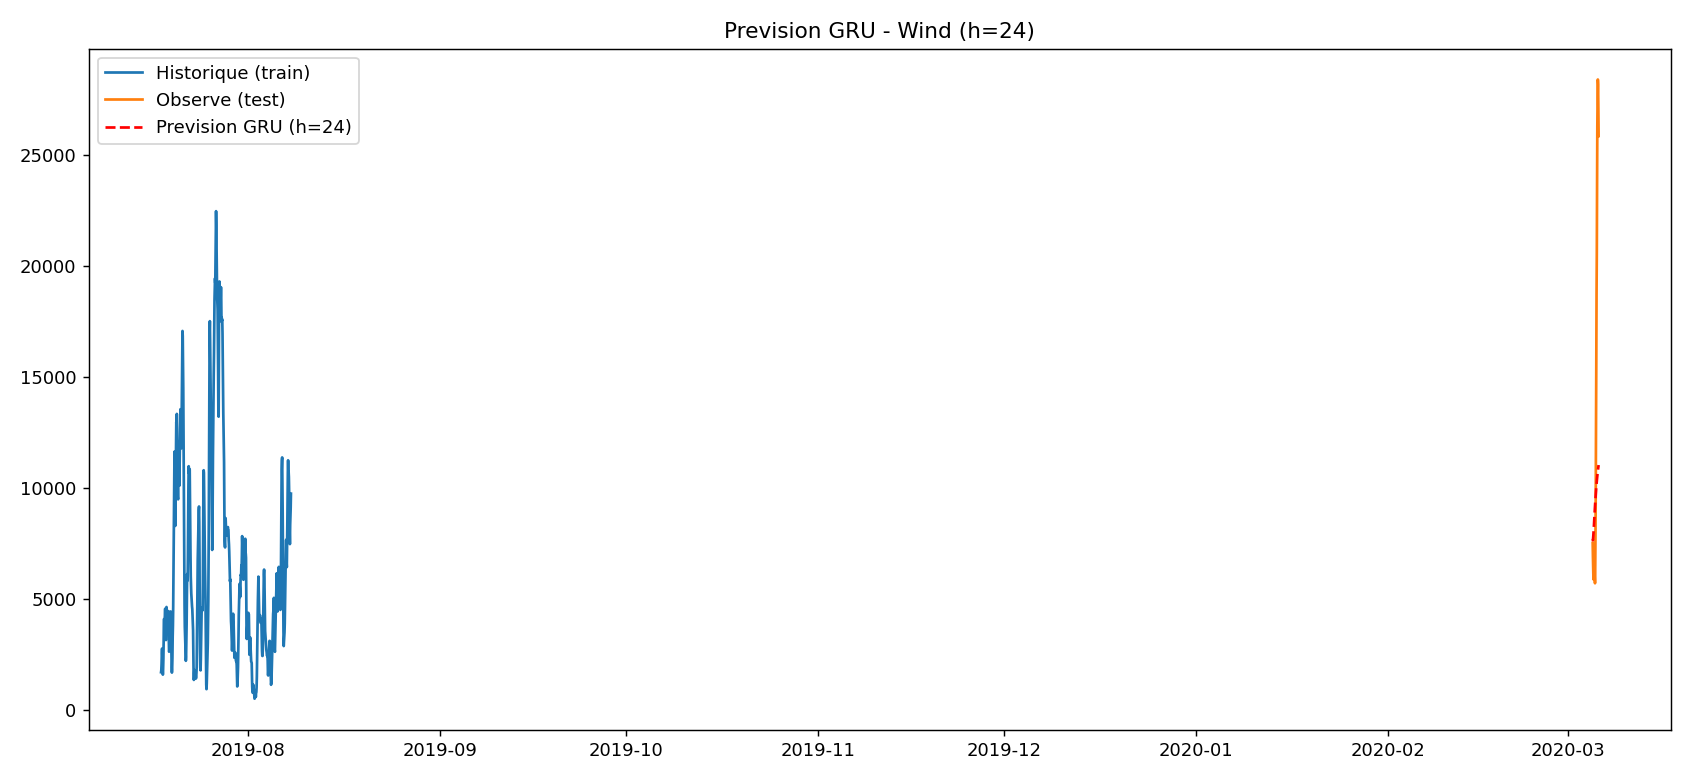
\includegraphics[width=0.9\textwidth]{py_lstm_gru_forecast_Wind.png}
\caption{Prévisions LSTM/GRU -- \texttt{Wind}.}
\label{fig:lstm_forecast_wind}
\end{figure}

\begin{figure}[H]
\centering
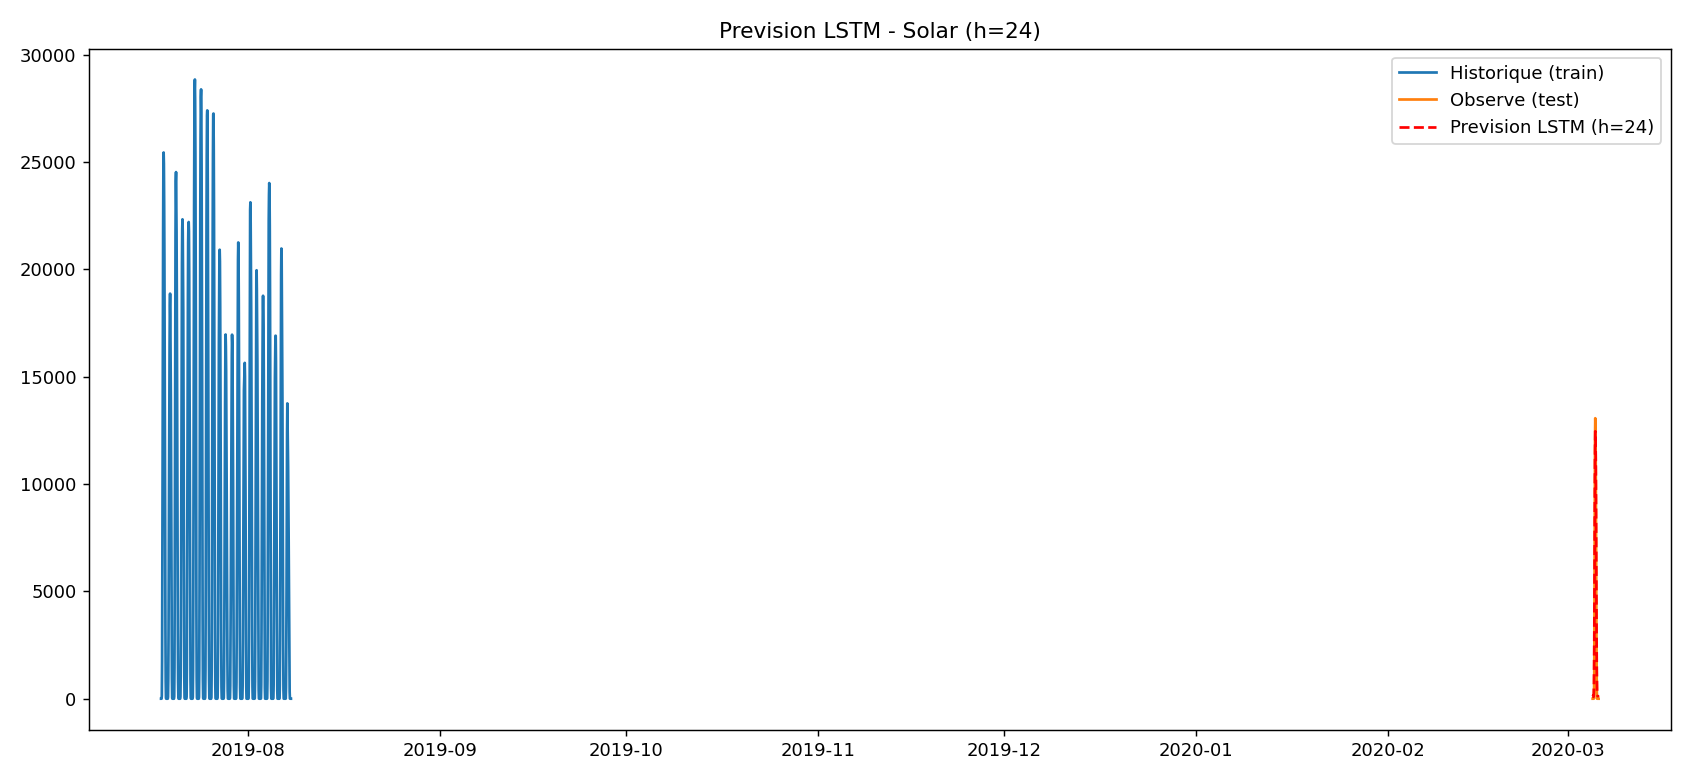
\includegraphics[width=0.9\textwidth]{py_lstm_gru_forecast_Solar.png}
\caption{Prévisions LSTM/GRU -- \texttt{Solar}.}
\label{fig:lstm_forecast_solar}
\end{figure}

\begin{figure}[H]
\centering
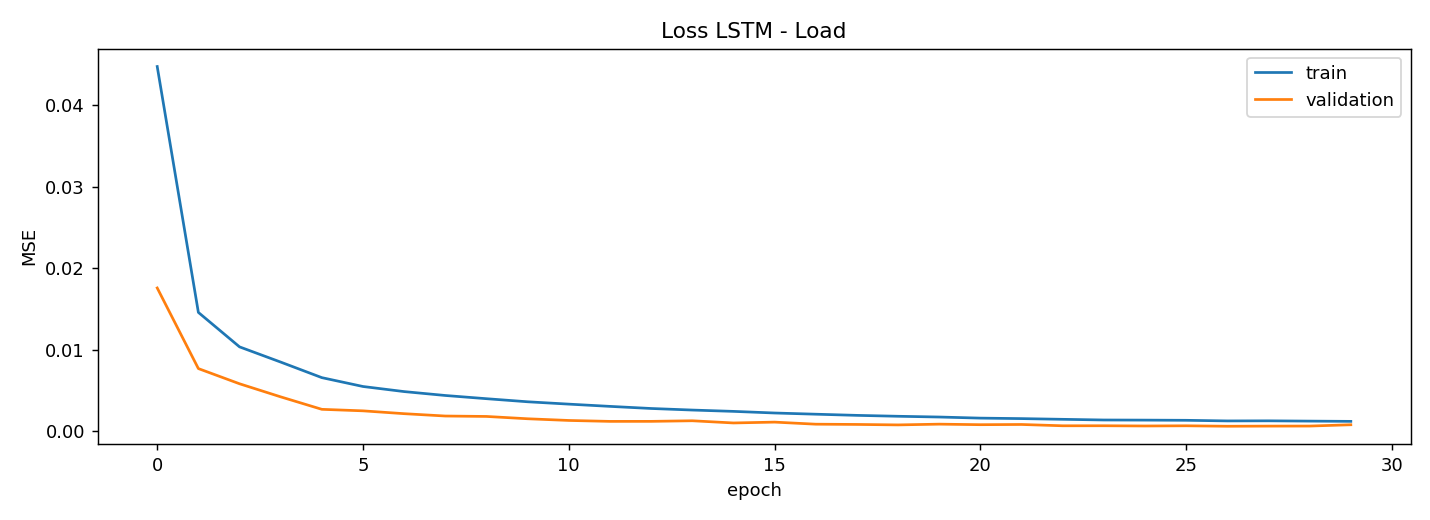
\includegraphics[width=0.75\textwidth]{py_lstm_gru_loss_Load.png}
\caption{Courbes de \emph{loss} -- \texttt{Load}.}
\label{fig:lstm_loss_load}
\end{figure}

\begin{figure}[H]
\centering
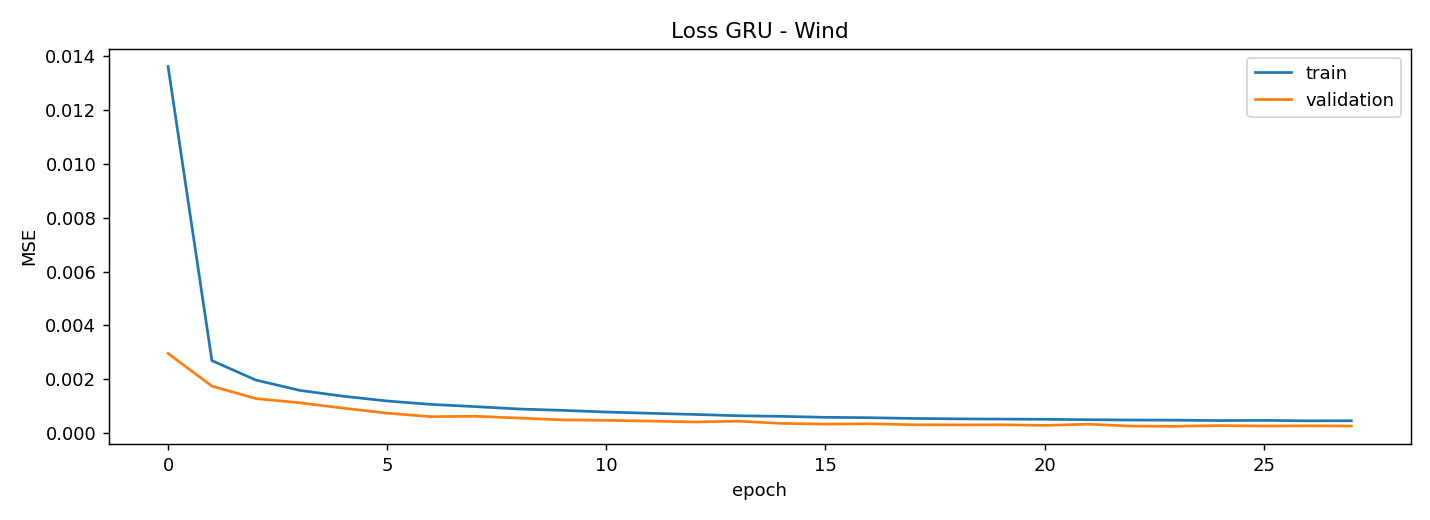
\includegraphics[width=0.75\textwidth]{py_lstm_gru_loss_Wind.png}
\caption{Courbes de \emph{loss} -- \texttt{Wind}.}
\label{fig:lstm_loss_wind}
\end{figure}

\begin{figure}[H]
\centering
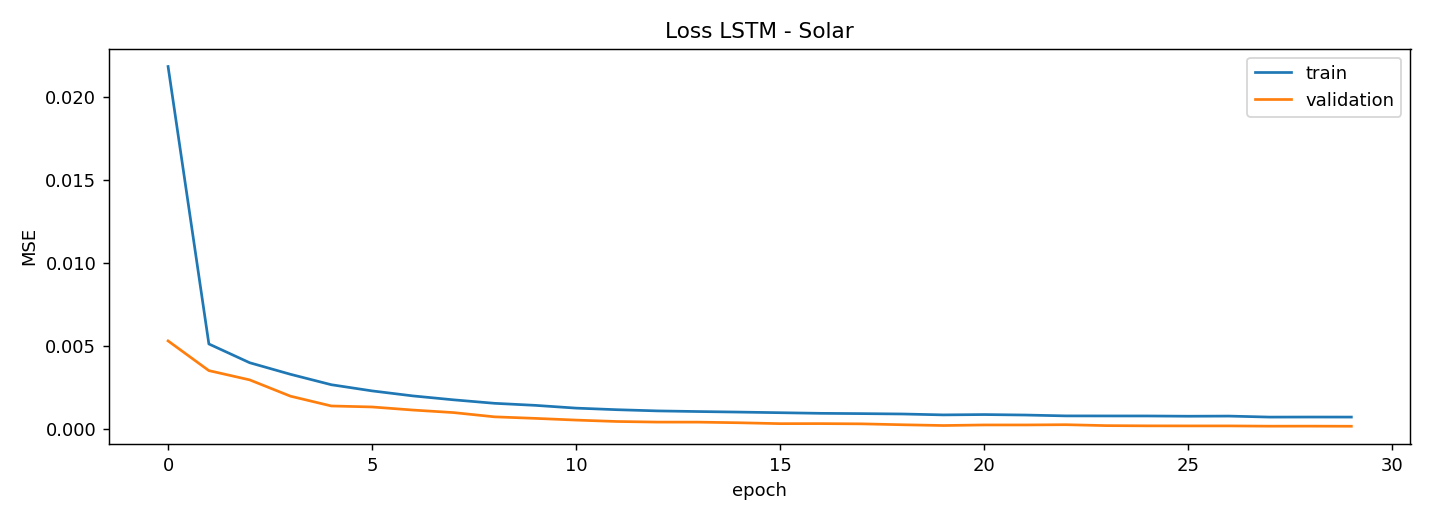
\includegraphics[width=0.75\textwidth]{py_lstm_gru_loss_Solar.png}
\caption{Courbes de \emph{loss} -- \texttt{Solar}.}
\label{fig:lstm_loss_solar}
\end{figure}

\FloatBarrier
